\documentclass[11pt,a4paper]{article}

\usepackage[margin=2.4cm]{geometry}
\usepackage{graphicx}
\usepackage{amsmath,amssymb}
\usepackage{booktabs}
\usepackage{array}
\usepackage{xcolor}
\usepackage{tikz}
\usepackage{float}
\usetikzlibrary{shapes.geometric,arrows.meta,positioning,fit,calc}
\usepackage[most]{tcolorbox}
\usepackage{caption}
\usepackage{subcaption}
\usepackage{hyperref}
\usepackage{enumitem}
\usepackage{fancyhdr}

\hypersetup{colorlinks=true, linkcolor=blue!60!black, urlcolor=blue!60!black,
            citecolor=blue!60!black}
\pagestyle{fancy}
\fancyhf{}
\fancyhead[L]{\small Swarm Cooperative Transport --- Simulation Report}
\fancyhead[R]{\small\thepage}

\newtcolorbox{keybox}[1]{colback=blue!4,colframe=blue!45!black,
  fonttitle=\bfseries,title={#1},boxrule=0.6pt,arc=2pt}

\newcommand{\code}[1]{\texttt{#1}}
\newcommand{\param}[2]{\code{#1}~\texttt{=}~#2}

\title{\textbf{Dynamic-Obstacle Swarm Cooperative Transport}\\[4pt]
\large The kinematic model, its algorithms and parameters, and how to read\\every graph\\[6pt]
\normalsize Simulation report for \code{Simulation8_dynamic.m}}
\author{Swarm Transport Project}
\date{October 2026}

\begin{document}
\maketitle
\thispagestyle{empty}

\begin{abstract}
\noindent
Four differential-drive robots start scattered in a warehouse, assemble into a
rigid $2\times2$ formation that physically carries a payload, and transport it
through a corridor network that contains both static obstacles (walls, shelf
racks, pillars, pallets) and \emph{moving} obstacles (kinematic forklifts and
a drum following a shared motion contract). The whole stack is a kinematic
model --- unicycle geometry, potential-field goal seeking, polar histogram
obstacle avoidance, rigid-frame transport --- evaluated at 10~Hz against an
exact signed-distance representation of the world. Eight steering laws are
compared on scans from one shared, seeded sensor front end: an APF reflex,
deterministic VFH+ with and without a mover-prediction horizon,
Follow-the-Gap, a Dynamic-Window planner, a receding-horizon MPC, and the
proposal, \textbf{P-VFH},
which replaces the deterministic histogram occupancy with the posterior
expectation of the danger kernel under the sensor's range uncertainty. That
kernel reduces to the deterministic one as the noise vanishes and widens the
reaction envelope as it grows (both proved); it is combined with a recursive
range filter whose gain is set by the sensor noise model, and an ablation
law separates the two. This report documents the
model, the algorithms and every parameter, teaches the concepts, and
presents a fourteen-experiment Monte Carlo evaluation (E1--E14) over three
designed and ten randomly generated environments whose tables and figures are generated from a single results
file. An audit in October 2026 (\S\ref{sec:audit}) found and fixed defects
in the reference code that had produced the collision counts reported in
earlier drafts; results obtained before that audit are superseded. On the corrected code (2,730 runs) the range filter removes most of
the histogram's sensitivity to range noise in corridor and maze
environments, while the expected kernel is not shown to add anything in a
matched ablation; an MPC baseline is faster at normal traffic in the
warehouse and better in an open plaza, while the histogram laws match it
on random layouts and degrade more gracefully as traffic gets faster or
denser (\S\ref{sec:findings}). An October 2026 independent replication
(\S\ref{sec:replication}) then brought the Python and ROS 2 stacks to
agree with the MATLAB grid in 220 of 221 cells, and a MuJoCo run showed
where the kinematic model stops being predictive. All
validation here is in simulation (\S\ref{sec:simvalidation} states what
that does and does not establish).
\end{abstract}

\tableofcontents
\newpage

\section{The model}
\label{sec:model-kinematics}

\subsection{What kind of model this is}

The simulation is a \textbf{kinematic} model. It contains no forces, masses or
inertia: every motion constraint is imposed directly on \emph{rates}. A robot
is a point with a heading; a formation is a rigid geometric body; an obstacle
is a region of $\mathbb{R}^2$ with an exact signed distance.

\begin{keybox}{State and update (the unicycle model)}
For every agent (each robot in Phase~1, the formation frame in Phase~2), with
position $\mathbf{p} = (x, y)$ and heading $\theta$, evaluated at
$\Delta t = 0.1$~s:
\begin{align}
\mathbf{p}_{k+1} &= \mathbf{p}_k + v_k \, \begin{bmatrix}\cos\theta_k \\ \sin\theta_k\end{bmatrix} \Delta t, \\[4pt]
\theta_{k+1} &= \theta_k + \operatorname{clip}\bigl(\operatorname{wrap}(\theta_{\mathrm{des}} - \theta_k),\; \pm\omega_{\max}\bigr),
\end{align}
with the desired heading first low-pass smoothed:
\[
\theta_{\mathrm{des}} = \theta_k + \alpha\,\operatorname{wrap}(\theta_{\mathrm{raw}} - \theta_k),
\qquad \alpha = 0.35 .
\]
\end{keybox}

The low-pass on heading is not cosmetic. In Phase~2 the heading \emph{is} the
payload's orientation; $\alpha = 0.35$ converts the raw obstacle-avoidance
command (which can zig-zag at the controller rate) into a smooth yaw profile,
i.e.\ the load is never yanked. The cost is a slightly lazier obstacle
response, which the prediction layer (Section~\ref{sec:dynamic}) pays for.

Speeds are \emph{prescribed}, not controlled dynamics:
$v = V = 0.6$~m/s in transport, $v = V_{\mathrm{form}} = 0.5$~m/s in forming,
both modulated by the proximity logic of Section~\ref{sec:algorithms}.
Because velocity is a decision variable rather than a state, the model
integrates exactly --- there is no numerical stiffness, and a MATLAB run and a
ROS~2 run differ only through tracking error, never through integration error.

\subsection{The world representation: one signed distance to rule them all}

The Gazebo SDF world is parsed into boxes (centre, yaw, half-extents) and
circles (centre, radius) at the robot's height band
$z \in [0.03, 0.35]$~m (so the 2~cm goal pad is not an obstacle but the 60~cm
pallets are). Every geometric question is then answered by a single primitive,
the \textbf{exact signed distance} $d(\mathbf{p})$ from \code{world\_dist.m}:

\[
d(\mathbf{p}) =
\begin{cases}
>0 & \text{free space (distance to the nearest surface)}\\
=0 & \text{on a surface}\\
<0 & \text{inside an obstacle}
\end{cases}
\]

\begin{center}
\begin{tabular}{@{}ll@{}}
\toprule
\textbf{Question} & \textbf{Answer in terms of $d$}\\
\midrule
Is this pose in collision? & $d \le 0$\\
Is this pose safe for a robot of radius $r$? & $d > r$\\
Clearance metric of the run & $d$ itself, minimised over the body\\
Raycast for the LiDAR & slab method / quadratic against the same primitives\\
Feasibility of a corridor & flood fill over a thresholded grid of $d$\\
\bottomrule
\end{tabular}
\end{center}

Because the primitive is exact and shared, a ``collision'' in the simulation
means the same thing a physics engine's contact report would mean --- which is
what makes the MATLAB and ROS~2 runs comparable at all.

\subsection{Two-phase mission}

\begin{enumerate}[leftmargin=1.6em]
\item \textbf{Phase 1 --- forming up.} Robots start scattered on a ring of
radius $2.2$~m around the start point. Each runs its own controller to reach
an assigned slot. Success: every robot within $0.3$~m of its slot.
\item \textbf{Phase 2 --- rigid transport.} The formation becomes one rigid
body: a virtual leader (the frame centre) runs a single controller; the four
robots are \emph{slaves of the frame}, $\mathbf{p}_i = \mathbf{c} + R(\theta)\,
\mathbf{o}_i$. The payload is the block spanned by the formation.
\end{enumerate}

The two phases use the same two algorithms (APF, p-VFH) but \emph{different
compositions} of them --- cascaded in Phase~1, weighted-sum in Phase~2 --- as
summarised in Table~\ref{tab:arch}.

\section{The algorithms}
\label{sec:algorithms}

Three algorithm families carry the whole behaviour: Artificial Potential
Fields (goal seeking and inter-robot spacing), the VFH family (obstacle
avoidance --- deterministic, predictive, and the probabilistic P-VFH proposal
of Section~\ref{sec:pvfh}), and the rigid-transport frame logic that ties the
four robots into one body. They compose into the steering-law variants
compared in Section~\ref{sec:fourvariants}, alongside two external
baselines (Follow-the-Gap, a Dynamic-Window planner and a
receding-horizon MPC, \S\ref{sec:baselines}).

\subsection{Artificial Potential Fields (APF)}

\code{apf\_force.m} computes an unnormalised force as the sum of a conic
attraction and a linear inter-robot repulsion:
%
\begin{align}
\mathbf{F}_{\mathrm{att}} &= w_{\mathrm{att}}\,
\frac{\mathbf{g} - \mathbf{p}}{\lVert \mathbf{g} - \mathbf{p} \rvert}, \\[4pt]
\mathbf{F}_{\mathrm{rep}} &= w_{\mathrm{rep}} \sum_{j \,:\, d_{ij} < d_0}
(d_0 - d_{ij})\, \frac{\mathbf{p} - \mathbf{p}_j}{d_{ij}}, \\[4pt]
\mathbf{F} &= \mathbf{F}_{\mathrm{att}} + \mathbf{F}_{\mathrm{rep}} .
\end{align}
%
Design choices that matter:

\begin{itemize}[leftmargin=1.6em]
\item \textbf{Conic (constant-magnitude) attraction}, not a quadratic well. A
quadratic field makes the robot crawl to a stop far from the goal; here the
approach slowdown is handled explicitly by the caller
($v \propto \min(1, e/r_{\mathrm{slow}})$), so the field itself stays sharp.
\item \textbf{Linear-in-gap repulsion}, exactly zero at $d = d_0$: no force
discontinuity at the boundary of the influence region, hence no chatter when
a neighbour sits at the edge of range.
\item \textbf{Obstacle avoidance is deliberately absent.} APF repulsion from
two nearby obstacle faces can cancel, leaving zero usable gradient --- the
classical local-minimum trap. All obstacle work is done by VFH.
\end{itemize}

\subsection{p-VFH: polar histogram obstacle avoidance}

\code{pvfh\_scan.m} consumes a \emph{LaserScan} (exactly what a ROS~2 node
reads off \code{/scan}), not a point cloud. Pipeline:

\begin{enumerate}[leftmargin=1.9em]
\item \textbf{Sense.} Analytic raycast, $n_{\mathrm{beams}} = 288$ over
$(-\pi, \pi]$ (open interval --- no duplicated beam at the seam), range
$d_{\mathrm{sense}} = 4.0 + \text{margin}$.
\item \textbf{Polar obstacle density.} $S = 72$ sectors; each sector takes the
\emph{nearest} hit along its bearing and accumulates
$h(s) = \exp(-d^2 / 2\sigma^2)$, with
$\sigma$ \emph{derived} from the required clearance:
$\sigma = (r_{\mathrm{eff}} + g_{\mathrm{react}})\,/\,\sqrt{2\ln(1/\tau)}$.
A fixed $\sigma$ silently hard-codes a fixed reaction distance; deriving it
keeps the reaction margin at $g_{\mathrm{react}} = 1.0$~m beyond the body
whatever the body size.
\item \textbf{VFH+ enlargement.} A hit at range $d$ blocks every bearing
within $\gamma = \arcsin(r_{\mathrm{eff}}/d)$ of it --- a body of effective
radius $r_{\mathrm{eff}}$ steered down any of those bearings would still clip
the obstacle. $r_{\mathrm{eff}}$ is the formation circumradius plus the robot
radius, i.e.\ the histogram is built \emph{for the whole payload}, not the
centre point.
\item \textbf{Circular smoothing.} Window 5 over the polar histogram with
wrap-around at $\pm\pi$ (smoothing it as a line segment leaves a seam
directly behind the robot --- a real bug that produced unexplained turns).
\item \textbf{Valley selection.} Candidate sectors with $h < \tau = 0.3$,
restricted to $\pm 45^\circ$ of the goal bearing; cost
$\lvert \operatorname{wrap}(s - \theta_{\mathrm{goal}})\rvert
+ 0.6\,\lvert \operatorname{wrap}(s - \theta_{\mathrm{prev}})\rvert$ (goal
alignment + heading hysteresis).
\item \textbf{Close-range reflex.} A repulsive term straight off the scan for
everything inside $d_{\mathrm{danger}} = 1.2 + \text{margin}$, weighted
$1/d^3$ and integrated over bearing (so the magnitude is resolution-independent).
\end{enumerate}

\subsection{The steering-law comparison}
\label{sec:fourvariants}

The paper's central experiment compares \textbf{eight steering laws} that all
consume a scan from the \emph{same front end} (\code{scan\_ranges\_dyn} $+$
\code{sensor\_noise}, Section~\ref{sec:sensornoise}): the same beam fan, the
same noise model, the same seeded random stream. The axis is selected by
\code{cfg.algo} and dispatched by \code{steering\_dispatch.m}:

\begin{table}[h]
\centering
\small
\begin{tabular}{@{}llp{4.4cm}l@{}}
\toprule
\code{cfg.algo} & Steering law & Occupancy / decision & Mover horizon\\
\midrule
\code{'apf'} & APF reflex only & --- (no histogram) & none\\
\code{'vfh'} & deterministic VFH+ & $\mathrm{env}(d_{\mathrm{meas}})$ & none\\
\code{'fgm'} & Follow-the-Gap & widest free arc & $T_{\mathrm{lead}}$\\
\code{'dwa'} & Dynamic-Window arcs & arc clearance $+$ heading & $T_{\mathrm{lead}}$\\
\code{'mpc'} & receding-horizon MPC & optimised turn-rate sequence & $T_{\mathrm{lead}}$\\
\code{'pvfh'} & predictive VFH+ & $\mathrm{env}(d_{\mathrm{meas}})$ & $T_{\mathrm{lead}}$\\
\code{'pvfh\_filt'} & pVFH $+$ range filter (ablation) & $\mathrm{env}(\hat d)$ on filtered ranges & $T_{\mathrm{lead}}$\\
\code{'pvfh\_prob'} & \textbf{P-VFH (proposal)} & $u_b$ on filtered ranges, eq.~\eqref{eq:ukernel} & $T_{\mathrm{lead}}$\\
\bottomrule
\end{tabular}
\caption{The comparison axis. ``Mover horizon: none'' means the scan shows
each mover where it is \emph{now}; $T_{\mathrm{lead}}$ means the scan also
carries the movers' contracted poses over the next $0.5$~s.}
\label{tab:algos}
\end{table}

The four histogram laws form an \textbf{ablation ladder}, each step
changing one thing: \code{'vfh'} $\to$ \code{'pvfh'} adds the mover
prediction horizon; \code{'pvfh'} $\to$ \code{'pvfh\_filt'} adds the
recursive range filter of \S\ref{sec:rfilter}; \code{'pvfh\_filt'} $\to$
\code{'pvfh\_prob'} replaces the deterministic occupancy by its posterior
expectation. The paired analysis of \S\ref{sec:paired} reports each step.
The external baselines get the same mover horizon as the proposal, so the
comparison with them is about the steering law and not about who was told
where the movers are going.

\paragraph{Corrected in the October 2026 audit.} Before the audit this table
did not describe the code: \code{'pvfh'} raycast a \emph{noise-free} lidar
and ignored the sensor model (so it was identical across seeds), and
\code{'vfh'} silently inherited the prediction horizon. Both now do what the
table says (\S\ref{sec:audit}).

\subsection{External baselines: Follow-the-Gap, Dynamic-Window, receding-horizon MPC}
\label{sec:baselines}

A comparison confined to one algorithm family invites the obvious question
of how an off-the-shelf local planner does on the same input. Three standard
local planners are therefore implemented at the \emph{same interface}
(same scan, same body radius, same blend with the goal attraction, same
speed and safety-gate logic):

\begin{itemize}[leftmargin=1.6em]
\item \textbf{Follow-the-Gap} (\code{'fgm'}, Sezer and G\"okasan
\cite{sezer2012}). Every return closer than the reaction envelope
$d_{\mathrm{block}}$ is an obstacle and blocks the bearings within
$\arcsin(r_{\mathrm{eff}}/d)$ of it; the widest run of free beams is the
gap, with centre $\phi_{\mathrm{gap}}$; the commanded heading is the
weighted mean
$\phi = \bigl(\tfrac{\alpha}{d_{\min}}\phi_{\mathrm{gap}} +
\phi_{\mathrm{goal}}\bigr)/\bigl(\tfrac{\alpha}{d_{\min}} + 1\bigr)$,
$\alpha = 2$~m, so the gap centre dominates as the nearest obstacle closes.
\item \textbf{Dynamic-Window arcs} (\code{'dwa'}, Fox, Burgard and Thrun
\cite{fox1997}). Candidate arcs $(V, \omega)$, $\omega \in [-1.5, 1.5]$
rad/s in 31 samples, are rolled out for $2$~s against the obstacle points
of the scan; arcs on which a body of radius $r_{\mathrm{eff}}$ touches a
point within $1$~s are inadmissible; the survivor maximising
$0.8\,\mathrm{heading} + 0.2\,\mathrm{clearance}$ wins.
\item \textbf{Receding-horizon MPC} (\code{'mpc'}): the
trajectory-optimisation class of local planner (the family of TEB, MPC and
MPPI \cite{rosmann2017,williams2017}) reduced to its core. Every step it
optimises a \emph{sequence} of three turn-rate segments ($0.8$~s each,
five levels in $[-1.2, 1.2]$~rad/s, so $125$ candidate sequences over a
$2.4$~s horizon) against the obstacle points of the scan, applies the first
move and re-plans. Cost: negative progress toward the goal, plus a soft
barrier $\max(0, 0.5 - \mathrm{clearance})^2$ averaged over the horizon,
plus small penalties on turn rate and on its changes; hard constraint: the
body stays clear for the first second. Unlike the Dynamic-Window planner
(one constant arc) a sequence can plan an S-manoeuvre. The search is an
exhaustive lattice rather than random shooting, so the planner draws no
random numbers and the seeded design of the study is preserved.
\end{itemize}

\paragraph{What these baselines are and are not.} They are faithful to the
published decision rules but adapted to this mission's interface: the
mission layer owns the speed (constant $V$ with the mover slowdown), so the
Dynamic-Window and MPC searches are over turn rate only. The MPC is a
compact representative of its class, not the TEB or MPPI implementation of
a navigation stack (no time-elastic band, no continuous optimiser, a
coarse lattice); none of the three is a tuned production planner. Their
parameters were set once and not tuned against the results.

\subsection{Sensor noise: one model for every variant}
\label{sec:sensornoise}

\code{sensor\_noise.m} is the single noise model consumed by all four
variants, so the comparison isolates the steering law (the same contract the
ROS~2 port keeps in \code{vfh.py::sensor\_noise}). Two modes:

\begin{itemize}[leftmargin=1.6em]
\item \textbf{\code{'lidar'}} --- dense $360^\circ$ scan, homoscedastic
Gaussian noise: $d_{\mathrm{meas}} = d + \mathcal{N}(0, \sigma_0^2)$ with
$\sigma_0 = 0.02$~m.
\item \textbf{\code{'tof'}} --- sparse direct-ToF array (VL53L1X/
VL53L5CX-class): beams cover a limited field of view
($\code{fov\_deg} = 60^\circ$, centred on the \emph{body heading} --- the fan
is mounted on the payload and turns with it) and
every range carries \emph{distance-dependent} noise
$\sigma(d) = \sigma_0 + k_{\mathrm{rng}}\,d$ with $k_{\mathrm{rng}} = 0.03$,
the standard error model for direct time-of-flight ranging (sigma grows with
range and with target-reflectivity loss).
\end{itemize}

Both modes apply a \textbf{max-range drop-cut}: a (noisy) return at or beyond
\code{max\_range} reports \code{max\_range}, reproducing the real edge
behaviour where a weak far return is indistinguishable from no return.
Consumers treat max-range returns with reduced confidence: P-VFH floors their
blocked probability at $p_{\mathrm{unknown}} = 0.05$.

\subsection{P-VFH: the probabilistic histogram (the proposal)}
\label{sec:pvfh}

\code{pvfh\_prob.m} replaces the deterministic occupancy value of the
histogram with a probabilistic one, keeping the entire control topology
(VFH+ enlargement, threshold, valley search, hysteresis, APF reflex fusion)
identical. The motivation: thresholding a \emph{graded kernel of the measured
range} is brittle under noise in two opposite directions --- a return
measurably inside the reaction envelope can still leave the corridor reading
``free'' (missed obstacle), while a single low noise outlier seals a corridor
the deterministic stack would have used (spurious blocking).

\paragraph{Per-beam risk.} Model the measurement as
$d_{\mathrm{meas}} = d + e$, $e \sim \mathcal{N}(0, s_b^2)$ with $s_b$ the
per-beam sigma of Section~\ref{sec:sensornoise}; the true range $d$ is the
unknown. The physics is one-sided --- the beam stopped where it stopped, so
there is nothing behind the return --- hence the blockage belief lives on
$d \in (0, d_{\mathrm{meas}}]$:
\begin{equation}
p_b \;=\; P\bigl(d \le d_{\mathrm{block}} \mid d_{\mathrm{meas}}\bigr)
\;=\; \Phi\!\Bigl(\frac{d_{\mathrm{block}} - d_{\mathrm{meas}}}{s_b}\Bigr),
\qquad d_{\mathrm{block}} = r_{\mathrm{eff}} + g_{\mathrm{react}}.
\label{eq:prise}
\end{equation}
The $p = 0.5$ crossing sits exactly at $d_{\mathrm{meas}} = d_{\mathrm{block}}$
--- the same reaction envelope the deterministic \code{auto\_sigma} contract
encodes --- and the transition width is the sensor's own uncertainty: no
hand-tuned safety inflation. Per sector the $p_b$ are pooled with a
\textbf{noisy-OR}, the correct combiner for independent chances of the same
fatal event,
\begin{equation}
p_s = 1 - \prod_{b \in s} (1 - p_b),
\label{eq:noisyor}
\end{equation}
which reduces to $\max_b p_b$ for dense LiDAR (first hit wins; the rest are
occluded) and adds evidence for sparse ToF, where several beams genuinely
cover one sector. Unobserved sectors and drop-cut returns floor at
$p_{\mathrm{unknown}}$: absence of evidence is not evidence of absence.
\textbf{The risk layer is a diagnostic output}: $p_b$ and $p_s$ are computed
and logged, but --- for the reason in the next paragraph --- they do not
enter the steering decision. (Earlier text credited the noisy-OR pooling
with the sparse-sensor results; the code never used it for steering.)

\paragraph{Why the selection cannot threshold $p$.} A probability saturates:
any return measurably inside $d_{\mathrm{block}}$ gives $p_s \to 1$, so every
VFH+ enlarged arc becomes a full-amplitude plateau, circular smoothing then
seals even wide gaps between obstacle clusters, and the stack stalls. This
failure mode was reproduced, diagnosed sector-by-sector, and is the reason
the selection layer is not the risk layer.

\paragraph{The selection kernel.} The histogram is instead built from the
\textbf{posterior expectation of the deterministic kernel}
$\mathrm{env}(d) = e^{-d^2/2\sigma_h^2}$ (with $\sigma_h$ the same
\code{auto\_sigma} width as the deterministic stack) under the sensor
likelihood $d \sim \mathcal{N}(d_{\mathrm{meas}}, s_b^2)$, which has the
closed form
\begin{equation}
u_b \;=\; E\bigl[\mathrm{env}(d)\bigr]
\;=\; \sqrt{\frac{\sigma_h^2}{\sigma_h^2 + s_b^2}}\;
\exp\!\Bigl( -\frac{d_{\mathrm{meas}}^2}{2\,(\sigma_h^2 + s_b^2)} \Bigr).
\label{eq:ukernel}
\end{equation}
Three properties make this the right bridge between the probability layer and
the control law:
\begin{enumerate}[leftmargin=1.9em]
\item \textbf{Exact deterministic limit.} As $s_b \to 0$,
$u_b \to \mathrm{env}(d_{\mathrm{meas}})$: with a precise sensor P-VFH
\emph{is} the verified deterministic stack --- the low-noise behaviour is
inherited constructively, not re-tuned (unit-tested:
\code{test\_pvfh\_prob\_matches\_deterministic\_at\_low\_noise}).
\item \textbf{Bounded and graded.} $u_b < 1$ always; enlarged arcs carry
range-graded values, so valleys survive smoothing exactly as in the
deterministic stack.
\item \textbf{A reaction envelope that widens with noise.} The range at
which a return crosses the threshold grows with $s_b$
(Proposition~2): a noisier sensor makes the law react
earlier. This is the mechanism the noise ablation (Section~\ref{sec:e2})
tests.
\end{enumerate}

\paragraph{What the kernel alone does not do.} The properties below are
properties of one beam. The sector value is a \emph{maximum} over the
beams of the sector, and a maximum over noisy values is biased toward the
noisiest short return and changes from scan to scan --- exactly as the
deterministic histogram does. Measured on the corrected code, the
expected kernel applied to single scans gives no robustness to range
noise over the deterministic law. (Earlier versions of this report
claimed it did; the code that produced those results evaluated the kernel
with a matrix division instead of an element-wise one, so every beam got
the same value and the histogram was direction-blind --- the law was
steering by goal attraction and reflex alone, which is trivially
insensitive to scan noise. \S\ref{sec:audit}.) The robustness comes from
the filter of \S\ref{sec:rfilter}, which is the other half of P-VFH.
There is also a structural reason the kernel cannot matter much: its
width $\sigma_h$ is set by the body ($1.30$~m for the reference payload),
while the range uncertainty that enters it is at most a few tenths of a
metre (and under $0.2$~m after filtering), so
$\sigma_h^2 + s_b^2$ differs from $\sigma_h^2$ by under two per cent and
the expected kernel is, numerically, the deterministic one. A variant
that uses the uncertainty more aggressively --- a chance-constrained
range $\hat d_b - \kappa\sqrt{P_b}$ --- was tried and made every metric
worse (\code{vfh.lcb\_kappa}, off).

\paragraph{The three properties, stated and proved.} Write
$\tau_b = \sigma_h^2 + s_b^2$ and let $P_{\mathrm{th}} \in (0,1)$ be the
histogram threshold.

\begin{keybox}{Proposition 1 (deterministic limit and bound)}
For every $d_{\mathrm{meas}} \ge 0$: (a) $u_b \to
\mathrm{env}(d_{\mathrm{meas}})$ as $s_b \to 0$, uniformly in
$d_{\mathrm{meas}}$; (b) $0 < u_b \le \sigma_h/\sqrt{\tau_b} \le 1$, with
$u_b < 1$ whenever $s_b > 0$.
\end{keybox}
\emph{Proof.} $u_b = E[\mathrm{env}(D)]$ with $D \sim
\mathcal{N}(d_{\mathrm{meas}}, s_b^2)$ is a Gaussian integral of a Gaussian:
completing the square gives eq.~\eqref{eq:ukernel}. (a)
$\lvert u_b - \mathrm{env}(d_{\mathrm{meas}}) \rvert \le
E\lvert \mathrm{env}(D) - \mathrm{env}(d_{\mathrm{meas}}) \rvert \le
L\, E\lvert D - d_{\mathrm{meas}} \rvert = L\, s_b \sqrt{2/\pi}$, where
$L = \sup \lvert \mathrm{env}' \rvert = e^{-1/2}/\sigma_h$ is the Lipschitz
constant of the kernel; the bound does not depend on $d_{\mathrm{meas}}$.
(b) The exponential factor is in $(0, 1]$ and the prefactor is
$\sigma_h/\sqrt{\tau_b}$. $\square$

\begin{keybox}{Proposition 2 (noise-monotone reaction distance)}
(a) $\partial u_b/\partial s_b > 0$ if and only if
$d_{\mathrm{meas}}^2 > \sigma_h^2 + s_b^2$.
(b) The reaction distance $d_{\mathrm{react}}(s_b)$, the unique range with
$u_b = P_{\mathrm{th}}$, is
\[
d_{\mathrm{react}}^2(s_b) \;=\; 2\tau_b
\Bigl[\ln\tfrac{1}{P_{\mathrm{th}}} - \tfrac12 \ln\tfrac{\tau_b}{\sigma_h^2}\Bigr],
\]
it equals the deterministic envelope $d_{\mathrm{block}}$ at $s_b = 0$ and is
strictly increasing in $s_b$ for
$0 \le s_b < s^\ast = \sigma_h \sqrt{e^{\,2\ln(1/P_{\mathrm{th}}) - 1} - 1}$.
\end{keybox}
\emph{Proof.} (a) $\ln u_b = \ln\sigma_h - \tfrac12\ln\tau_b -
d_{\mathrm{meas}}^2/(2\tau_b)$, so
$\partial \ln u_b/\partial\tau_b = (d_{\mathrm{meas}}^2 - \tau_b)/(2\tau_b^2)$,
and $\tau_b$ is increasing in $s_b$. (b) Solve $\ln u_b = \ln P_{\mathrm{th}}$
for $d_{\mathrm{meas}}^2$; at $\tau_b = \sigma_h^2$ this is
$2\sigma_h^2\ln(1/P_{\mathrm{th}}) = d_{\mathrm{block}}^2$ by the
\code{auto\_sigma} contract. Differentiating,
$\mathrm{d}(d_{\mathrm{react}}^2)/\mathrm{d}\tau_b =
2\ln(1/P_{\mathrm{th}}) - \ln(\tau_b/\sigma_h^2) - 1$, positive iff
$\tau_b < \sigma_h^2\, e^{2\ln(1/P_{\mathrm{th}}) - 1}$. $\square$

With $P_{\mathrm{th}} = 0.3$, $s^\ast = 1.757\,\sigma_h$; for the reference
payload $\sigma_h = 1.30$~m, so $s^\ast = 2.28$~m --- more than five times
the largest noise level in E2. Inside that range P-VFH therefore never
reacts \emph{later} than the deterministic histogram and reacts strictly
earlier as noise grows (Fig.~\ref{fig:theory}, right). Part (a) is the
honest fine print: for returns already well inside the envelope
($d_{\mathrm{meas}} < \sqrt{\tau_b}$) the kernel value \emph{drops}
slightly with noise, but it stays above the threshold (at
$d_{\mathrm{meas}} = 0$, $u_b = \sigma_h/\sqrt{\tau_b} > P_{\mathrm{th}}$
for all $s_b < 3.18\,\sigma_h$), so the free/blocked decision is unaffected.
An earlier version of this report stated $\partial u_b/\partial s_b > 0$ at
every range; that was incorrect.

\begin{figure}[H]
\centering
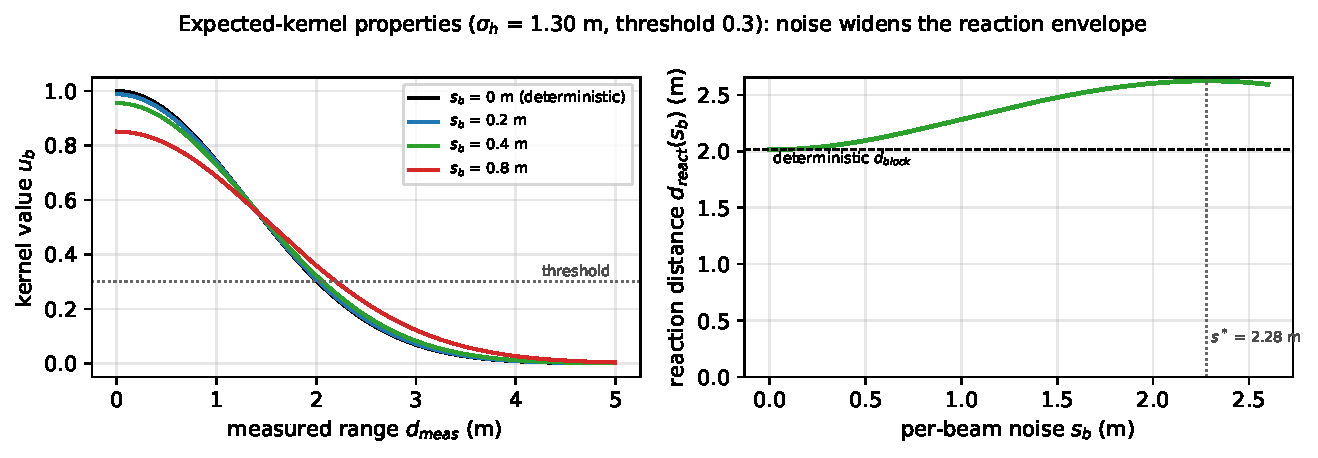
\includegraphics[width=0.92\textwidth]{figures/kernel_theory.pdf}
\caption{The expected kernel for the reference payload. Left: $u_b$ against
measured range for four noise levels; the curves cross at
$d_{\mathrm{meas}} = \sqrt{\sigma_h^2 + s_b^2}$. Right: the reaction
distance of Proposition~2.}
\label{fig:theory}
\end{figure}

\paragraph{Cost.} Per step P-VFH adds, over the deterministic histogram,
one square root and one exponential per beam for $u_b$ (and one error
function per beam for the diagnostic $p_b$): $O(n_{\mathrm{beams}})$ extra
work on top of the $O(n_{\mathrm{beams}} \cdot n_{\mathrm{obstacles}})$
raycast both share. The measured per-step compute is in
Table~\ref{tab:e1}.
Per sector, kernels compose by \textbf{max} --- the nearest-return rule, as in
the deterministic stack (kernels are not probabilities, so noisy-OR would
double-count). The two layers then flow through the same VFH+ propagation,
smoothing, threshold, valley search and hysteresis as
Section~\ref{sec:algorithms}, and the chosen valley direction is fused with
the APF obstacle reflex (computed on the same noisy scan) exactly like the
deterministic composition.

\subsection{The recursive range filter}
\label{sec:rfilter}

What the sensor model buys is knowledge of how much to trust one scan.
P-VFH keeps, for every beam $b$ of the fixed lidar fan, a scalar Bayesian
(Kalman) estimate of the range along that bearing: the true range is
modelled as a random walk with per-step standard deviation $q = 0.08$~m
(sensor and mover motion between two scans), and each scan is a
measurement with the sensor's own $s_b$:
\begin{equation}
K_b = \frac{P_b + q^2}{P_b + q^2 + s_b^2},\qquad
\hat d_b \leftarrow \hat d_b + K_b\,(d_{\mathrm{meas},b} - \hat d_b),\qquad
P_b \leftarrow (1 - K_b)(P_b + q^2).
\label{eq:rfilter}
\end{equation}
The posterior mean $\hat d_b$ and the posterior standard deviation
$\sqrt{P_b} \le s_b$ then replace $d_{\mathrm{meas},b}$ and $s_b$ in the
expected kernel~\eqref{eq:ukernel} and in the reflex. Three points:
\begin{itemize}[leftmargin=1.6em]
\item \textbf{The gain is set by the noise model, not tuned.} For a
precise sensor ($s_b \ll q$) $K_b \to 1$ and nothing is filtered, so the
deterministic limit of Proposition~1 survives; for a noisy one the filter
averages over several scans.
\item \textbf{Discontinuities are not smoothed.} An innovation larger than
three standard deviations (a beam sliding off an edge, a mover entering
the beam) re-initialises that beam to the measurement, so a newly visible
obstacle is never seen late.
\item \textbf{Scope.} The filter needs a fixed beam fan and one persistent
history, so it runs for the transport leader with the lidar; with the
body-fixed ToF fan P-VFH falls back to the single-scan kernel.
\end{itemize}
\code{'pvfh\_filt'} applies the same filter to the deterministic law, so
the grid separates what the filter contributes from what the expected
kernel contributes.

\subsection{The two APF+VFH compositions}

\begin{table}[h]
\centering
\begin{tabular}{@{}lp{6.2cm}p{6.2cm}@{}}
\toprule
 & \textbf{Phase 1 (forming)} & \textbf{Phase 2 (transport)}\\
\midrule
Architecture & \textbf{Cascaded}: APF builds a virtual goal
$\mathbf{g}_v = \mathbf{p} + \mathbf{F}$, VFH steers toward it & 
\textbf{Weighted sum}: $\theta_{\mathrm{raw}}$ from
$w_g\,\hat{\mathbf{v}}_{\mathrm{goal}} + w_v\,\hat{\mathbf{v}}_{\mathrm{vfh}}$\\
APF role & slot attraction + formation-mate repulsion & pure goal attraction
(no mates: the leader has none)\\
VFH margin & robot radius & \textbf{circumradius} $+$ robot radius\\
Speed logic & $v = V_f \min(1, e_i/r_{\mathrm{slow}})$ & $v = V \cdot
\text{speed\_scale}$ (movers)\\
\bottomrule
\end{tabular}
\caption{The same two algorithms, composed differently per phase. In
transport the goal weight is faded by the agreement between the two
directions, $w_g \max(0, \hat{\mathbf{v}}_{\mathrm{goal}} \cdot
\hat{\mathbf{v}}_{\mathrm{steer}})$: with a fixed weight a $90^\circ$ detour
chosen by the steering law is dragged back to $63^\circ$, toward the
obstacle it was avoiding (\code{cfg.blend\_fade}; not applied to
\code{'apf'}).}
\label{tab:arch}
\end{table}

\subsection{Convoy / queueing behaviour (Phase 1 only)}

Robots squeezed by a \emph{compact static} obstacle (largest footprint
$\le 2.0$~m --- pillars and pallets, never walls or shelf racks) may switch to
single-file mode: the group elects a leader, the leader leaves a trail, and
followers target points at $1.0$~m spacing along the trail
(\code{point\_along\_trail\_} \code{\allowbreak behind.m}). This trades
formation geometry for progress through a pinch, then reforms on the other
side. Movers are never convoy anchors --- the trail logic assumes a
stationary thing to queue behind.

\subsection{The safety gate, stuck escape and the anti-deadlock layer}
\label{sec:gate}

\paragraph{Atomic pose commit.} Each transport step proposes a new pose
(position \emph{and} heading). It is committed only if the whole body is
collision-free at $t$ and $t+\Delta t$. If the translation is refused, the
rotation alone is tested (a rigid frame may pivot about its centroid); if
that is refused too, the pose is held; a body held for more than five
steps makes a \emph{recovery move} --- it backs up half a step along its
axis, or turns the other way round --- because a body that can neither
advance nor rotate would otherwise hold forever. Every refusal is logged
as a \emph{gate rejection}. Because the gate uses the exact world geometry, a
committed pose is never in static contact; the rejection count is therefore
the safety metric of this report --- it counts the collisions the steering
law \emph{would} have caused without a supervisor. (Before the audit the
heading was committed without the check, so a blocked body rotated in place
into the obstacle; \S\ref{sec:audit}.) Contact can still occur from the
other side: movers are kinematic and never yield, so a mover can drive into
a body that is holding still. Those steps are counted separately as
\emph{mover contacts}.

\paragraph{Load-carrying motion limits.} The frame is a rigid payload on
$K$ robots, and a slot at distance $r_c$ from the centre moves at up to
$v + \lvert\omega\rvert r_c$. An unconstrained yaw rate therefore asks the
outer robot for speed it does not have: in a reference run without limits
a corner robot needed $3.0$~m/s while the centre drove $0.6$~m/s, with yaw
accelerations up to $13.7$~rad/s$^2$. Each step the commanded turn is
shaped, for every steering law alike: a braking curve
$\lvert\omega\rvert \le 0.8\sqrt{2\,\alpha_{\max}\lvert e_\theta\rvert}$
(never turn faster than can be stopped on the target heading); yaw rate
$\lvert\omega\rvert \le (v_{\max} - v_{\mathrm{floor}})/r_c$; yaw
acceleration $\lvert\dot\omega\rvert \le \alpha_{\max} = 2.5$~rad/s$^2$;
and speed $v \le \min\bigl(v_{\max} - \lvert\omega\rvert r_c,\;
a_{\mathrm{lat}}/\lvert\omega\rvert\bigr)$, with robot speed limit
$v_{\max} = 1.0$~m/s, lateral-acceleration limit
$a_{\mathrm{lat}} = 0.8$~m/s$^2$ and speed floor
$v_{\mathrm{floor}} = 0.5\,V$. The floor matters: a first version let the
yaw rate rise until the speed reached zero, and the formation then pivoted
in place in a mover's lane and was run into. The formation slows down to
turn, but does not stop to pivot unless the safety gate blocks its
translation. \textbf{The limits are off by default} (\code{cfg.kin}) and
evaluated as their own experiment, E14 (\S\ref{sec:e14}): the steering
stack was tuned for the agile body, and switching the limits on without
re-tuning it makes the formation slow enough to be caught by traffic. At the switch from forming to transport the
robots' residual slot error (up to the $0.3$~m forming tolerance) decays
with a $1$~s time constant rather than vanishing in one step.

\paragraph{Escape probe.} When a step is rejected repeatedly (5 consecutive times), the agent probes 36
headings sorted by deviation from the desired one and takes the first along
which the body can actually \emph{translate} one step. Two classic
implementation bugs this avoids: (i) testing the rotated body \emph{in place}
(a body blocked ahead is not itself in collision, so the probe trivially
``succeeds'' without escaping) and (ii) testing only the slot points, which a
0.8~m pillar can sit between undetected.

\paragraph{Anti-deadlock layer.} Two additions close the loop between
probing and going, identically for \emph{every} steering law: (i) a
\emph{progress window} --- $150$ steps ($15$~s) with less than $0.30$~m of
net motion along the start$\to$goal axis forces a probe even when every
step was accepted, catching stalls made of legal micro-steps; (ii)
\emph{commit-after-probe} --- a found escape heading is held for $40$ steps
(rate-limited turn, every pose still gated), and a window-triggered probe
skips headings within $0.5$~rad of the previous escape so it cannot
re-commit to the same dead end. \code{cfg.adl.enable = false} restores the
one-shot probe; E9 (\S\ref{sec:e9}) measures the difference.

\subsection{Feasibility check (run before trusting anything)}

\code{world\_feasibility.m} flood-fills a thresholded clearance grid with
bisection on the threshold to find the corridor bottleneck --- the widest
half-corridor on the best start$\to$goal path. A rigid $2\times2$ block at
spacing $s$ needs circumradius
$c = (N-1)\,s\,\sqrt{2}/2 + r$; if $c$ exceeds the bottleneck, \emph{no}
controller tuning will get the formation through, and the script either
auto-reduces $s$ or fails loudly. For the dynamic world: bottleneck
$1.22$~m, spacing used $1.18$~m, circumradius $1.01$~m, margin $0.21$~m.

\section{The dynamic-obstacle extension}
\label{sec:dynamic}

Static obstacles test avoidance; \emph{moving} obstacles test prediction. The
dynamic world adds three kinematic movers (two 0.7~m forklift-class boxes, one
1.0~m drum) driven by a shared motion contract, and the controller gains three
mechanisms to survive them.

\subsection{The shared motion contract}

Both the MATLAB simulation and the (future) ROS~2 stack evaluate obstacle
motion from one file, \code{dynamic\_obstacles.json}, interpreted by one
function (\code{eval\_mover\_pose.m}):
%
\[
\mathbf{m}(t) =
\begin{cases}
\mathbf{a} & t < t_0 \quad \text{(parked at the route start)}\\[2pt]
\mathbf{a} + \min\!\bigl(1,\, \tfrac{(t - t_0)\,v_m}{L}\bigr)(\mathbf{b} - \mathbf{a})
& \text{one-way}\\[4pt]
\text{shuttle } \mathbf{a} \leftrightarrow \mathbf{b},\ \text{leg time } 
T = \tfrac{L}{v_m} + t_{\mathrm{wait}} & \text{loop}
\end{cases}
\]
%
The velocity is piecewise constant, so \textbf{constant-velocity prediction is
exact between speed changes}, not an approximation. The scenario: mover1
crosses west$\to$east at $y = +0.5$ once (the formation yields); mover2 sweeps
the main aisle head-on forever; mover3 patrols the south aisle as background
traffic.

\subsection{Mechanism 1: predictive scan}

\code{pvfh\_predict.m} extends the VFH input: movers are raycast at their
contracted poses $t,\ t+\Delta t,\ \dots,\ t+T_{\mathrm{lead}}$
($T_{\mathrm{lead}} = 0.5$~s, sampled at $\Delta t$) and each beam keeps the
\emph{nearest blocking instance over the whole horizon}. The static sensing
path is untouched --- statics do not move, so their perception needs no
prediction. Effect: a mover closing head-on at $0.9$~m/s appears in the
histogram $\sim 0.5$~s ($\approx 0.45$~m of range) before an instantaneous
scan would place it inside the danger zone.

\begin{keybox}{A design dead end worth recording}
An earlier variant shifted the \emph{sensor position} by the self-motion
$\mathbf{v}_{\mathrm{self}} T_{\mathrm{lead}}$ and shortened all beams by the
self-displacement. That couples the current heading into the perception of
\emph{static} geometry: the controller sees different walls depending on which
way it points, and the feedback loop produces heading limit cycles. The fix
was architectural --- predict only the things that move. It is a good example
of why per-module numerics (scan construction) matter more than gains.
\end{keybox}

\subsection{Mechanism 2: speed slowdown}

The transport speed scales down smoothly as the \emph{predicted} worst-case
gap to any mover shrinks:
%
\begin{align*}
\text{speed\_scale} &=
\begin{cases}
\max\bigl(s_{\min},\ 0.8\, g_{\mathrm{pred}} / (m_{\mathrm{slow}} + r)\bigr)
& g_{\mathrm{pred}} < m_{\mathrm{slow}} + r\\
1 & \text{otherwise}
\end{cases}\\[6pt]
g_{\mathrm{pred}} &= \min_{T \le T_{\mathrm{look}}}
\Bigl[ \lVert \mathbf{m}(t{+}T) - \mathbf{c} - \mathbf{v}_{\mathrm{self}} T \rVert
- r_m - \lVert \mathbf{v}_{\mathrm{self}}\rVert T \Bigr]
\end{align*}
%
with $m_{\mathrm{slow}} = 0.25$~m, $s_{\min} = 0.4$, $T_{\mathrm{look}} =
1.0$~s. The floor $s_{\min}$ keeps the formation making progress (a full stop
near a moving obstacle is how deadlocks form); movers slower than 25\% of the
formation's speed are treated as parked and do not trigger the slowdown.

\subsection{Mechanism 3: the $t$ and $t{+}\Delta t$ commit test}

A step is committed only if the whole body (payload block included, via the
exact separating-axis test) is collision-free at $t$ \emph{and} at
$t + \Delta t$ with the movers at their contracted future poses. This is what
stops the block from stepping into a lane a forklift occupies one tick later.
The escape probe got the matching treatment: an escape heading is accepted
only if the body can hold it for $T_{\mathrm{hold}} = 1.5$~s while the movers
keep moving.

\subsection{Verified outcome}

(Single reference run recorded \emph{before} the October 2026 audit of
\S\ref{sec:audit}; re-run \code{Simulation8\_dynamic} to refresh it --- the
Monte Carlo tables of \S\ref{sec:experiments} are the authoritative
numbers.) On the dynamic world the full pipeline reaches the goal with
\textbf{zero collision steps}, minimum formation clearance $0.51$~m, minimum
gap to any mover $1.22$~m (the predicted worst case $0.33$~m, absorbed by the
slowdown and VFH), path efficiency $0.93$, total turning $12.0$~rad over
$42.5$~s of transport. The static-world regression on the same parameters is
unchanged, confirming the dynamic layer costs nothing when nothing moves.

\section{Control flow}

\subsection{System overview}

\begin{figure}[H]
\centering
\resizebox{\textwidth}{!}{%
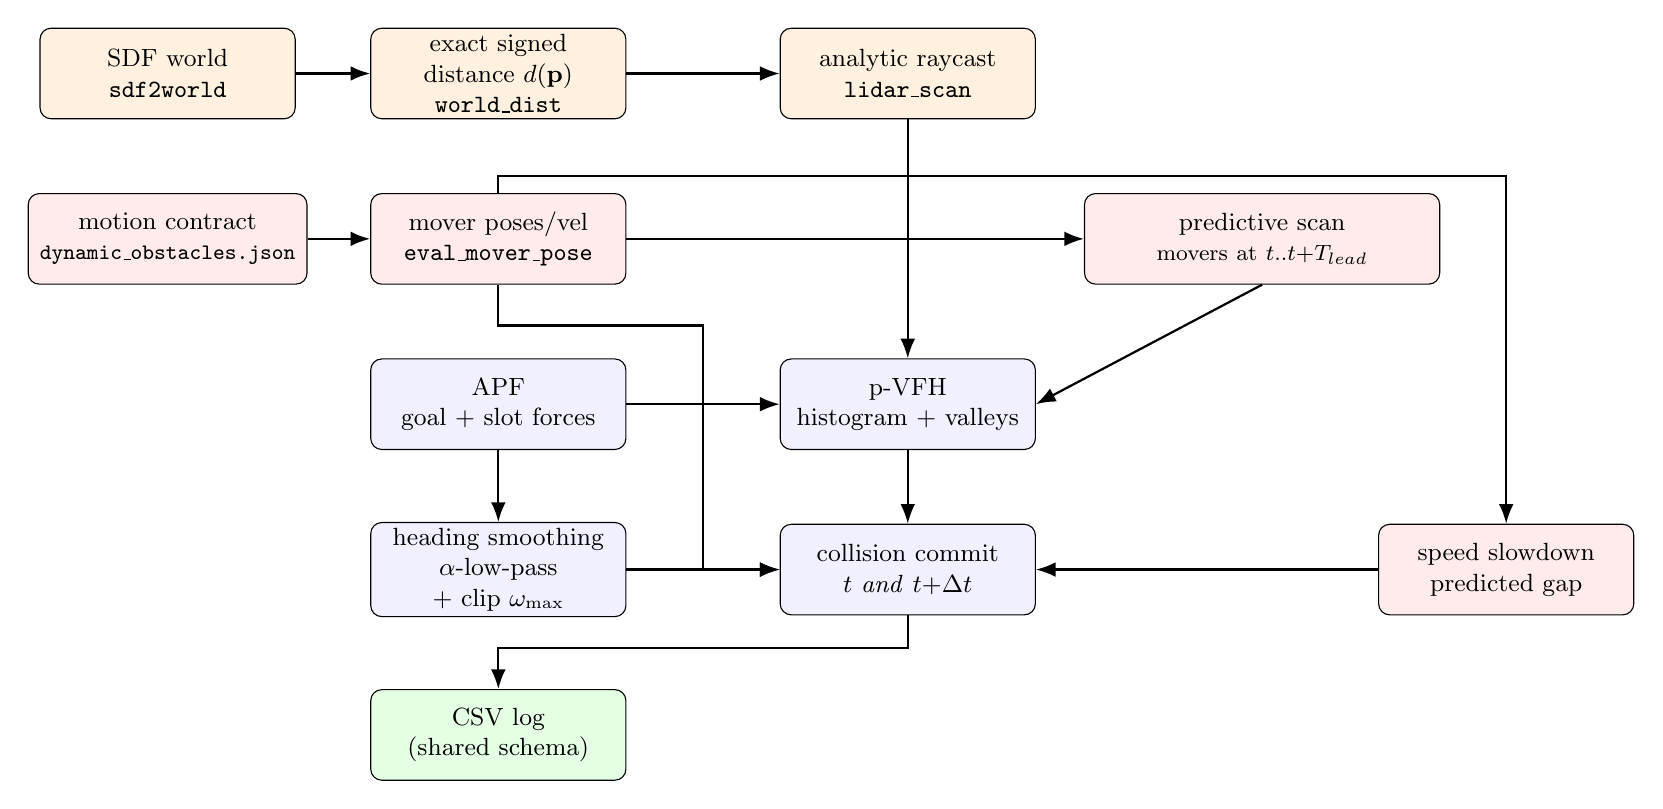
\begin{tikzpicture}[
  box/.style={draw, rounded corners, fill=blue!6, text width=3.1cm,
              minimum height=1.15cm, align=center, font=\small, inner sep=2pt},
  geo/.style={box, fill=orange!12},
  dyn/.style={box, fill=red!8},
  io/.style={box, fill=green!10},
  arr/.style={-{Latex[length=2.5mm]}, thick}
]
% row 0: geometry pipeline
\node[geo] (sdf) at (0,0) {SDF world\\ \code{sdf2world}};
\node[geo] (sd) at (4.2,0) {exact signed distance $d(\mathbf{p})$\\ \code{world\_dist}};
\node[geo] (lidar) at (9.4,0) {analytic raycast\\ \code{lidar\_scan}};
% row 1: dynamic-obstacle pipeline
\node[dyn, text width=3.4cm] (json) at (0,-2.1) {motion contract\\ \footnotesize\code{dynamic\_obstacles.json}};
\node[dyn] (movers) at (4.2,-2.1) {mover poses/vel\\ \code{eval\_mover\_pose}};
\node[dyn, text width=4.3cm, inner sep=3pt] (pred) at (13.9,-2.1) {predictive scan\\ \footnotesize movers at $t..t{+}T_{lead}$};
% row 2: fusion into avoidance
\node[box] (apf) at (4.2,-4.2) {APF\\ goal + slot forces};
\node[box] (vfh) at (9.4,-4.2) {p-VFH\\ histogram + valleys};
% row 3: control finishing + commit
\node[box] (smooth) at (4.2,-6.3) {heading smoothing\\ $\alpha$-low-pass + clip $\omega_{\max}$};
\node[box] (commit) at (9.4,-6.3) {collision commit\\ $t$ \emph{and} $t{+}\Delta t$};
\node[dyn] (slow) at (17.0,-6.3) {speed slowdown\\ predicted gap};
% row 4: output
\node[io] (log) at (4.2,-8.4) {CSV log\\ (shared schema)};

% row 0 chain
\draw[arr] (sdf) -- (sd);
\draw[arr] (sd) -- (lidar);
% row 1 chain
\draw[arr] (json) -- (movers);
\draw[arr] (movers) -- (pred);
% vertical links row0 -> row2 (clear column, x=9.4)
\draw[arr] (lidar.south) -- (vfh.north);
% pred -> vfh (short diagonal, row1 col3 -> row2 col2)
\draw[arr] (pred.south) -- (vfh.east);
% row 2 chain
\draw[arr] (apf) -- (vfh);
% row2 -> row3
\draw[arr] (vfh.south) -- (commit.north);
\draw[arr] (apf.south) -- (smooth.north);
% row 3 chain
\draw[arr] (smooth) -- (commit);
\draw[arr] (slow) -- (commit);
% movers -> commit, routed through the empty channel at x=6.8 (clear of the
% apf--vfh and smooth--commit arrows, which end at x=5.75 / start at x=7.85)
\draw[arr] (movers.south) -- (4.2,-3.2) -- (6.8,-3.2) -- (6.8,-6.3) -- (commit.west);
% movers -> slow, routed above row 1 then down the far right-hand column
% (x=17.0, clear of the "predictive scan" box, which ends at x=16.05)
\draw[arr] (movers.north) -- (4.2,-1.3) -- (17.0,-1.3) -- (17.0,-2.8) -- (slow.north);
% row3 -> row4
\draw[arr] (commit.south) -- (9.4,-7.3) -- (4.2,-7.3) -- (log.north);
\end{tikzpicture}%
}
\caption{Data flow of the whole stack. Orange: world/geometry. Blue: the
control path. Red: dynamic-obstacle inputs. Every box is one self-contained
file, testable in isolation.}
\end{figure}

\subsection{Phase 1 --- forming up (per robot, per tick)}

\begin{figure}[H]
\centering
\resizebox{0.82\textwidth}{!}{%
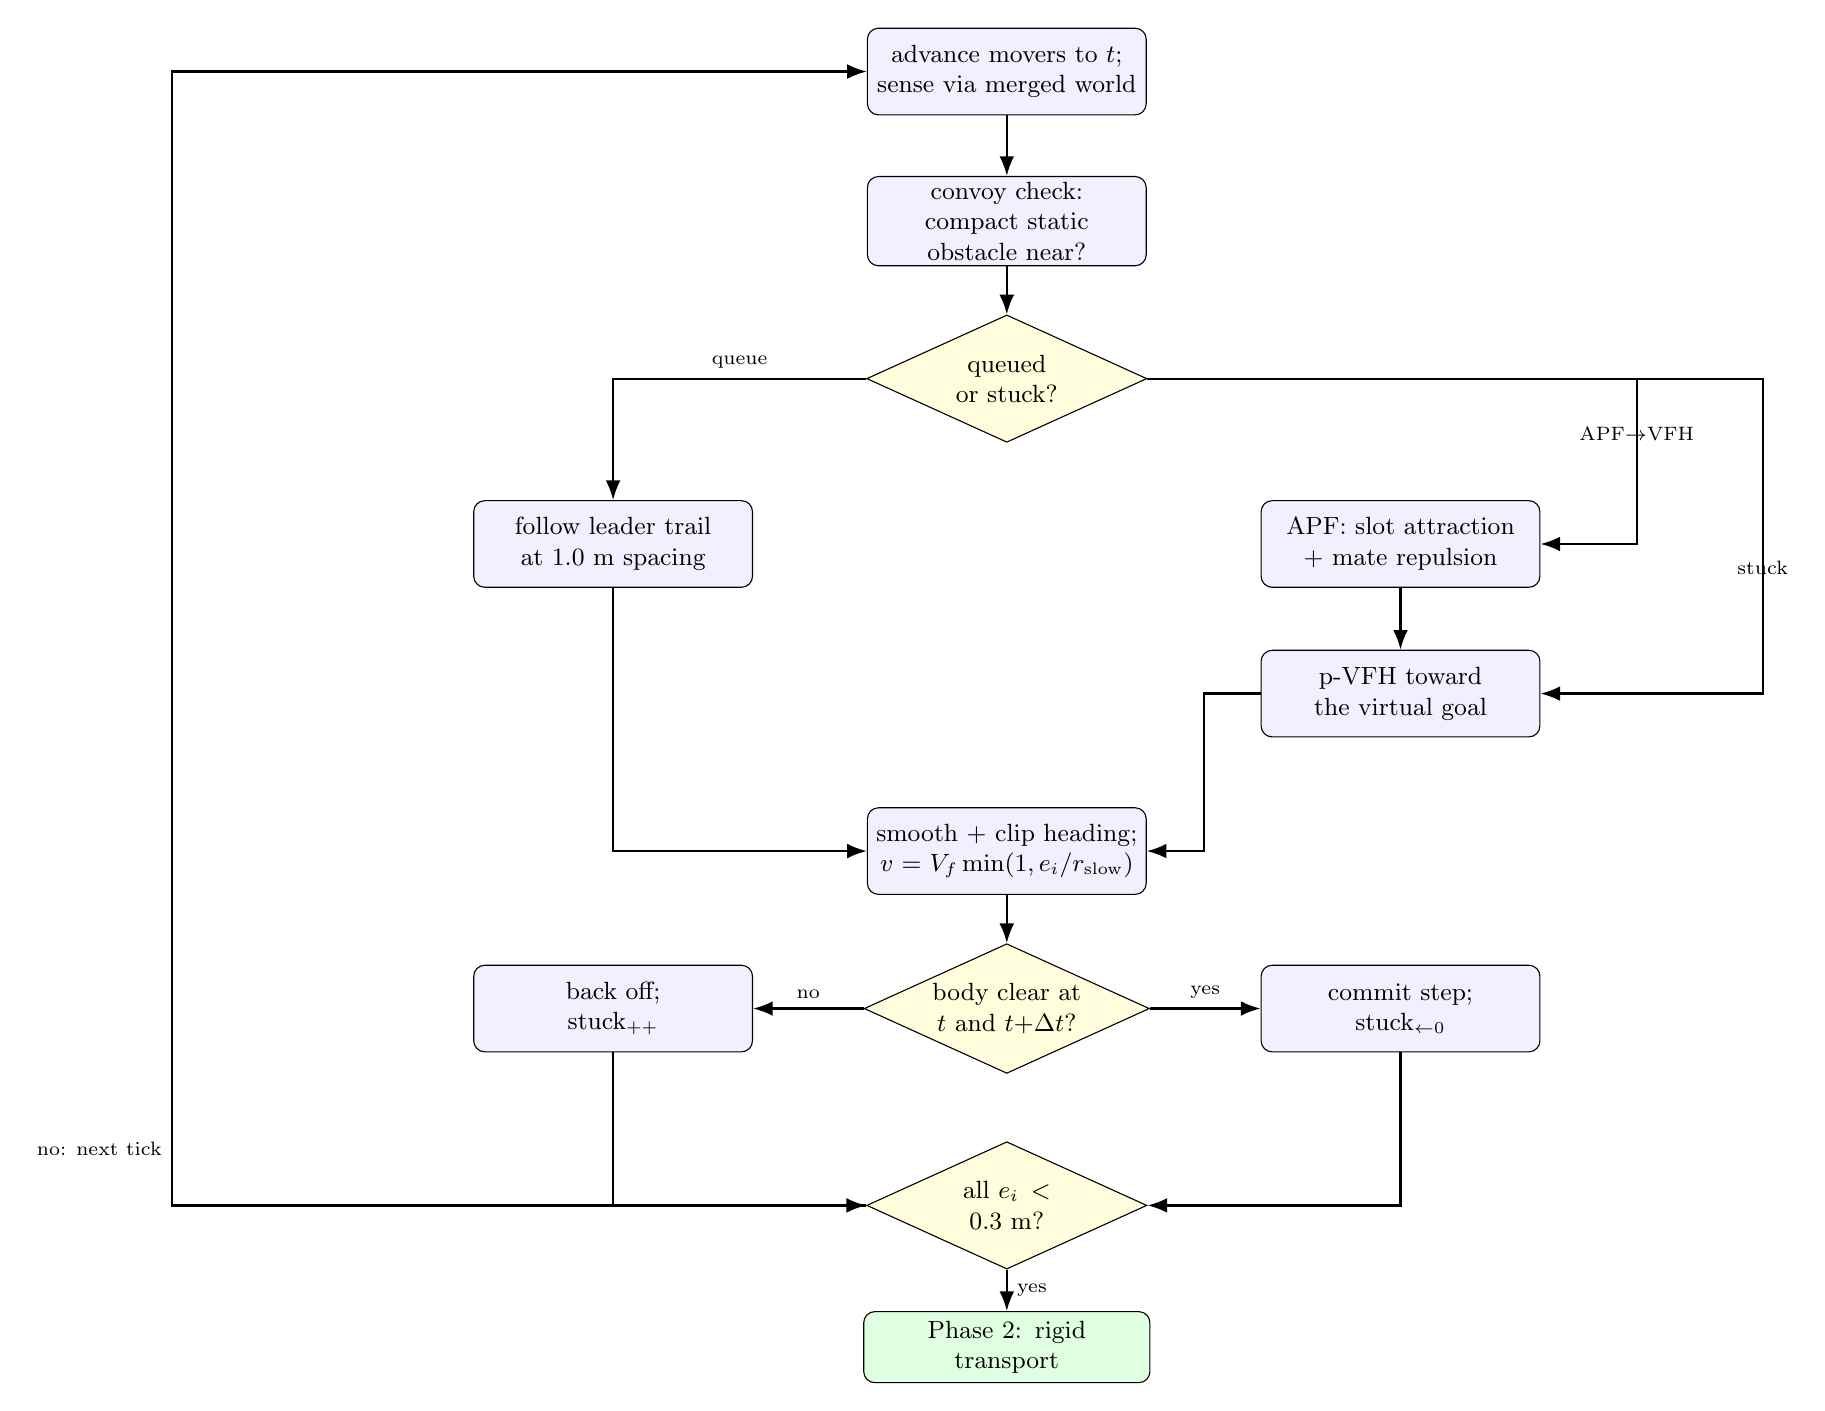
\begin{tikzpicture}[
  procbox/.style={draw, rounded corners, fill=blue!6, text width=3.4cm,
               minimum height=1.1cm, align=center, font=\small, inner sep=2pt},
  dec/.style={draw, diamond, aspect=2.2, fill=yellow!14, align=center,
              font=\small, inner sep=1pt, text width=2.0cm},
  arr/.style={-{Latex[length=2.5mm]}, thick},
  term/.style={draw, rounded corners, fill=green!12, minimum height=0.9cm,
               text width=3.4cm, align=center, font=\small}
]
\node[procbox] (sense) at (8,0)     {advance movers to $t$;\\ sense via merged world};
\node[procbox] (conv)  at (8,-1.9)  {convoy check:\\ compact static obstacle near?};
\node[dec]  (mode)  at (8,-3.9)  {queued or stuck?};
\node[procbox] (trail) at (3,-6.0)  {follow leader trail\\ at 1.0 m spacing};
\node[procbox] (apf)   at (13,-6.0) {APF: slot attraction\\ + mate repulsion};
\node[procbox] (vfh)   at (13,-7.9) {p-VFH toward\\ the virtual goal};
\node[procbox] (ctrl)  at (8,-9.9)  {smooth + clip heading;\\ $v = V_f\min(1, e_i/r_{\mathrm{slow}})$};
\node[dec]  (safe)  at (8,-11.9) {body clear at\\ $t$ and $t{+}\Delta t$?};
\node[procbox] (back)  at (3,-11.9) {back off;\\ stuck$_{++}$};
\node[procbox] (go)    at (13,-11.9){commit step;\\ stuck$_{\leftarrow 0}$};
\node[dec]  (formed) at (8,-14.4) {all $e_i < 0.3$ m?};
\node[term] (out)   at (8,-16.2) {Phase 2: rigid transport};

\draw[arr] (sense) -- (conv);
\draw[arr] (conv) -- (mode);
\draw[arr] (mode.west) -| node[above,pos=0.25,font=\scriptsize]{queue} (trail.north);
\draw[arr] (mode.east) -- (16,-3.9) -- (16,-6.0) -- (apf.east);
\node[font=\scriptsize] at (16,-4.6) {APF$\to$VFH};
\draw[arr] (mode.east) -- (17.6,-3.9) -- (17.6,-7.9) -- (vfh.east);
\node[font=\scriptsize] at (17.6,-6.3) {stuck};
\draw[arr] (trail.south) -- (3,-9.9) -- (ctrl.west);
\draw[arr] (apf) -- (vfh);
\draw[arr] (vfh.west) -- (10.5,-7.9) -- (10.5,-9.9) -- (ctrl.east);
\draw[arr] (ctrl) -- (safe);
\draw[arr] (safe.west) -- node[above,font=\scriptsize]{no} (back.east);
\draw[arr] (safe.east) -- node[above,font=\scriptsize]{yes} (go.west);
\draw[arr] (back.south) -- (3,-14.4) -- (formed.west);
\draw[arr] (go.south) -- (13,-14.4) -- (formed.east);
\draw[arr] (formed) -- node[right,font=\scriptsize]{yes} (out);
\draw[arr] (formed.west) -- (-2.6,-14.4) -- node[left,pos=0.05,font=\scriptsize]{no: next tick} (-2.6,0) -- (sense.west);
\end{tikzpicture}%
}
\caption{Phase 1. Each robot runs this independently; the only coupling is
the repulsion between formation mates and the convoy grouping.}
\end{figure}

\subsection{Phase 2 --- rigid transport (one virtual leader)}

\begin{figure}[H]
\centering
\resizebox{0.82\textwidth}{!}{%
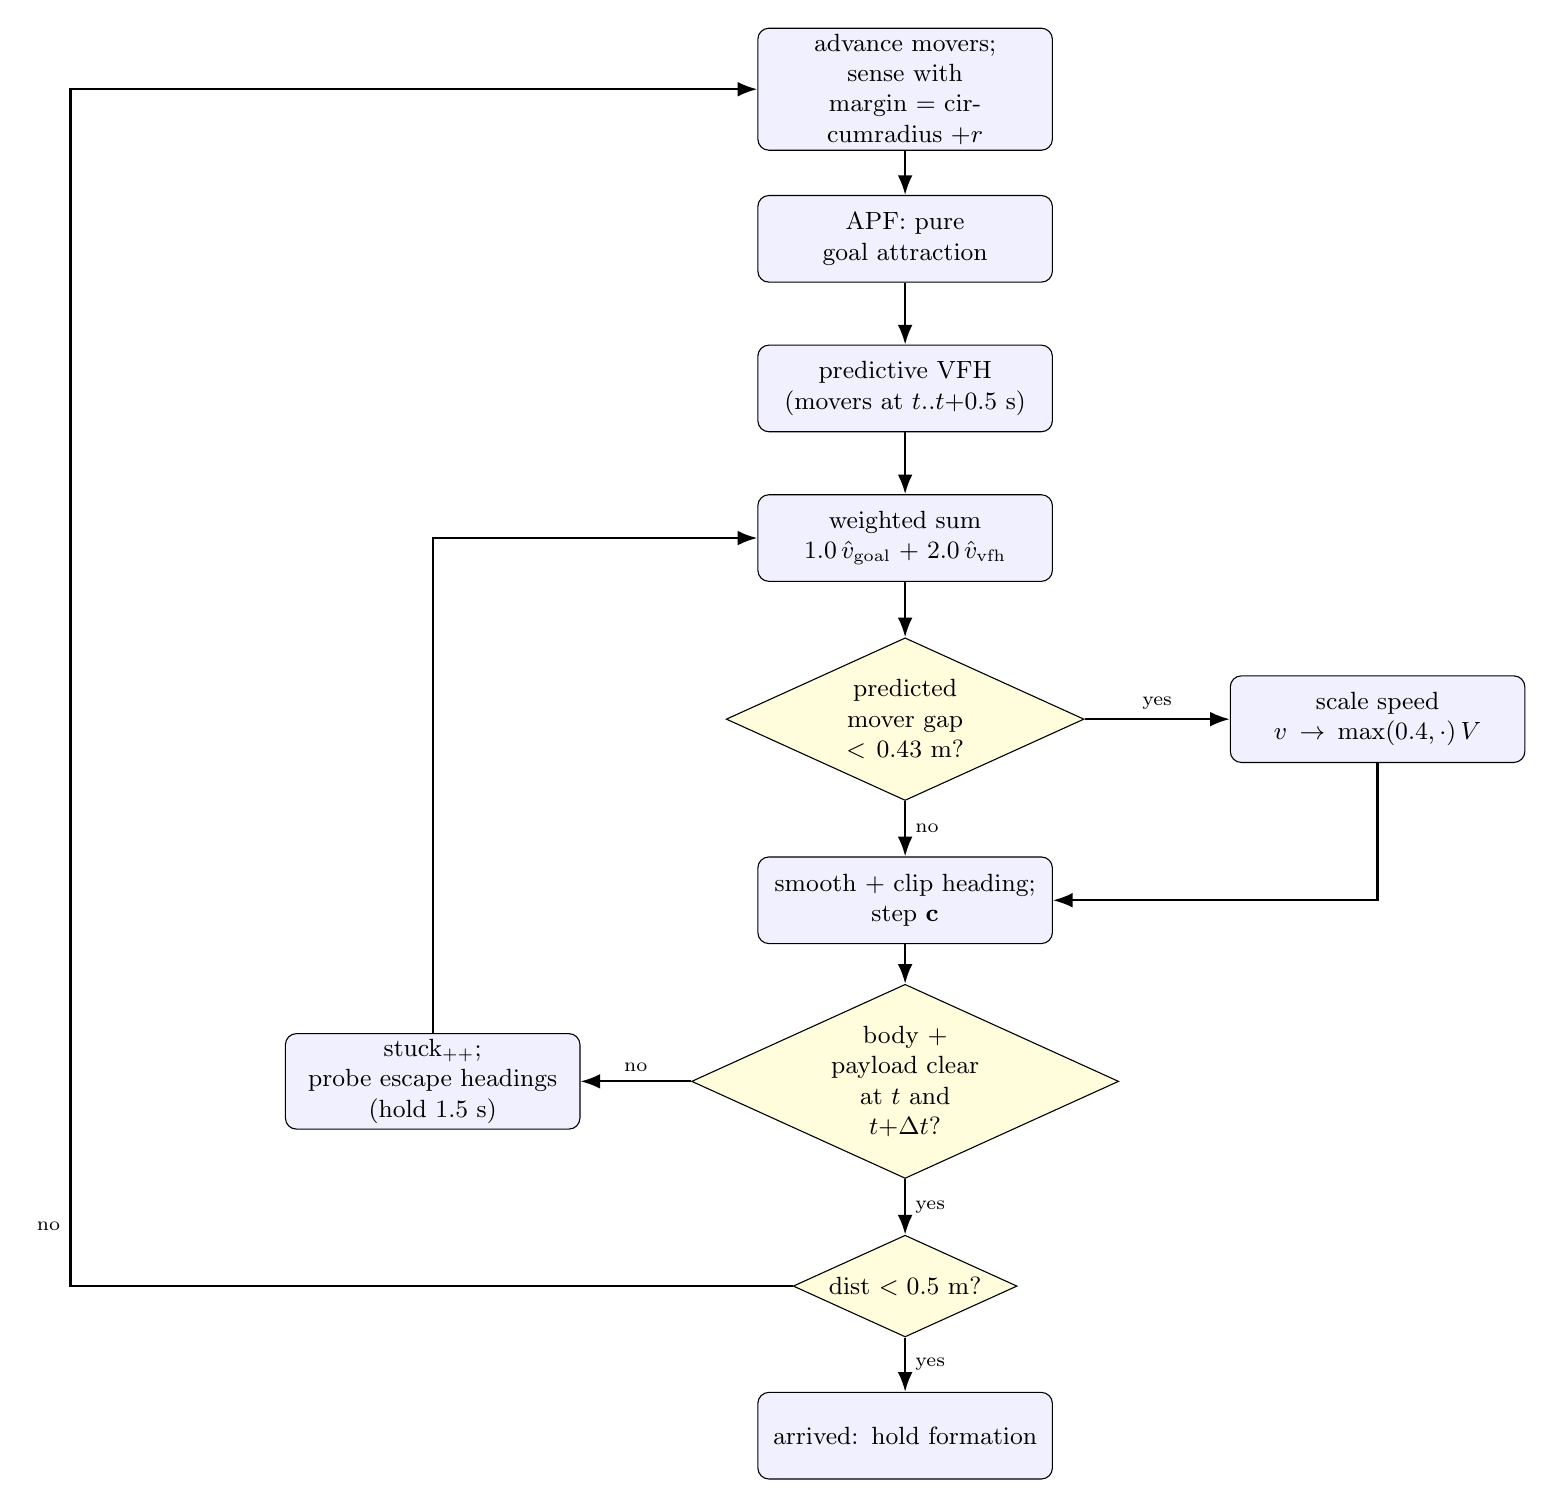
\begin{tikzpicture}[
  procbox/.style={draw, rounded corners, fill=blue!6, text width=3.6cm,
               minimum height=1.1cm, align=center, font=\small, inner sep=2pt},
  dec/.style={draw, diamond, aspect=2.2, fill=yellow!14, align=center,
              font=\small, inner sep=1pt, text width=2.1cm},
  arr/.style={-{Latex[length=2.5mm]}, thick}
]
\node[procbox] (sense) at (8,0)     {advance movers; sense with\\ margin $=$ circumradius $+ r$};
\node[procbox] (apf)   at (8,-1.9)  {APF: pure goal attraction};
\node[procbox] (vfh)   at (8,-3.8)  {predictive VFH\\ (movers at $t..t{+}0.5$ s)};
\node[procbox] (blend) at (8,-5.7)  {weighted sum\\ $1.0\,\hat v_{\mathrm{goal}} + 2.0\,\hat v_{\mathrm{vfh}}$};
\node[dec]  (gap)   at (8,-8.0)  {predicted mover gap $< 0.43$ m?};
\node[procbox] (slow)  at (14,-8.0) {scale speed\\ $v \to \max(0.4, \cdot)\,V$};
\node[procbox] (ctrl)  at (8,-10.3) {smooth + clip heading;\\ step $\mathbf{c}$};
\node[dec]  (safe)  at (8,-12.6) {body + payload clear\\ at $t$ and $t{+}\Delta t$?};
\node[procbox] (stuck) at (2,-12.6) {stuck$_{++}$;\\ probe escape headings\\ (hold 1.5 s)};
\node[dec]  (goal)  at (8,-15.2) {dist $< 0.5$ m?};
\node[procbox] (done)  at (8,-17.1) {arrived: hold formation};

\draw[arr] (sense) -- (apf);
\draw[arr] (apf) -- (vfh);
\draw[arr] (vfh) -- (blend);
\draw[arr] (blend) -- (gap);
\draw[arr] (gap.east) -- node[above,font=\scriptsize]{yes} (slow.west);
\draw[arr] (slow.south) -- (14,-10.3) -- (ctrl.east);
\draw[arr] (gap.south) -- node[right,font=\scriptsize]{no} (ctrl.north);
\draw[arr] (ctrl) -- (safe);
\draw[arr] (safe.west) -- node[above,font=\scriptsize]{no} (stuck.east);
\draw[arr] (stuck.north) -- (2,-5.7) -- (blend.west);
\draw[arr] (safe.south) -- node[right,font=\scriptsize]{yes} (goal.north);
\draw[arr] (goal.south) -- node[right,font=\scriptsize]{yes} (done.north);
\draw[arr] (goal.west) -- (-2.6,-15.2) -- node[left,pos=0.05,font=\scriptsize]{no} (-2.6,0) -- (sense.west);
\end{tikzpicture}%
}
\caption{Phase 2. The four robots then servo to their slots of the frame
$(\mathbf{c}, \theta)$; in the kinematic model this is exact, in ROS~2 it is
a real controller whose residual is the formation error.}
\end{figure}

\subsection{P-VFH data flow (the probabilistic variant)}
\label{sec:pvfhflow}

\begin{figure}[H]
\centering
\resizebox{\textwidth}{!}{%
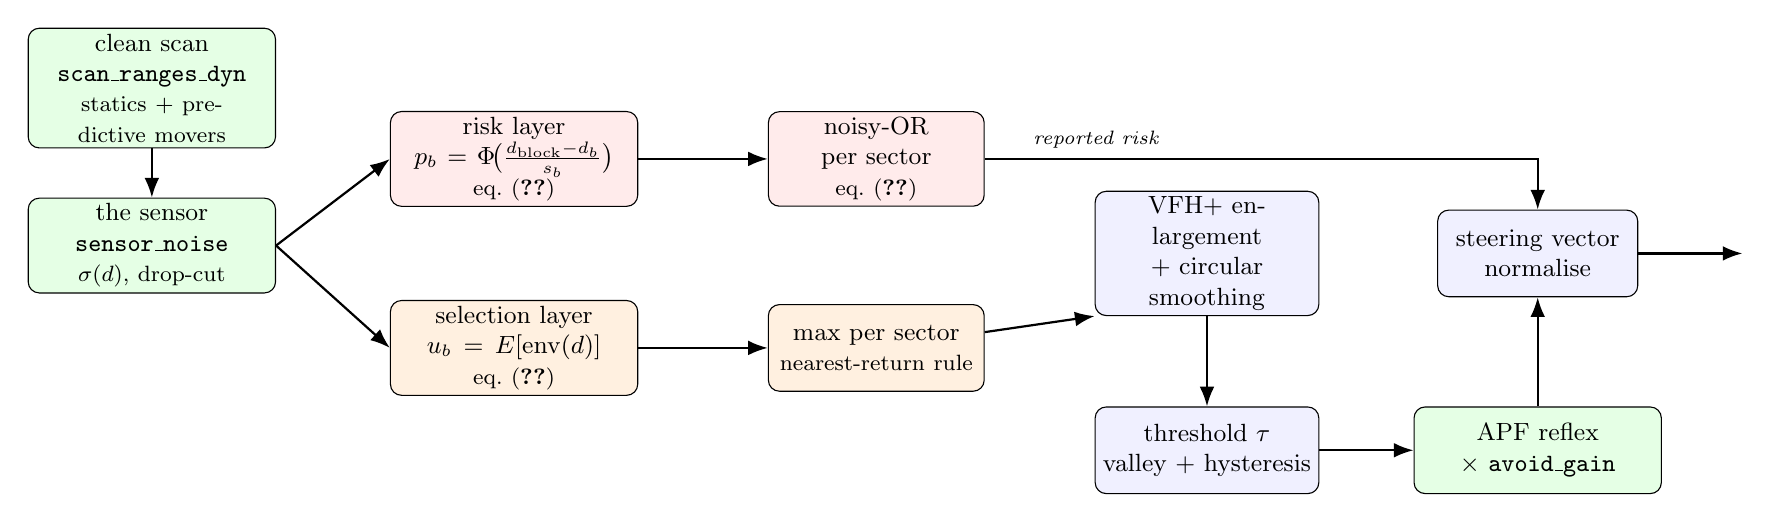
\begin{tikzpicture}[
  box/.style={draw, rounded corners, fill=blue!6, text width=3.0cm,
              minimum height=1.1cm, align=center, font=\small, inner sep=2pt},
  risk/.style={box, fill=red!8},
  sel/.style={box, fill=orange!12},
  shared/.style={box, fill=green!10},
  arr/.style={-{Latex[length=2.5mm]}, thick}
]
% shared front end
\node[shared] (scan) at (0,0) {clean scan\\ \code{scan\_ranges\_dyn}\\ \footnotesize statics + predictive movers};
\node[shared] (noise) at (0,-2.0) {the sensor\\ \code{sensor\_noise}\\ \footnotesize $\sigma(d)$, drop-cut};
% two per-beam layers
\node[risk] (probl) at (4.6,-0.9) {risk layer\\ $p_b=\Phi\!\bigl(\frac{d_{\mathrm{block}}-d_b}{s_b}\bigr)$\\ \footnotesize eq.~\eqref{eq:prise}};
\node[sel]  (kern)  at (4.6,-3.3) {selection layer\\ $u_b=E[\mathrm{env}(d)]$\\ \footnotesize eq.~\eqref{eq:ukernel}};
% pooling
\node[risk, text width=2.6cm] (orpool) at (9.2,-0.9) {noisy-OR per sector\\ \footnotesize eq.~\eqref{eq:noisyor}};
\node[sel, text width=2.6cm] (maxpool) at (9.2,-3.3) {max per sector\\ \footnotesize nearest-return rule};
% shared back end
\node[box, text width=2.7cm] (vfhplus) at (13.4,-2.1) {VFH+ enlargement\\ $+$ circular smoothing};
\node[box, text width=2.7cm] (valley) at (13.4,-4.6) {threshold $\tau$\\ valley $+$ hysteresis};
\node[shared] (reflex) at (17.6,-4.6) {APF reflex\\ $\times$ \code{avoid\_gain}};
\node[box, text width=2.4cm] (out) at (17.6,-2.1) {steering vector\\ normalise};
% edges
\draw[arr] (scan) -- (noise);
\draw[arr] (noise.east) -- (probl.west);
\draw[arr] (noise.east) -- (kern.west);
\draw[arr] (probl) -- (orpool);
\draw[arr] (kern) -- (maxpool);
\draw[arr] (orpool.east) -- node[above,font=\scriptsize\itshape]{reported risk} (13.4,-0.9) -| (out.north);
\draw[arr] (maxpool) -- (vfhplus.south west);
\draw[arr] (vfhplus) -- (valley);
\draw[arr] (valley) -- (reflex.west);
\draw[arr] (reflex.north) -- (out.south);
\draw[arr] (out) -- ++(2.6,0);
\end{tikzpicture}%
}
\caption{P-VFH (\code{pvfh\_prob.m}). One noisy scan feeds two per-beam layers:
the blockage probability (risk, reported and floored at $p_{\mathrm{unknown}}$)
and the posterior-expected kernel (selection, actually thresholded). The
deterministic stack is this diagram with the top branch removed and
$\mathrm{env}(d_{\mathrm{meas}})$ in place of $u_b$.}
\label{fig:pvfhflow}
\end{figure}

\section{Every parameter, and why it has that value}

\subsection{Motion and geometry}

\begin{table}[H]
\centering
\small
\begin{tabular}{@{}lllp{5.2cm}@{}}
\toprule
\textbf{Parameter} & \textbf{Value} & \textbf{Where} & \textbf{Role / why}\\
\midrule
$\Delta t$ (\code{dt}) & 0.1 s & 10 Hz & control period; also the mover
prediction sample step\\
\code{robot\_radius} & 0.18 m & all collision tests & TurtleBot3-class
footprint; feeds inflation, feasibility, VFH enlargement\\
\code{grid\_size} & $2\times2$ & formation & 4 robots; the payload block spans
the square\\
\code{grid\_spacing} & 1.18 m & slots & set by the corridor bottleneck
(feasibility check); \textbf{must match} any ROS~2 run\\
$V$ & 0.6 m/s & transport speed & fast enough to be useful, slow enough that
$T_{\mathrm{lead}}$ prediction stays valid\\
$V_f$ & 0.5 m/s & forming speed & slower assembly for gentler
slot convergence\\
$\omega_{\max}$ & 0.3 / 0.5 rad/s & transport / forming & hard turn-rate clip;
the transport value keeps the payload rotation gentle\\
$\alpha$ & 0.35 & heading smoothing & payload comfort vs obstacle reactivity
(Section~1.1)\\
\bottomrule
\end{tabular}
\end{table}

\subsection{APF gains}

\begin{table}[H]
\centering
\small
\begin{tabular}{@{}lllp{5.2cm}@{}}
\toprule
\textbf{Parameter} & \textbf{Value} & \textbf{Where} & \textbf{Role / why}\\
\midrule
\code{w\_slot} & 2.0 & Phase 1 attraction & dominant over repulsion: reaching
the slot is the objective\\
\code{w\_repulse} & 1.5 & Phase 1 mate repulsion & strong enough to prevent
overlap, weak enough not to fight the slot pull\\
\code{repulse\_dist} & 1.2 m & Phase 1 & $\approx 3\times$ robot radius; beyond
it mates do not interact\\
\code{slow\_radius} & 1.5 m & Phase 1 & linear approach deceleration
$v = V_f \min(1, e_i/r)$\\
\code{w\_goal} & 1.0 & Phase 2 blend & goal term weight\\
\code{w\_vfh} & 2.0 & Phase 2 blend & avoidance dominates: a 4 m-wide rigid
body cannot trade clearance for progress\\
\bottomrule
\end{tabular}
\end{table}

\subsection{p-VFH}

\begin{table}[H]
\centering
\small
\begin{tabular}{@{}lllp{5.0cm}@{}}
\toprule
\textbf{Parameter} & \textbf{Value} & \textbf{Where} & \textbf{Role / why}\\
\midrule
\code{n\_beams} & 288 & scan & match your LiDAR; ROS~2 default here\\
\code{num\_sectors} & 72 & histogram & $5^\circ$ resolution\\
\code{sense\_range\_base} & 4.0 m & scan range & $+$ margin (body circumradius)\\
\code{danger\_dist\_base} & 1.2 m & close reflex & NOT 2.5: in a 10 m aisle
2.5 m sees both walls, they nearly cancel, residue fights the goal term\\
\code{threshold} $\tau$ & 0.3 & valley cut & also drives $\sigma$
auto-derivation\\
\code{react\_gap} & 1.0 m & auto-$\sigma$ & reaction distance beyond the body
$r_{\mathrm{eff}} + 1.0$\\
\code{turn\_limit} & $45^\circ$ & valley search & how far off the goal bearing
the controller will look\\
\code{smooth\_window} & 5 & histogram & circular smoothing (wraps $\pm\pi$)\\
\code{avoid\_gain} & 5 & close reflex & gain of the $1/d^3$ repulsion\\
\code{hysteresis\_weight} & 0.6 & valley cost & damps sector-to-sector
heading chatter\\
\code{avoid\_falloff\_power} & 3 & close reflex & sharp near-field
dominance\\
\code{enlarge} & true & VFH+ & body-aware bearing blocking
$\gamma = \arcsin(r_{\mathrm{eff}}/d)$\\
\code{auto\_sigma} & true & histogram & $\sigma$ from required clearance, not
fixed\\
\bottomrule
\end{tabular}
\end{table}

\subsection{Algorithm axis and sensor noise}

\begin{table}[H]
\centering
\small
\begin{tabular}{@{}lllp{5.0cm}@{}}
\toprule
\textbf{Parameter} & \textbf{Value} & \textbf{Where} & \textbf{Role / why}\\
\midrule
\code{algo} & \code{'pvfh'} & both phases & the steering law:
\code{'apf'} / \code{'vfh'} / \code{'pvfh'} / \code{'pvfh\_prob'} (Section
\ref{sec:fourvariants}); all consume the same noisy scan\\
\code{p\_unknown} & 0.05 & \code{pvfh\_prob} & floor for unobserved sectors
and max-range drop-cuts: below $\tau$, so unknown space never blocks by
itself\\
\code{sense.kind} & \code{'lidar'} & \code{sensor\_noise} & or
\code{'tof'}: FoV arc of \code{fov\_deg} centred on the body heading (\code{sense.frame = 'body'}; \code{'world'} restores the legacy world-$+x$ fan)\\
\code{sigma0} & 0.02 m & \code{sensor\_noise} & base range noise; E2 sweeps
this to 0.40\\
\code{k\_rng} & 0.03 & \code{sensor\_noise} & tof distance-dependent term:
$\sigma(d) = \sigma_0 + k_{\mathrm{rng}} d$\\
\code{max\_range} & $\infty$ & drop-cut & returns at/above it report it and
are floored at \code{p\_unknown} in P-VFH\\
\code{seed} & $[]$ / 7 & PRNG & $[]$ $=$ nondeterministic; a fixed seed makes
a whole experiment reproducible\\
\bottomrule
\end{tabular}
\end{table}

\subsection{Dynamic-obstacle reaction}

\begin{table}[H]
\centering
\small
\begin{tabular}{@{}lllp{5.0cm}@{}}
\toprule
\textbf{Parameter} & \textbf{Value} & \textbf{Where} & \textbf{Role / why}\\
\midrule
\code{pred\_lead} & 0.5 s & predictive scan & horizon; with movers at
$\le 0.9$ m/s this sees $\sim 0.45$ m of approach early\\
\code{slow\_margin} & 0.25 m & slowdown & predicted gap below
$0.25 + r$ starts the speed scale\\
\code{slow\_min} & 0.4 & slowdown floor & never fully stop --- deadlocks form
at zero speed\\
\code{lookahead} & 1.0 s & worst-case gap & horizon of the slowdown metric\\
\code{avoid\_vel\_frac} & 0.25 & parked filter & movers slower than a quarter
of $V$ are static obstacles, not traffic\\
\code{hold\_time} & 1.5 s & escape probe & an escape pose must stay clear
while movers advance through it\\
\bottomrule
\end{tabular}
\end{table}

\subsection{Convoy (Phase 1)}

\begin{table}[H]
\centering
\small
\begin{tabular}{@{}lllp{5.0cm}@{}}
\toprule
\textbf{Parameter} & \textbf{Value} & \textbf{Where} & \textbf{Role / why}\\
\midrule
\code{convoy\_trigger\_dist} & 2.0 m & grouping & near enough to matter\\
\code{convoy\_exit\_dist} & 3.0 m & hysteresis & prevents mode chatter at the
trigger boundary\\
\code{convoy\_max\_obstacle} & 2.0 m & gate & only compact obstacles (pillars,
pallets) queue; walls/shelves never\\
\code{convoy\_min\_group} & 2 & grouping & one robot alone should not switch
mode\\
\code{convoy\_spacing} & 1.0 m & trail-follow & single-file gap\\
\code{tolerance} & 0.3 m & formed? & slot error that declares Phase 1 done\\
\bottomrule
\end{tabular}
\end{table}

\begin{keybox}{The one rule about parameters}
Every value above is part of the \emph{experiment definition}, not an
implementation detail. A ROS~2 replication that changes any of them is no
longer measuring the same thing; \code{compare\_runs.m} will happily produce
numbers for a meaningless comparison. The single source for the ROS~2 side is
\code{params/swarm.yaml} in the ROS~2 bundle.
\end{keybox}

\section{The graphs, and how to read them}

All figures below are generated from the verified dynamic-world run
(\code{logs/matlab\_dynamic.csv}) by \code{make\_figures.m}.

\subsection{Reading the gaps in the data first}

Every logged series has places where it legitimately carries \emph{no}
information. Plotting those samples as if they were data produces artefacts
that look like controller behaviour but are not. Three distinct kinds:

\begin{enumerate}[leftmargin=1.9em]
\item \textbf{Sentinel gaps (value $= 99$).} A column holds 99 where the
quantity is undefined --- historically ``no mover nearby''. These are
\emph{masked} to NaN by \code{make\_figures.m} so they are simply not drawn;
unmasked, a single sentinel turns a 0--10~m axis into a 0--99 axis and
everything real becomes invisible.
\item \textbf{Semantic gaps (same column, different quantity).}
\code{dist\_to\_goal} is the \emph{max slot error} during forming (converges
to 0.3 m) and the \emph{centroid-to-goal distance} during transport (starts
at 23.9 m, converges to 0.5 m). Joined into one line, the phase boundary
shows a fake jump of $0.3 \to 23.9$~m. The figures therefore draw the two
phases as separate coloured segments with a marked boundary.
\item \textbf{Coverage gaps (metric defined only in one phase).} The
predicted mover gap was originally computed only in Phase~2 (Phase~1 logs
held a 99 placeholder), so its series started mid-run with a cliff. The
current instrument computes the same per-robot prediction during forming
too, so the metric is defined across the whole run; the value is large
(3.5~m) there because the scattered robots simply are not near movers yet.
\end{enumerate}

\begin{figure}[h]
\centering
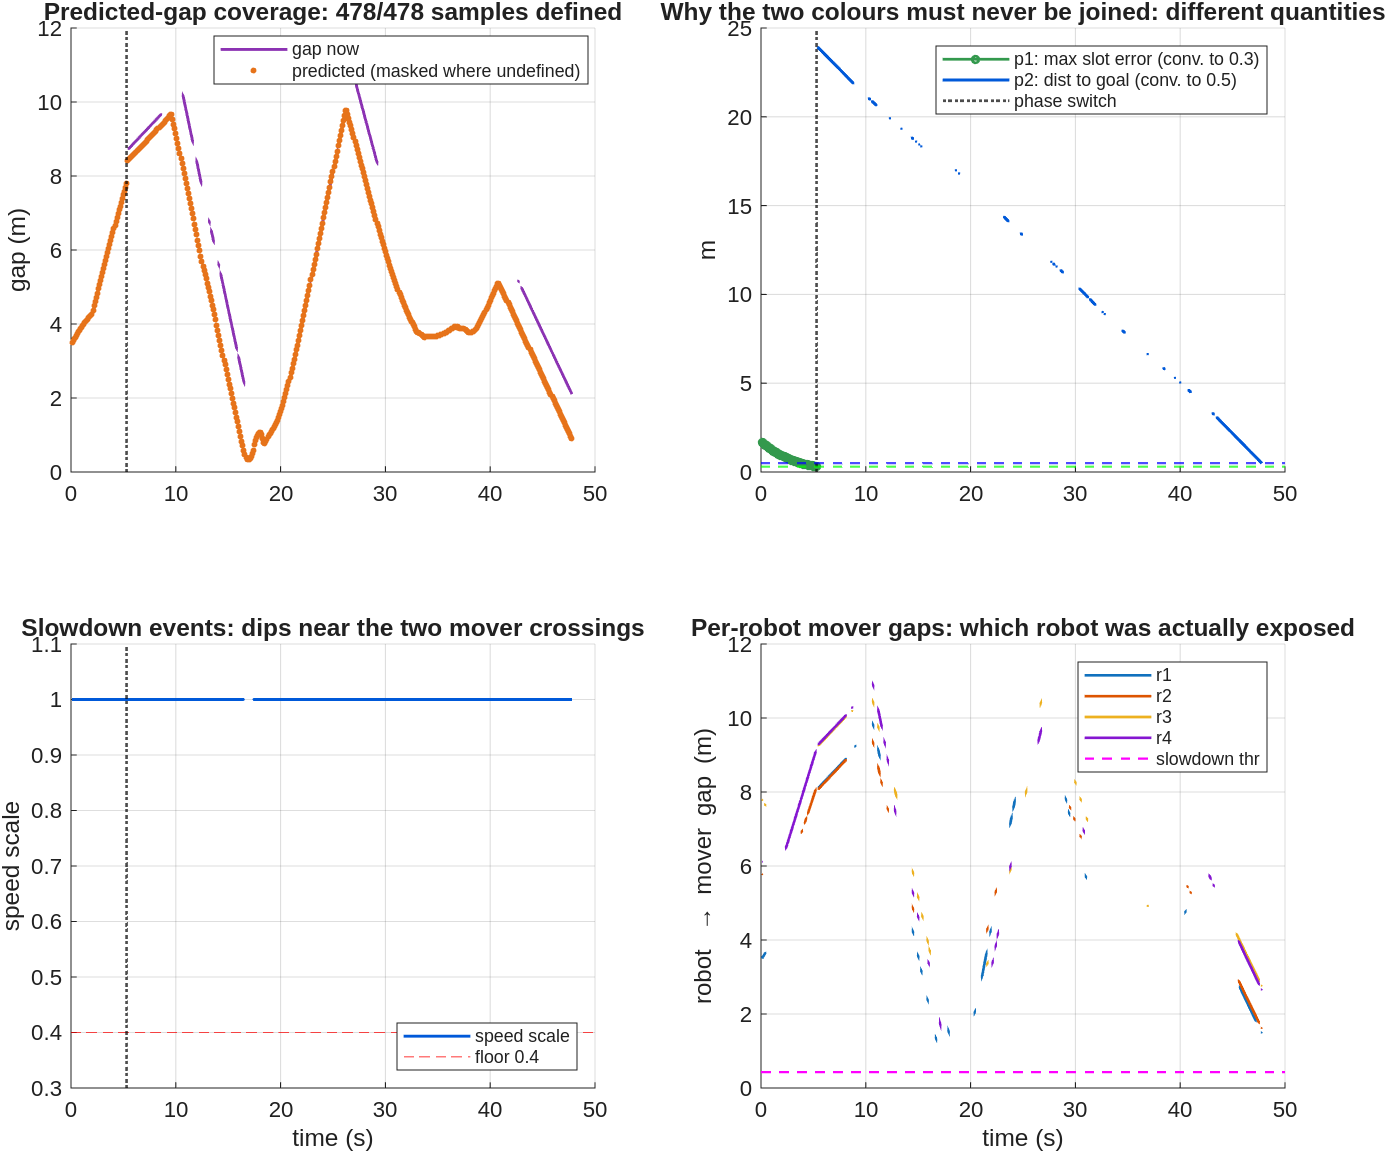
\includegraphics[width=0.94\textwidth]{figures/fig_gaps.png}
\caption{The gaps, made explicit. Top left: predicted-gap coverage against
the current gap (masked samples are simply absent). Top right: the two
semantics of the approach metric, deliberately not joined. Bottom left:
speed-scale dips at the two mover crossings. Bottom right: per-robot mover
gaps recomputed from the logged poses --- the aggregate metric hides which
robot was actually exposed.}
\label{fig:gaps}
\end{figure}

The bottom-right panel deserves a note: the logged \code{mover\_gap} is a
minimum over the whole formation. During a crossing, one robot is threatened
and the other three are fine; the aggregate says ``1.2~m'' but the per-robot
recomputation shows the exposed robot's true gap and when. Any safety argument
should be made on per-robot data.

\subsection{Trajectory map}

\begin{figure}[h]
\centering
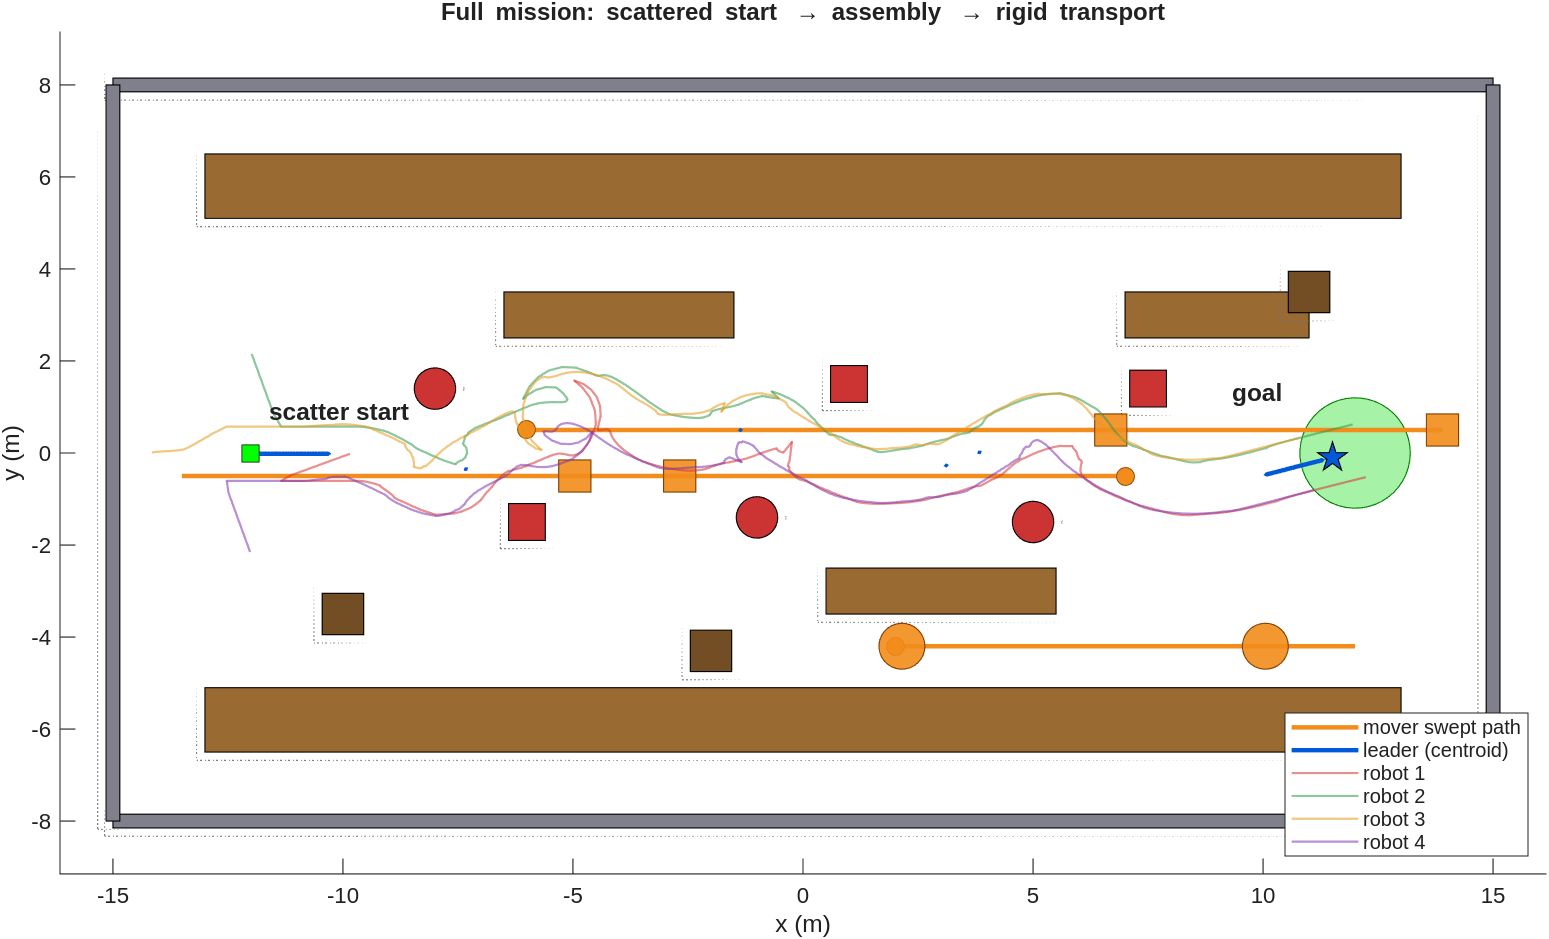
\includegraphics[width=\textwidth]{figures/fig_trajectory.png}
\caption{The whole mission. Black/dashed: warehouse. Blue line: leader
(formation-centre) trajectory. Coloured dots: the four robots during
transport. Orange: mover swept paths and poses at the two closest-approach
instants.}
\label{fig:traj}
\end{figure}

\textbf{What to look for.} (i) The coloured robot trails now cover the
\emph{whole} mission: the scatter$\to$square assembly (first $\sim$5~s of
motion, robot trails converging from the ring) and then the rigid transport.
(ii) The blue leader path bends \emph{once} around pillar4/pillar5 but is
otherwise straight: efficiency $0.93$ means avoidance was local, not global
wandering. (iii) At $x \approx -6$ and $x \approx 10.6$ the path bulges
around the orange movers --- those are the two yield events. (iv) The robot
trails stay a tight lattice through both yield events; the payload block
never clips anything.

\textbf{Failure signatures:} a leader line that doubles back (heading limit
cycle --- check the predictive scan), robot trails crossing obstacles
(collision test too weak --- is payload mode on?), or sawtooth spacing
(formation servo too stiff for the turn rate).

\subsection{Diagnostic time series}

\begin{figure}[h]
\centering
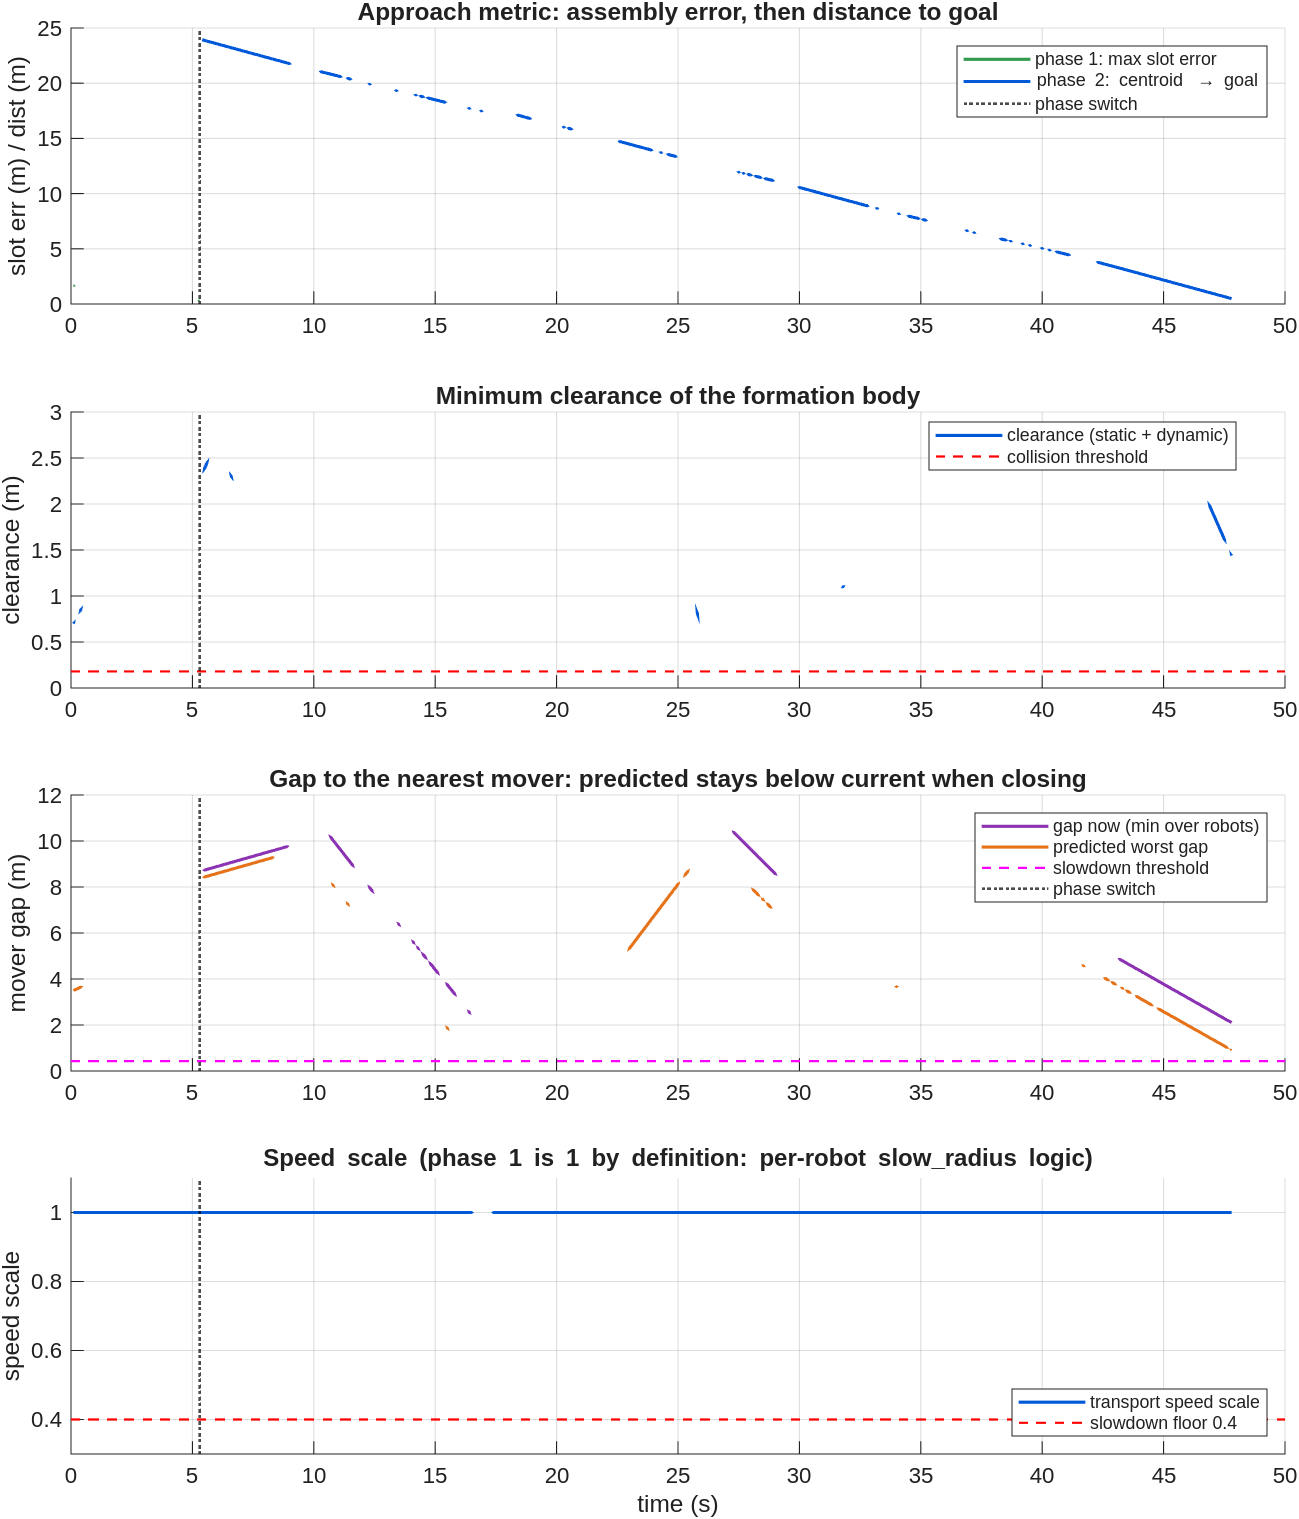
\includegraphics[width=0.86\textwidth]{figures/fig_diagnostics.png}
\caption{Top to bottom: the approach metric (green = slot error in forming,
blue = distance to goal in transport, boundary marked), formation clearance
across the whole run, mover gap now vs predicted, and the transport speed
scale. Vertical dotted lines mark the phase switch at $t = 5.4$~s.}
\label{fig:diag}
\end{figure}

\begin{itemize}[leftmargin=1.6em]
\item \textbf{Approach metric (top).} Two different quantities, two
colours, never joined. The green segment converges to the 0.3 m formation
tolerance; the blue segment then runs 23.9 m $\to$ 0.49 m. Flats in the blue
segment while clearance stays healthy mean a stall (escape logic engaged); a
rise means avoidance was worth the detour --- match it against the clearance
panel directly below.
\item \textbf{Clearance (second).} The red dashed line is the collision
threshold (robot radius). The curve dipping \emph{toward} it at the chicane
and at the mover crossings is correct --- the corridor physically pinches to
2.45 m, and the block needs 2.02 m of it. Minimum 0.51 m means the
controller used 72\% of the available margin at the worst instant and never
crossed the line.
\item \textbf{Mover gaps (third).} Purple: current gap (min over robots).
Orange: predicted worst gap over the 1 s lookahead --- it sits \emph{below}
the purple line exactly while a mover is closing, which is the whole point
of prediction. The magenta dashed line is the slowdown threshold. The two
dips are the two movers; the predicted minimum of 0.33 m is what triggered
the slowdown, while the gap that actually materialised never went below
1.22 m.
\item \textbf{Speed scale (bottom).} 1.0 everywhere except the dips near the
mover crossings (minimum 0.61). Phase 1 is constant 1 by definition ---
forming speed is governed by each robot's own slow-radius logic, not the
transport slowdown. The 0.4 floor is never reached in this run: the yield
was resolved by steering, with slowdown as assist rather than as the primary
mechanism.
\end{itemize}

\subsection{Per-robot and inter-robot graphs}

\begin{figure}[h]
\centering
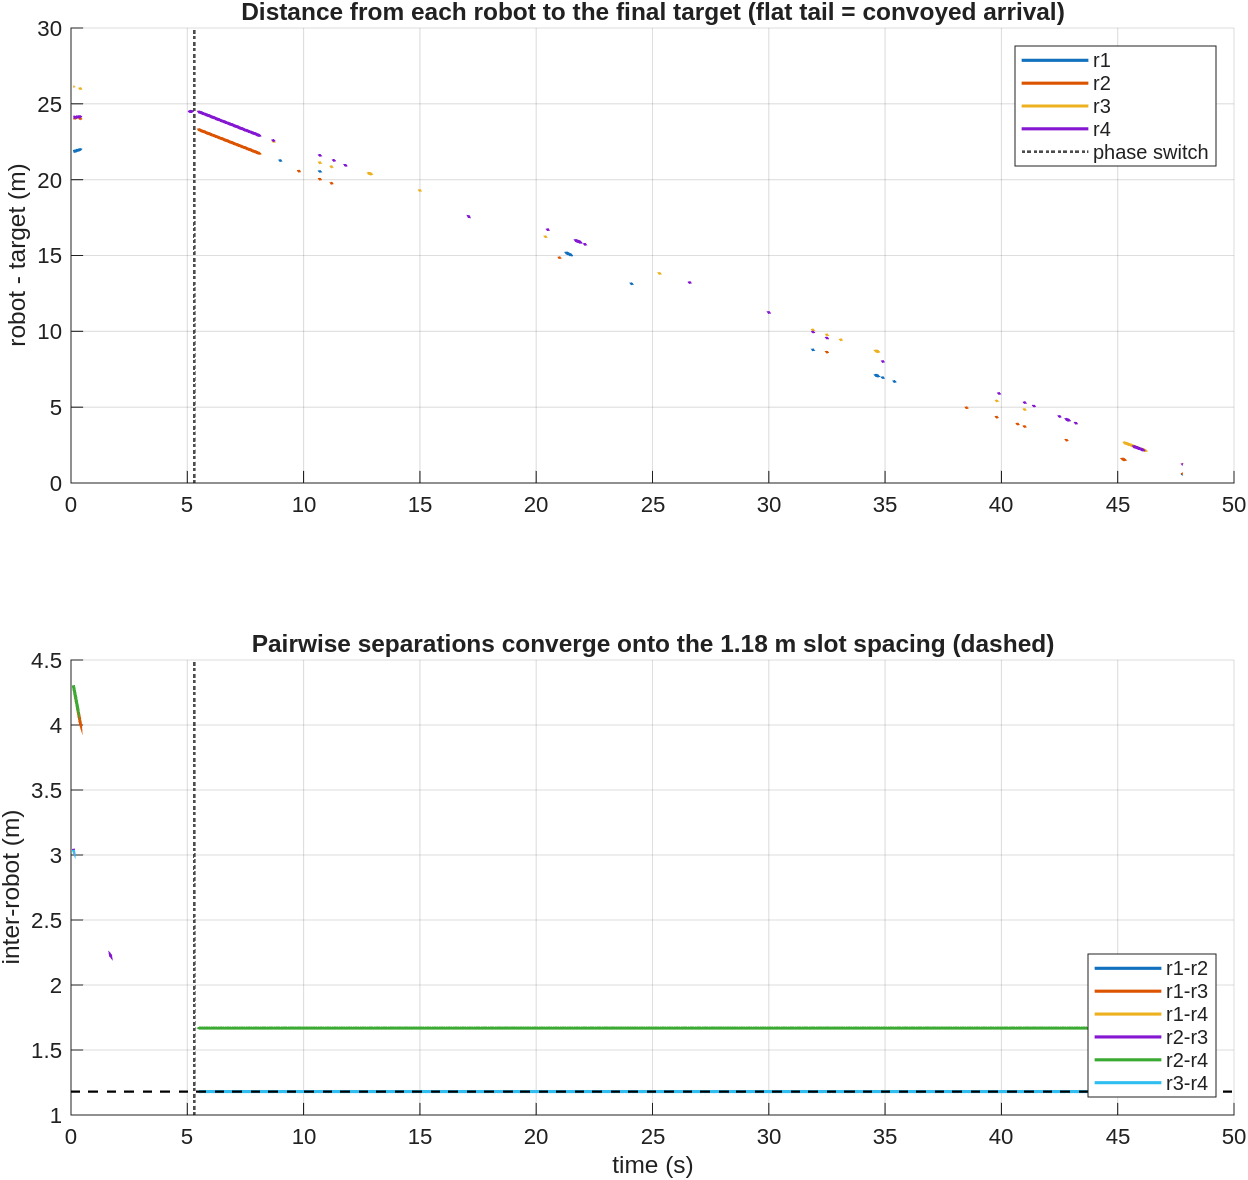
\includegraphics[width=0.86\textwidth]{figures/fig_graphs.png}
\caption{Top: distance from each robot to the final target. Bottom: pairwise
robot separations against the nominal slot spacing (dashed).}
\label{fig:graphs}
\end{figure}

\textbf{Top panel.} Four curves, one per robot. They start at different
ranges (scattered start), converge to nearly identical values within the
first seconds (assembly), then decrease together --- the signature of a rigid
body translating. The flat tail at $\approx 0.5$~m is the goal-reaching
offset: the leader stops when the \emph{centroid} is within $0.5$~m, so each
robot sits at its slot radius from the goal. Curves that cross during
transport mean the assignment permuted mid-run (should not happen; slots are
fixed after Phase~1).

\textbf{Bottom panel.} Six curves, one per robot pair. In the kinematic model
these are constant by construction --- they oscillate mildly only during
assembly and at yield events where the frame heading swings. The dashed line
is the nominal spacing $1.18$~m; all six curves sit on it after
$t \approx 5$~s. In a ROS~2 replication this panel is \emph{the} formation
quality metric: \code{formation\_rms} in \code{compare\_runs.m} is exactly
the RMS deviation of these six curves from their own mean, and any structural
difference between the stacks shows here first.

\subsection{Formation geometry}

\begin{figure}[h]
\centering
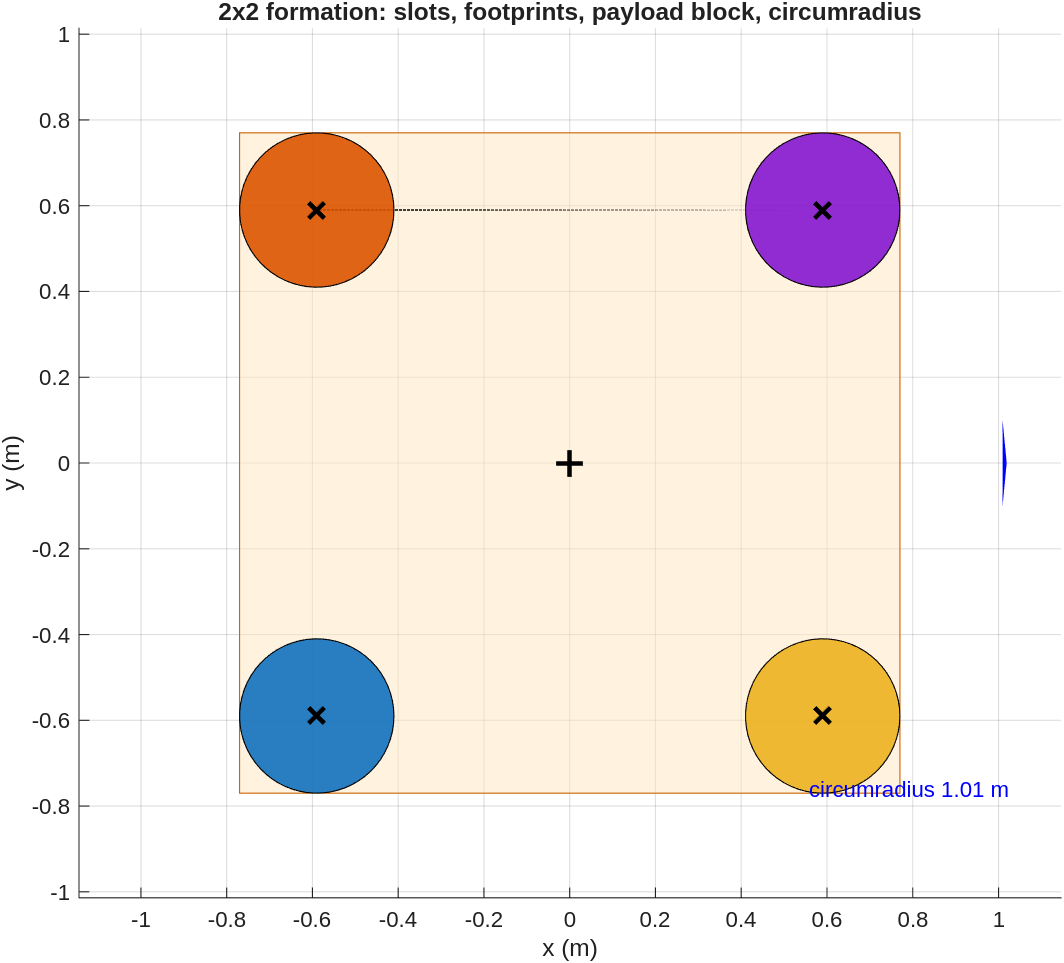
\includegraphics[width=0.62\textwidth]{figures/fig_formation.png}
\caption{The transported body. Filled circles: robot footprints at true size.
Orange: the payload block (slot square inflated by the robot radius). Blue:
the effective circumradius used for VFH enlargement and feasibility.}
\label{fig:form}
\end{figure}

This figure explains \emph{why} the spacing is what it is. The quantity that
must fit through a corridor is the circumradius
$c = 0.59\sqrt{2} + 0.18 = 1.01$~m --- not the half-width --- because the
block rotates. The bottleneck is $1.22$~m, so the margin is $0.21$~m: any
controller that drifts more than that in a turn physically cannot pass, which
is why the feasibility check runs before the simulation and why the spacing
auto-fixes to $1.18$~m rather than a round number.

\subsection{p-VFH histogram and the predictive scan}

\begin{figure}[h]
\centering
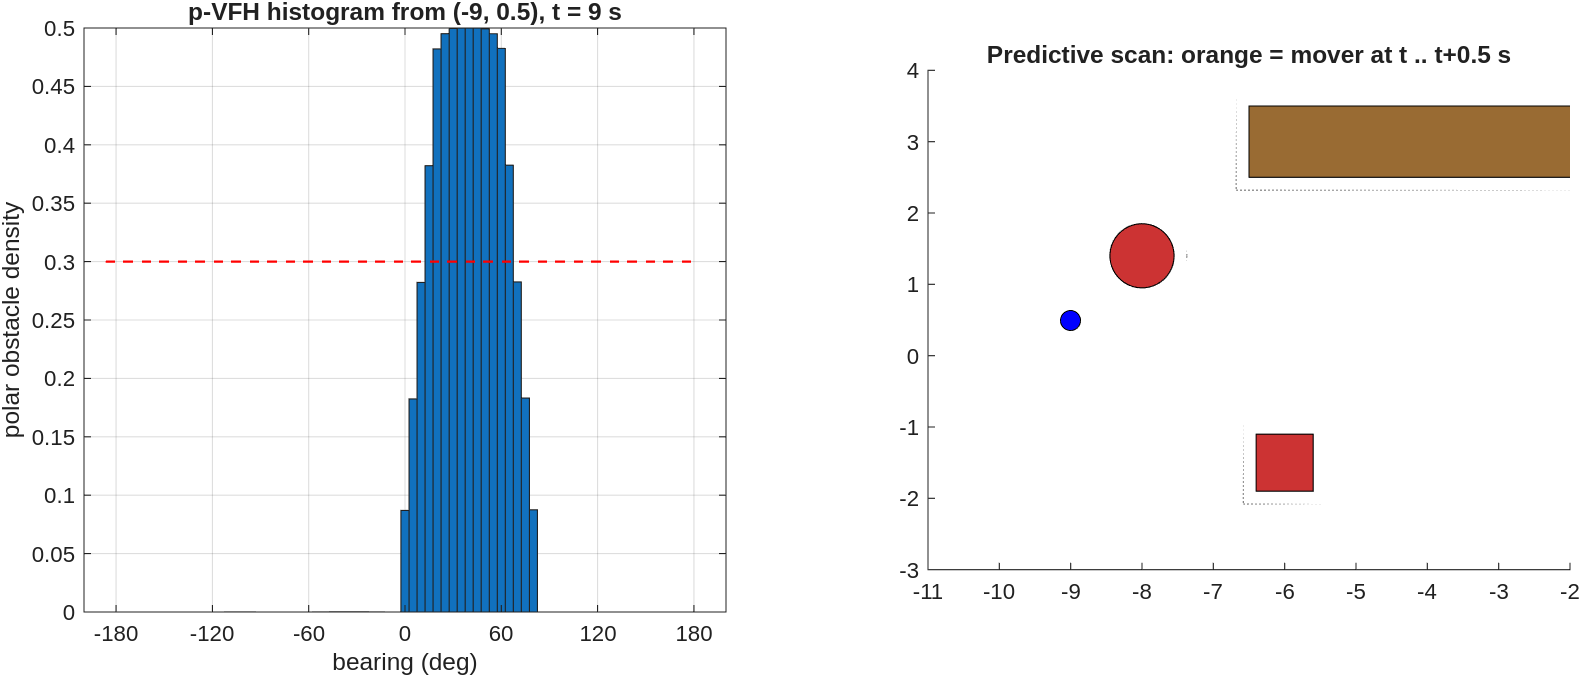
\includegraphics[width=\textwidth]{figures/fig_vfh.png}
\caption{Left: the polar obstacle density at $t = 9$~s from the formation
start position. Right: the scene --- orange rings are the mover at
$t \dots t + 0.5$~s.}
\label{fig:vfh}
\end{figure}

\textbf{Left panel.} Height is danger: sectors above the red dashed line
($\tau = 0.3$) are blocked, sectors below are candidate valleys. The broad
wall of density around $0^\circ$ is the approaching mover plus pillar1; the
walls at $\pm 90^\circ$ are the shelf faces. The controller picks the valley
closest to the goal bearing (toward $0^\circ$ here) --- so the histogram must
show a \emph{gap} between the mover and the shelves for the formation to
slip through; if the mover is centred in the aisle, no gap exists and the
yield (slowdown + detour) happens instead.

\textbf{Right panel.} The orange rings are the mover at six instants over the
prediction horizon. The nearest ring is where an instantaneous scan would see
it; the rings marching toward the robot are what \code{pvfh\_predict}
actually feeds into the histogram --- the beam keeps the \emph{nearest
blocking instance over the horizon}, which is how the controller reacts to
where the obstacle \emph{will be}.

% 09_concepts.tex -- self-contained "concept school": every idea the reader
% needs to understand Section~\ref{sec:experiments}, taught from zero with
% this project's own files as the worked examples. Video + paper references
% live in the bibliography at the end of this file.

\section{Concept school: the ideas behind the experiments}
\label{sec:concepts}

This section teaches, from zero, each idea the experimental evaluation
(Section~\ref{sec:experiments}) rests on --- reactive obstacle avoidance,
histogram steering, reasoning under sensor uncertainty, Monte Carlo
experiment grids, and the ToF-vs-LiDAR sensor trade-off. Each subsection ends
with pointers for going deeper: the paper that introduced the idea, a
textbook chapter, and at least one video lecture. The worked examples are
always this project's own files, so every concept can be seen running in
code you already have.

\begin{keybox}{Concept map --- where each idea lives in this project}
\footnotesize
\begin{tabular}{@{}p{2.9cm}p{4.6cm}p{2.6cm}p{3.1cm}@{}}
\toprule
\textbf{Concept} & \textbf{Implemented in} & \textbf{Tested by} &\textbf{Taught here} \\
\midrule
Potential fields (APF) & \code{apf\_force.m} / \code{vfh.py} reflex & E1 (local minimum) & \S\ref{sec:concept-apf} \\
Histogram (VFH) & \code{pvfh\_scan.m} + \code{steering\_dispatch.m} / \code{vfh.py} & E1--E3 baselines & \S\ref{sec:concept-vfh} \\
Sensor noise model & \code{sensor\_noise.m} / \code{vfh.py::sensor\_noise} & E2, E3, E6 & \S\ref{sec:concept-unc} \\
Probabilistic blockage & \code{pvfh\_prob.m} / \code{vfh.py::pvfh\_prob} & E2 (headline) & \S\ref{sec:concept-unc} \\
Monte Carlo grid & \code{run\_paper\_experiments.m} & E1--E14 & \S\ref{sec:concept-mc} \\
Paired seeds & same PRNG seed per run & E2, E5, E7 & \S\ref{sec:concept-mc} \\
ToF vs LiDAR & \code{sensor\_noise.m} \code{'tof'} vs \code{'lidar'} & E3, E6 & \S\ref{sec:concept-tof} \\
Formation geometry & \code{formation\_geometry.m} / \code{geometry.py} & E4, E5 & \S\ref{sec:concept-vfh} \\
\bottomrule
\end{tabular}
\end{keybox}

\subsection{Reactive obstacle avoidance I: potential fields}
\label{sec:concept-apf}

The oldest answer to ``how should a robot steer around things it can see''
is to pretend space is a landscape of hills and a valley. The goal exerts an
\emph{attractive} force, every obstacle an \emph{inflating} repulsion, and
the robot simply walks downhill on the sum:
\begin{equation}
u = k_{\mathrm{att}}\,(x_{\mathrm{goal}} - x)\; -\;
    \sum_{i} k_{\mathrm{rep}}\,\nabla \phi(d_i),
\qquad
\phi(d) \approx \Big(\tfrac{1}{d}-\tfrac{1}{d_0}\Big)^2 \ \text{for } d < d_0,
\label{eq:apf-concept}
\end{equation}
where $d_i$ is the clearance to obstacle $i$ and $d_0$ the influence radius.
Three properties matter for everything that follows:

\begin{enumerate}[leftmargin=1.9em]
\item \textbf{It is reactive.} No map, no plan --- the command is a function
of the \emph{current} scan only. That is why it costs microseconds (E1's
\code{apf} compute bar) and why it can be reflexively layered under any other
planner.
\item \textbf{It has a famous failure mode.} Two obstacle faces pushing from
opposite sides can cancel the goal attraction exactly: a \emph{local
minimum}. The robot then presses into a wall forever. This is not a bug in
one implementation; it is a theorem about eq.~\eqref{eq:apf-concept}, shown
rigorously by Koren and Borenstein \cite{koren1991}. E1's \code{apf} row
(Table~\ref{tab:e1}) is where to look for this theorem in the data: a law
that stops making progress without ever being refused by the safety gate.
\item \textbf{It fixes itself if you add a histogram.} Vector fields answer
``which way do forces point''; histograms (next subsection) answer ``which
bearings are free'', and a free-bearing search cannot be trapped the same
way.
\end{enumerate}

\paragraph{Go deeper.} Khatib introduced the real-time potential-field
method \cite{khatib1986}; Koren and Borenstein catalogued its pathologies
\cite{koren1991}. The friendliest video treatment is Chapter~10.6 of the
Northwestern \emph{Modern Robotics} course \cite{lynchvideo}, six minutes
that build eq.~\eqref{eq:apf-concept} visually; the textbook chapter behind
it is Lynch \& Park \cite{lynch2017}, \S10.6.

\subsection{Reactive obstacle avoidance II: histograms in motion (VFH)}
\label{sec:concept-vfh}

VFH replaces vector addition with \emph{voting}. Take the $n$ range beams of
the scan. Each beam $b$ measures range $d_b$ along bearing $\theta_b$. Reduce
the plane to $\alpha$ sectors of $\Delta\theta$ degrees and give each sector
an obstacle density: the classic choice, used verbatim in
\code{pvfh\_scan.m}/\code{vfh.py}, is
\begin{equation}
h_b \;=\; \Big(1-\tfrac{\min(d_b, d_{\max})}{d_{\max}}\Big)^2,
\qquad
h_k = \sum_{b \in \mathrm{sector}\,k} h_b,
\label{eq:vfh-concept}
\end{equation}
so a close return votes strongly, a far return weakly, and each sector sums
its beams' votes. Sector $k$ is \emph{blocked} when $h_k$ exceeds the
threshold \code{tau}; the robot steers into the \emph{gapped} direction
closest to the goal bearing that also respects the robot's turning radius
(a ``mask'' on candidate directions). The pipeline is exactly:
scan $\to$ per-beam kernel \eqref{eq:vfh-concept} $\to$ sector histogram
$\to$ threshold $\to$ masked gap selection $\to$ heading setpoint.

Why this cannot share APF's failure mode: the two opposing walls both vote
``blocked'' for their own sectors, but the \emph{search} over free sectors
sees the aisle between them and takes it. The failure changes character: VFH
cannot get stuck, but it \emph{can} misread --- which is where noise enters.

\paragraph{How to read any VFH plot.} A polar histogram is a wheel with one
wedge per sector; wedge height $=$ density \eqref{eq:vfh-concept}, the
horizontal line is the threshold \code{tau}, and the chosen heading is the
free wedge nearest the goal direction (drawn as an arrow). When you run
\code{Simulation8\_dynamic.m} interactively with \code{viz.enable=true}, this
wheel is the live figure to watch; the PDF flowchart in
Section~\ref{sec:pvfhflow} shows the same steps statically.

\paragraph{Go deeper.} The original paper \cite{borenstein1991} is short,
heavily illustrated and still the best read --- free PDF from Yoram Koren's
Michigan page. \emph{VFH+} \cite{ulrich1998} adds the robot-radius mask and
hysteresis our implementation inherits. The MathWorks documentation page
\cite{mwvfh} shows MATLAB's own \code{controlVFH+} object, useful to compare
parameter names. For video: a lecture on sonar sensing and VFH
\cite{vfhvideo} and the shorter ``Vector Field Histogram'' explainer
\cite{vfhvideo2}; the Wikipedia article \cite{vfhwiki} is a good 5-minute
recap with the original figures.

\subsection{Reasoning under sensor uncertainty: the probabilistic histogram}
\label{sec:concept-unc}

Deterministic VFH answers one question per beam: \emph{is the bearing
free?} --- threshold \eqref{eq:vfh-concept} against \code{tau}. With a
perfect sensor that is fine. With real sensors it fails twice:

\begin{enumerate}[leftmargin=1.9em]
\item \textbf{Missed obstacle (dangerous).} A wall at 1.6~m whose return
lands \emph{inside} the reaction envelope can still read ``free'' if the
measurement noise pushes the estimate out --- the robot drives at a wall it
just saw. This is the regime E2 probes: the high-$\sigma_0$ columns of
Table~\ref{tab:e2}, where the gate-rejection count measures exactly these
``drove at something it had just seen'' events.
\item \textbf{Flicker (wasteful).} Graded kernel values near \code{tau}
flip between free and blocked as noise arrives, so the robot brakes and
lurches --- clearance collapses even when it does not collide.
\end{enumerate}

The probabilistic layer answers a better question: \emph{given everything I
know --- range estimate, sensor variance, FoV geometry --- how likely is this
bearing to be blocked?} Three ingredients, one per answer:

\paragraph{1. A per-beam measurement distribution.} Each beam returns
$\hat d_b$ modelled as true range plus Gaussian noise, $\hat d_b \sim
\mathcal N(d_b,\, s_b^2)$, where \code{sensor\_noise.m} sets $s_b$: a flat
$\sigma_0$ for the lidar kind, and for the ToF kind a linear growth term
$s_b = \sigma_0 + k_{\mathrm{rng}}\, d_b$ with a $60^\circ$ FoV arc ---
matched to how cheap ToF arrays actually behave (\S\ref{sec:concept-tof}).

\paragraph{2. A blockage probability.} The bearing is ``blocking'' if the
\emph{true} obstacle surface lies inside the reaction envelope, i.e.\ true
range $d_b \le d_{\mathrm{block}}$. Since $\hat d_b$ is a noisy proxy for
$d_b$, that event has probability
\begin{equation}
p_b \;=\; \Pr(d_b \le d_{\mathrm{block}} \mid \hat d_b, s_b)
       \;=\; \Phi\!\Big(\frac{d_{\mathrm{block}} - \hat d_b}{s_b}\Big),
\label{eq:prise-concept}
\end{equation}
with $\Phi$ the standard normal CDF. If \eqref{eq:prise-concept} looks
familiar, it is exactly the beam model of probabilistic robotics
\cite{thrun2005} --- the same $z$-test against a range threshold, turned
into a soft membership. The floor $p_{\mathrm{unknown}} = 0.05$ applies
outside the sensor's FoV: the unobserved rear hemisphere is neither a phantom
wall nor a blind spot, it is a calibrated shrug.

\paragraph{3. Sector pooling and the expected kernel.} A sector is as
blocked as its \emph{best evidence}: independent per-beam probabilities pool
by noisy-OR,
\begin{equation}
p_{\mathrm{sector}} \;=\; 1 - \prod_{b \in k} (1 - p_b),
\label{eq:noisyor-concept}
\end{equation}
so every additional beam covering the sector genuinely adds evidence. In
the implementation this pooled probability is a \emph{diagnostic} (it is
logged and plotted, and it is the quantity a risk monitor would threshold);
the steering itself uses the kernel below, for the saturation reason given
in \S\ref{sec:pvfh}. Finally the deterministic kernel \eqref{eq:vfh-concept} is replaced by its
\emph{posterior expectation},
\begin{equation}
u_b \;=\; \sqrt{\tfrac{\sigma_h^2}{\sigma_h^2 + s_b^2}}\;
        \exp\!\Big(\!-\tfrac{d^2}{2(\sigma_h^2 + s_b^2)}\Big),
\label{eq:ukernel-concept}
\end{equation}
i.e.\ the expected value of the Gaussian danger kernel when the range is a
belief rather than a fact. Equation \eqref{eq:ukernel-concept} has two
properties that matter more than its formula:

\begin{itemize}[leftmargin=1.6em]
\item \textbf{Exact deterministic limit.} As $s_b \to 0$ the prefactor
$\to 1$ and \eqref{eq:ukernel-concept} $\to$ \eqref{eq:vfh-concept}: with a
perfect sensor P-VFH \emph{is} the deterministic histogram
(Proposition~1). The paired-difference plot of
Section~\ref{sec:paired} is where this shows up as data: the P-VFH~$-$~pVFH
difference should shrink toward zero at the low-noise end.
\item \textbf{A reaction envelope that widens with noise, never
saturation.} The range at which a return starts to block grows with $s_b$
(Proposition~2, Fig.~\ref{fig:theory}) --- uncertainty makes
the robot react \emph{earlier}. Note the precise statement: the kernel
\emph{value} rises with noise only for returns beyond
$\sqrt{\sigma_h^2 + s_b^2}$; very near returns read slightly lower but stay
far above the threshold. (An earlier version of this report claimed the
kernel inflates at every range; that was wrong.)
\end{itemize}

The one-sentence summary: \textbf{VFH thresholds a histogram of measurements;
P-VFH thresholds a histogram of beliefs.}

\paragraph{Go deeper.} Thrun, Burgard \& Fox, \emph{Probabilistic Robotics}
\cite{thrun2005}: Chapter~2 (recursive state estimation) and the beam
models of Chapter~6 are the mathematical home of \eqref{eq:prise-concept}.
Cyrill Stachniss's video lectures are the standard free companion: the Bayes
filter lecture \cite{stachnissbayes} builds the inference behind ``probability
of a hypothesis given a noisy measurement'', and his 5-minute occupancy-grid
explainer \cite{stachnissgrid} shows the identical free/blocked/unknown
triage P-VFH applies per sector.

\subsection{Monte Carlo experiments: factors, grids, cells, seeds}
\label{sec:concept-mc}

A robot run is stochastic --- noise realisations differ run to run --- so one
run proves nothing. The fix is to run the mission many times under a
controlled experimental grid and report statistics. Section~\ref{sec:gridconcept}
gives the operational vocabulary; here is the reasoning behind it.

\begin{keybox}{The five words, in one breath}
A \textbf{factor} is what you vary on purpose; its values are
\textbf{levels}; the \textbf{grid} is every combination of levels; one
combination is a \textbf{cell}; one full mission executed in a cell under
one \textbf{seed} (a pinned random number generator) is a \textbf{run}.
Repeat runs with different seeds and report means/rates/spreads:
that repetition is the \textbf{Monte Carlo} method.
\end{keybox}

\paragraph{Why the seed is the most important knob.} Seeding the PRNG
(``random'' numbers drawn from a reproducible generator) makes a stochastic
experiment \emph{replayable}. Every run is seeded explicitly (MATLAB \code{rng(seed)}; Octave
\code{randn('seed',...)}; the Python port \code{np.random.default\_rng(seed)}). Consequences you can rely on:
re-running a cell reproduces its CSV byte-for-byte (a regression test in
itself), and --- the design trick --- \emph{two algorithms sharing a seed
see the identical noise realisation}. Their per-seed difference then
contains no noise variance at all, only the steering-law difference: a
paired comparison, the experimental analogue of a paired t-test. That is
why Section~\ref{sec:paired} can resolve small clearance differences with
just five seeds.

\paragraph{Reading results honestly.} Three habits:
(i) report \emph{success rate and collisions beside every mean} --- a cell
that reaches 60\% of the time with a beautiful mean clearance is a failing
cell; (ii) compare cells that differ \emph{only} in the factor your question
is about (``ceteris paribus'' --- all E1 algorithms consume the same scan
and gains); (iii) long-format CSVs (one row per run) are the safe storage,
because any summary is then a trivial \code{GROUP BY}.

\paragraph{Go deeper.} Art Owen's in-progress Monte Carlo book
\cite{owen2019} is free online; Chapter~1 motivates exactly our setup
(estimate an expectation by sampling, report the error) and Chapter~9 covers
variance reduction --- of which paired seeds are the simplest instance. For
a 10-minute video, Steve Brunton's lecture on Monte Carlo sampling
\cite{bruntonmc} shows the estimator and its error bars; the same channel's
``Crude Monte Carlo'' demonstration \cite{bruntoncrude} is a worked example
of seeding and error shrinkage with sample size.

\subsection{ToF vs LiDAR: what the sensor choice does to a planner}
\label{sec:concept-tof}

E3 sweeps beam counts but the deeper hardware question is \emph{which
sensor technology}, and E6 (\S\ref{sec:e6}) answers it directly with a
matched design. The physics of the two contenders:

\begin{itemize}[leftmargin=1.6em]
\item \textbf{LiDAR} (e.g.\ a rotating 288-beam unit): time-of-flight laser
ranging over a wide FoV at high angular resolution. Accurate and dense
--- that is the ``$288$ beams, $\sigma_0 = 0.02$'' reference row --- but
mechanically complex and comparatively expensive.
\item \textbf{ToF arrays} (e.g.\ ST VL53-series): solid-state flash LiDAR
on a chip --- a fixed grid of zones (8--64) over a narrow FoV, no moving
parts, a few dollars, but coarse angular resolution, narrow field, and
range error that \emph{grows with distance} (multipath and return-strength
effects). That growth is what the \code{'tof'} noise model encodes:
$s_b = \sigma_0 + k_{\mathrm{rng}}\, d_b$ inside a $60^\circ$ arc that is
fixed to the \emph{body} (the fan turns with the payload heading).
\end{itemize}

Two experimental-design warnings before reading E6's tables. First, the
comparison must be \emph{matched}: same world, same seeds, same algorithm,
same $\sigma_0$ --- only the sensor kind differs --- otherwise the effect of
``sensor'' is confounded with everything else. (This is
\S\ref{sec:gridconcept}'s rule~1 applied a second time.) Second, distinguish
the two axes of ``less sensor'': \emph{resolution} (beam count, E3) and
\emph{noise structure} (homoscedastic vs range-growing, E6). A sensor can
lose beams without losing reliability --- the $p_{\mathrm{unknown}}$
floor keeps unobserved bearings from being read as confidently free --- but
range-growing noise is a different attack: it blurs \emph{far} obstacles,
precisely where early warning lives. When you read E6's numbers, keep the
two effects a sensor change mixes apart: \emph{angular coverage} (FoV, beam
count) and \emph{per-return noise growth} ($s_b$). They can pull in opposite
directions: a narrow fan sees fewer side obstacles to react to, but it is
also blind to anything approaching from the side or rear --- which is where
the mover-contact column of Table~\ref{tab:e6} becomes the one to watch.

\paragraph{Go deeper.} ST's VL53L5CX product page \cite{stvl53} documents a
typical 8$\times$8 ToF array (FoV, zones, range-accuracy curve --- compare
with \code{sensor\_noise.m}'s parameters); SEEED's TF-Luna wiki \cite{tfluna}
is the cheapest reverse example (single-beam ToF, serial output). For the
planner's side of the trade, re-read \S\ref{sec:concept-unc} with ``which
$s_b$ curve am I feeding it?'' in mind.

\subsection{Self-check: five questions you can now answer}

\begin{enumerate}[leftmargin=1.9em]
\item Why can \code{apf} fail \emph{silently} (no gate rejections, no goal)
while a noisy deterministic histogram fails \emph{loudly} (many rejections)? \emph{(Local minimum vs
thresholded noise: \S\ref{sec:concept-apf}, \S\ref{sec:concept-unc}.)}
\item Which equation guarantees P-VFH reduces to VFH for a perfect sensor,
and which figure shows that as data? \emph{(Eq.~\eqref{eq:ukernel-concept};
Fig.~\ref{fig:paired} at low $\sigma_0$.)}
\item Your ToF array drops from 16 to 8 beams. What keeps the bearings no
beam covers from being read as confidently free, and which experiment
measures the cost? \emph{(The $p_{\mathrm{unknown}}$ floor; E3 and E6 ---
watch the mover-contact column.)}
\item Two algorithms share seed 3. Their min-clearance difference on that
seed is 0.4~m. Can noise explain it? \emph{(No --- paired design,
\S\ref{sec:concept-mc}.)}
\item Why is a ``flat goal rate, sagging clearance'' pattern a warning light
rather than good news? \emph{(The margin is what absorbs the next surprise;
\S\ref{sec:e3} how-to-read.)}
\end{enumerate}

\paragraph{References.} The complete reference list for the whole report
(videos included) is printed once at the end of the document.

\section{Experimental evaluation}
\label{sec:experiments}

The claims of Section~\ref{sec:pvfh} are tested with a Monte Carlo study of
fourteen experiments (E1--E14). Every run is the full two-phase mission (forming
$+$ rigid transport); the driver is \code{run\_paper\_experiments.m}
(\S\ref{sec:howto} has every command).

% AUTO-GENERATED by matlab/make_paper_figures.py -- do not edit
\begin{keybox}{Provenance of every number and figure in this chapter}
Source table: \code{matlab/logs/paper/results\_all.csv} (modified 2026-10-02 22:49); stack: matlab; 2730 runs: E1 (80), E10 (160), E11 (200), E12 (160), E13 (480), E14 (50), E2 (400), E3 (80), E5 (320), E6 (240), E7 (320), E8 (200), E9 (40). Safety-gate soundness check: 0 static-contact steps in total (must be 0). Every table and figure below is regenerated from this one file by \code{make\_paper\_figures.py}; none is typed by hand.
\end{keybox}


\paragraph{How this chapter is written.} Every table and figure below is
generated by one script from one results file, so a table and the figure
next to it cannot disagree. The prose explains the design, the metrics and
how to read each result; it deliberately does \emph{not} quote result
values, because a number typed into a paragraph is exactly how the previous
version of this chapter came to contradict its own figures
(\S\ref{sec:audit}). Read the numbers off the tables. The one exception is
\S\ref{sec:findings}, which states the findings of one specific grid and
says which.

\paragraph{What ``experimental validation'' means here (and what it does
not).} \label{sec:simvalidation}
Every experiment in this chapter is an \emph{in-simulation, controlled
experiment} --- Monte Carlo runs over synthetic worlds
(\S\ref{sec:model-kinematics}), synthetic sensors and synthetic noise ---
not a physical-robot trial. This is the right instrument for the questions
asked here (which steering law degrades how, under which noise, at what
compute cost), because simulation is the only setting where the noise, the
world and the seeds can be held fixed and varied one factor at a time. What
it does not establish: actuation dynamics (wheel slip, torque limits,
latency), sensing artefacts beyond the noise model (occlusion by the
payload itself, dropouts, multi-path ghosts), localisation error, and
communication faults. Two idealisations deserve to be named because they
favour every algorithm equally but are still idealisations: the scan is
taken from the formation centroid, and the safety gate
(\S\ref{sec:gate}) knows the true geometry. A physical-robot campaign and a
second, independent implementation remain future work
(\S\ref{sec:roadmap}). The conclusions to trust most are therefore the
\emph{relative, algorithm-level} ones; absolute values are properties of
these worlds and this parameter set.

\subsection{Audit of October 2026: what was wrong and what changed}
\label{sec:audit}

The previous version of this chapter reported tables from one
implementation (Octave) and drew several figures from another (a Python
port), and its text explained the disagreements between the two as findings.
An audit of the MATLAB reference against its own per-step logs found that
most of those ``findings'' were defects. They are listed here because they
change what the earlier numbers meant.

\begin{enumerate}[leftmargin=1.9em]
\item \textbf{Unchecked rotation (the source of every reported collision).}
The transport loop committed the new heading before, and regardless of, the
collision check; only the translation was gated. A blocked body therefore
kept rotating in place \emph{into} the obstacle. In the pre-fix logs every
collision step examined has zero translation and non-zero yaw change. The
``collision steps'' column of the old E1/E2/E5/E6 tables measured this
artefact. Fixed by the atomic pose commit of \S\ref{sec:gate}.
\item \textbf{\code{'pvfh'} was noise-free.} It raycast a clean
full-circle lidar and never called the sensor model, so the ``verified
reference'' was an oracle: its trajectories were bit-identical across seeds.
The statement that all variants consume the same noisy scan was false for
it. Fixed: it now senses through the shared front end.
\item \textbf{\code{'vfh'} on a ToF array used the wrong bearings.} It
rebuilt its beam angles as a full circle whatever the sensor, smearing a
$60^\circ$ fan over $360^\circ$. The old text attributed the resulting
failures to the ToF noise model. Fixed: bearings come from the scan.
\item \textbf{The reflex over-weighted ToF returns six-fold.} The APF
reflex integrated over bearing with a beam width of $2\pi/n$ even for a
$60^\circ$ fan. Fixed: the scan reports its beam width.
\item \textbf{\code{'vfh'} had a prediction horizon it was documented not
to have}, and an ``instantaneous'' scan (horizon $0$) could not see movers
at all. Fixed on both counts.
\item \textbf{The ToF fan was fixed to world $+x$}, not to the body. Fixed:
body frame by default.
\item \textbf{The noisy-OR risk layer never influenced steering}, although
the text credited it with the sparse-sensor results; and the claimed
property $\partial u_b/\partial s_b > 0$ at every range is false. The text
is corrected and the true statement is proved (Proposition~2,
\S\ref{sec:pvfh}).
\item \textbf{The ToF noise model was written two ways}: linear,
$s_b = \sigma_0 + k_{\mathrm{rng}} d_b$, in the code and in
\S\ref{sec:sensornoise}; in quadrature in this chapter. The code's linear
form is the model; the text now agrees.
\item \textbf{The mean compute time mixed three things}: phase-1 values
summed over the robots, phase-2 values, and zeros from escape steps. It is
now the phase-2 steering cost only.
\item \textbf{Figure defects.} The time-series figure coloured two
algorithms opposite to every other figure and carried hand-placed
annotations at fixed times; the trajectory figure had an empty panel; the
formation sketch quoted circumradii in units of $s$ while the table beside
it quoted metres at a different spacing; captions described traces the
figure did not show. All figures are now generated with one colour and one
order per algorithm, on the world map, with annotations taken from the logs.
\item \textbf{The P-VFH kernel was evaluated with the wrong division.}
\code{pvfh\_prob.m} computed $\exp(-d^2 / 2(\sigma_h^2 + s_b^2))$ with
MATLAB's matrix division instead of the element-wise one. For two row
vectors that returns \emph{one} least-squares scalar, so every beam
received the same kernel value and the histogram was the same in every
direction. Every result attributed to P-VFH before this was found ---
including the first corrected grid --- was produced by a law that could
not tell a blocked bearing from a free one and steered by goal attraction
and reflex only. Its apparent insensitivity to range noise was this
defect. (The Python port had the formula right, which is one more reason
the two implementations disagreed.) Fixed; with the kernel working, the
single-scan P-VFH behaves like the deterministic law, and the noise
robustness now comes from the range filter of \S\ref{sec:rfilter}.
\item \textbf{Two mover-handling crashes.} The distance routine referenced
an undefined variable when there were no movers, and the routine that
merges movers into the map deleted a real static obstacle whenever all
movers were of one shape. Both fixed.
\item \textbf{The anti-deadlock layer existed only in the Python port} and
was disabled there for \code{'apf'}. It is now part of the MATLAB reference
and applies to every law (\S\ref{sec:gate}); E9 reports it as an ablation.
\end{enumerate}

Consequences for interpretation: because the gate now covers rotation,
static contact cannot occur and is reported only as a soundness check; the
safety comparison between laws is carried by \textbf{gate rejections},
\textbf{mover contacts} and the \textbf{minimum surface gap}. The earlier
headline (``the deterministic histogram collides and collapses, P-VFH does
not'') was established on the defective loop and must be re-established on
the corrected one before it is claimed. The Python port has been brought
in line with these fixes since the audit; its results are reported as an
independent replication in Section~\ref{sec:replication}. One remaining
item of the audit list --- the reference gate's corner-order defect
(section~\ref{sec:audit-gate} below and section~5.3 of the
documentation) --- is not a port item: it is a flaw in the MATLAB reference
itself, fixed by changing two corner orders in \code{formation\_clearance\_dyn.m},
and the corrected comparison is reported in Sections \ref{sec:cross} and
\ref{sec:replication}.

\subsection{The reference gate defect and what it changes}
\label{sec:audit-gate}

The MATLAB test (\S\ref{sec:gate} of the prior report) listed a box's
corners in the order $(+,+), (+,-), (-,+), (-,-)$ and took the ``edges''
between consecutive entries. That order is not a walk around the box: the
four ``edges'' are the two vertical sides and the two \emph{diagonals}. One
of the box's two edge normals is therefore never tested, and some poses
that are in fact collision-free are reported as overlapping. The defect is
conservative: it never misses a real overlap (verified against a
brute-force distance computation), it only refuses some safe poses. It
inflates the headline rejection count at low noise (3--7 spurious
rejections per run for the histogram laws in E1/E2 at sigma0 = 0.02 m) but
changes no ranking between laws and no static-contact count.

The corrected gate is the default on the Python stack and is reported
alongside the reference gate in the replication (Table~\ref{tab:cross_exact}).
On the MATLAB stack the fix is two corner orders in
\code{formation\_clearance\_dyn.m}; the grid should be re-run there so the
reference tables stop carrying a known artefact.

\subsection{Experiment design}

\begin{table}[H]
\centering
\footnotesize
\begin{tabular}{@{}l>{\raggedright\arraybackslash}p{6.6cm}>{\raggedright\arraybackslash}p{5.6cm}@{}}
\toprule
 & \textbf{Factors and levels} & \textbf{Question} \\\midrule
E1 & law: \code{apf}, \code{vfh}, \code{fgm}, \code{dwa}, \code{mpc},
\code{pvfh}, \code{pvfh\_filt}, \code{pvfh\_prob} \newline (lidar-288, $\sigma_0 = 0.02$) &
Which steering laws complete the mission, at what margin and cost? \\\\\
E2 & law: \code{vfh}, \code{pvfh}, \code{pvfh\_filt}, \code{pvfh\_prob}; \newline $\sigma_0 \in
\{0.02, 0.05, 0.10, 0.20, 0.40\}$~m; double seeds &
Does the probabilistic occupancy degrade more gracefully than the
deterministic one as range noise grows? \\\\\
E3 & law: \code{pvfh}, \code{pvfh\_prob}; beams $\in \{288, 64, 16, 8\}$
($\sigma_0 = 0.10$; below 288 a $60^\circ$ ToF fan) &
How much of the sensor can be removed? \\\\\
E4 & shape: square, diamond, triangle, line at $s=0.60$~m, \code{pvfh\_prob} &
Which payload layouts does the corridor network admit? (The P-VFH rows of
E5, not separate runs.) \\\\\
E5 & shape $\times$ law ($4\times8$) at $s=0.60$~m &
Does the \emph{shape} break the \emph{law}? \\\\\
E6 & sensor: lidar-288, tof-16, tof-8; $\sigma_0 \in \{0.02, 0.10\}$;
law: \code{vfh}, \code{pvfh}, \code{pvfh\_prob} &
With everything else fixed, what does the sensor alone change? \\\\\
E7 & world: plaza, maze; eight laws; $\sigma_0 \in \{0.02, 0.20\}$ &
Do the conclusions survive outside the warehouse? \\\\\
E8 & mover speed $\times \{0.5, 1, 1.5, 2\}$; \code{vfh}, \code{dwa},
\code{mpc}, \code{pvfh}, \code{pvfh\_prob} &
How does each law cope as traffic speeds up? \\\\\
E9 & anti-deadlock layer off; line shape; \code{vfh}, \code{pvfh},
\code{pvfh\_prob} &
What does the mission-level layer contribute? \\\\\
E10 & pose-estimate noise $\sigma_p \in \{0, 0.05, 0.15, 0.30\}$~m (yaw
noise $20^\circ$ per metre of $\sigma_p$); \code{dwa}, \code{mpc},
\code{pvfh}, \code{pvfh\_prob} &
How much localisation error does each law tolerate? \\\\\
E11 & number of movers $\in \{0, 1, 3, 6\}$; \code{vfh}, \code{dwa},
\code{mpc}, \code{pvfh}, \code{pvfh\_prob} &
How does each law scale with traffic density? \\\\\
E12 & probability a steering update is lost $\in \{0, 0.1, 0.3, 0.5\}$;
\code{dwa}, \code{mpc}, \code{pvfh}, \code{pvfh\_prob} &
How sensitive is each law to dropped commands? \\\\\
E13 & ten randomly generated layouts; eight laws;
$\sigma_0 \in \{0.02, 0.20\}$; 3 noise seeds per layout &
Do the conclusions hold on layouts nobody designed by hand? \\\\\
E14 & load-carrying motion limits on; \code{vfh}, \code{dwa}, \code{mpc},
\code{pvfh}, \code{pvfh\_prob} &
What does physically feasible turning cost? \\
\bottomrule
\end{tabular}
\caption{The experiments. Default: 10 seeds per cell (20 in E2). Identical
configurations that appear in two experiments (for example the E6 lidar
cells and the matching E2 cells) are simulated once and reported under
both labels.}
\label{tab:expdesign}
\end{table}

\paragraph{What exactly is random.}
\label{sec:mc-what-random}
The seed fixes the sensor-noise stream; the obstacle layout and the movers'
schedule are fixed per world. No algorithm draws random numbers of its own.
Two laws sharing a seed start from the same noise stream and receive the
same realisation for as long as their trajectories coincide; once they
diverge they are at different places asking for different scans, so the
pairing is a \emph{common-random-numbers} design that reduces variance, not
a guarantee of identical inputs. (The earlier text claimed identical noise
``for every scan''; that holds only up to the first divergence.)

\paragraph{Metrics.} Per run: goal reached (within $0.5$~m, before the
$300$~s timeout); \emph{gate rejections}; \emph{mover-contact steps};
static-contact steps (soundness check, must be zero); minimum
\emph{surface gap} (logged clearance minus the robot radius, so contact is
gap $\le 0$); path efficiency (straight-line distance over driven distance
--- on the maze the route is not straight, so compare efficiency only
within a world); mission time; steering compute per step.

\paragraph{Statistics.} Reach rates carry Wilson 95\% intervals; means carry
percentile-bootstrap 95\% intervals over seeds. Comparisons between two laws
are paired by seed: a Wilcoxon signed-rank test on the per-seed differences
and an exact McNemar test on the discordant reach outcomes
(Table~\ref{tab:stats}). With 10--20 seeds per cell these tests can confirm
large effects and cannot confirm small ones; an interval that spans zero is
reported as such rather than read as a difference.

\subsection{What a ``parameter grid'' is, and how to read one}
\label{sec:gridconcept}

\begin{keybox}{The vocabulary, once and for all}
A \textbf{factor} is an input varied on purpose (law, noise level, beam
count, shape, world). Its values are its \textbf{levels}. The \textbf{grid}
is the Cartesian product of the levels: every combination appears once per
\textbf{seed}. A \textbf{cell} is one combination; a \textbf{run} is one
mission in one cell with one seed. \textbf{Monte Carlo} means repeating
runs over seeds and reporting statistics instead of a single outcome.
\end{keybox}

Three rules make a grid trustworthy. \textbf{One factor per question}:
compare cells that differ only in the factor the question is about.
\textbf{Paired seeds}: comparing two laws within a seed removes part of the
run-to-run variance (\S\ref{sec:paired}). \textbf{Never average away
failures}: a cell that reaches the goal 60\% of the time with a good mean
gap is a failing cell, which is why the reach count is printed beside every
mean.

\subsection{E1 --- the steering laws}
\label{sec:e1}

% AUTO-GENERATED by matlab/make_paper_figures.py -- do not edit
\begin{table}[H]
\centering\scriptsize
\begin{tabular}{@{}lrrrrrrr@{}}
\toprule
\textbf{Law} & \textbf{Reach} [95\% CI, \%] & \textbf{Gate rej.} & \textbf{Static} & \textbf{Mover} & \textbf{Min gap (m)} [95\% CI] & \textbf{Eff.} & \textbf{Time (s)} \\
\midrule
APF & 10/10 [72,100] & 66.5 & 0 & 31.2 & -0.37 [-0.51,-0.24] & 0.37 & 119 \\
VFH & 10/10 [72,100] & 1.6 & 0 & 0.0 & 0.17 [0.14,0.20] & 0.90 & 49 \\
FGM & 10/10 [72,100] & 61.7 & 0 & 24.9 & -0.14 [-0.29,0.00] & 0.66 & 72 \\
DWA & 10/10 [72,100] & 0.0 & 0 & 0.0 & 0.13 [0.12,0.14] & 0.91 & 50 \\
MPC & 10/10 [72,100] & 0.0 & 0 & 0.0 & 0.23 [0.22,0.24] & 0.97 & 46 \\
pVFH & 10/10 [72,100] & 4.5 & 0 & 0.0 & 0.19 [0.16,0.23] & 0.89 & 50 \\
pVFH+F & 10/10 [72,100] & 4.3 & 0 & 0.0 & 0.21 [0.17,0.24] & 0.89 & 50 \\
P-VFH & 10/10 [72,100] & 5.8 & 0 & 0.0 & 0.21 [0.17,0.24] & 0.89 & 50 \\
\bottomrule
\end{tabular}
\caption{E1. Reach: runs reaching the goal, Wilson interval. Gate rej.: mean steps per run in which the safety gate refused the commanded motion. Static: total static-contact steps over the cell (must be 0). Mover: mean steps per run in contact with a mover. Min gap: mean over runs of the per-run minimum surface gap, bootstrap interval. $\dagger$ = legacy pre-fix table, where this column is the old collision-step count.}
\label{tab:e1}
\end{table}


\begin{figure}[H]
\centering
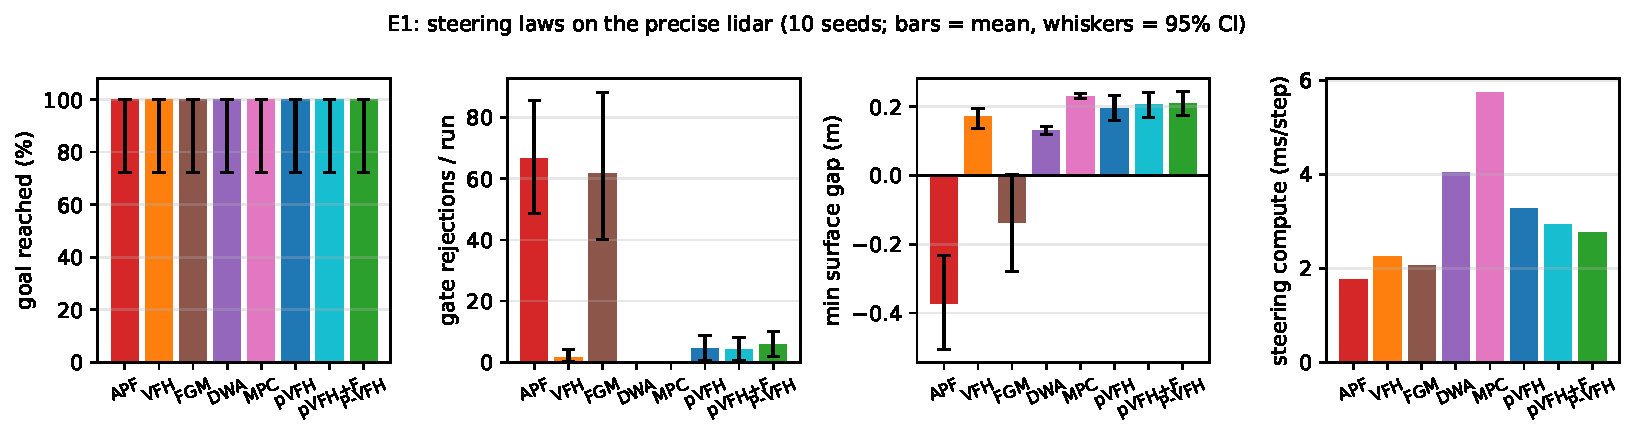
\includegraphics[width=\textwidth]{figures/algo_bars.pdf}
\caption{E1 summary per law: reach rate, gate rejections, minimum surface
gap, steering compute.}
\label{fig:e1bars}
\end{figure}

\begin{figure}[H]
\centering
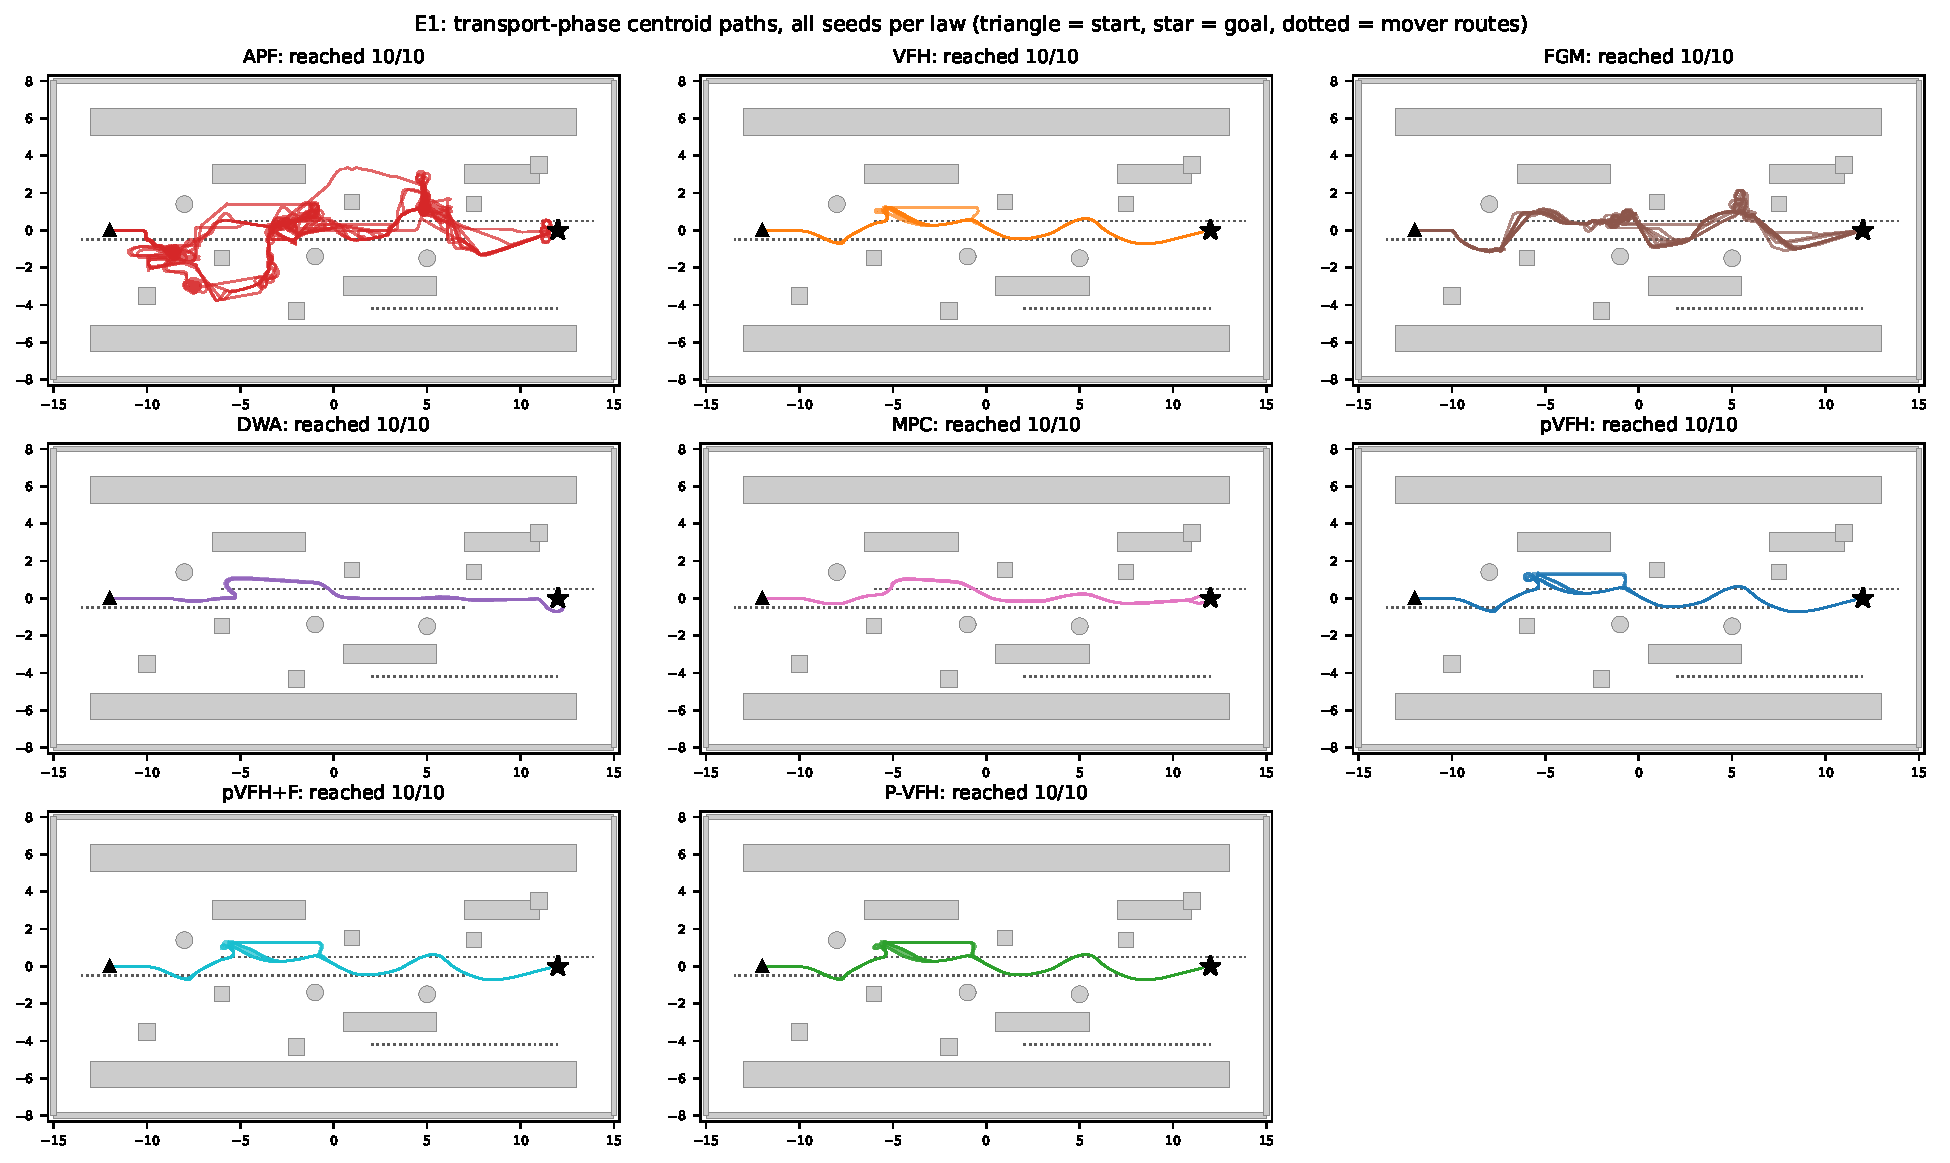
\includegraphics[width=\textwidth]{figures/trajectory_overlays.pdf}
\caption{E1 transport-phase centroid paths on the warehouse map, one panel
per law, every seed overlaid.}
\label{fig:overlays}
\end{figure}

\paragraph{How to read E1.} Start with reach: a law that does not arrive
has no meaningful efficiency. Then read the two safety columns together. A
law with few gate rejections and a healthy gap steered clear by itself; a
law with many rejections arrived only because the supervisor kept refusing
its commands. A law that fails to arrive with \emph{no} rejections is in a
local minimum (the classical APF failure, \S\ref{sec:concept-apf}): it
stopped making progress without ever asking for an unsafe move. In
Fig.~\ref{fig:overlays}, tight bundles mean the law's decisions are
insensitive to the noise realisation; fanned bundles mean they are not.
The compute panel matters only relative to the 100~ms control period.

\subsection{E2 --- noise ablation}
\label{sec:e2}

The central experiment. As $\sigma_0$ grows, a deterministic histogram
thresholds a kernel of the \emph{measured} range, so one outlier can open
or seal a corridor. P-VFH answers with two things: the range filter of
\S\ref{sec:rfilter}, whose gain is set by the sensor model, and the
expected kernel. The ladder \code{pvfh} $\to$ \code{pvfh\_filt} $\to$
\code{pvfh\_prob} separates them. The predictions to test: the filter step
should cut gate rejections and mission time at high $\sigma_0$ and change
nothing at low $\sigma_0$; the kernel step is the open question.

\begin{figure}[H]
\centering
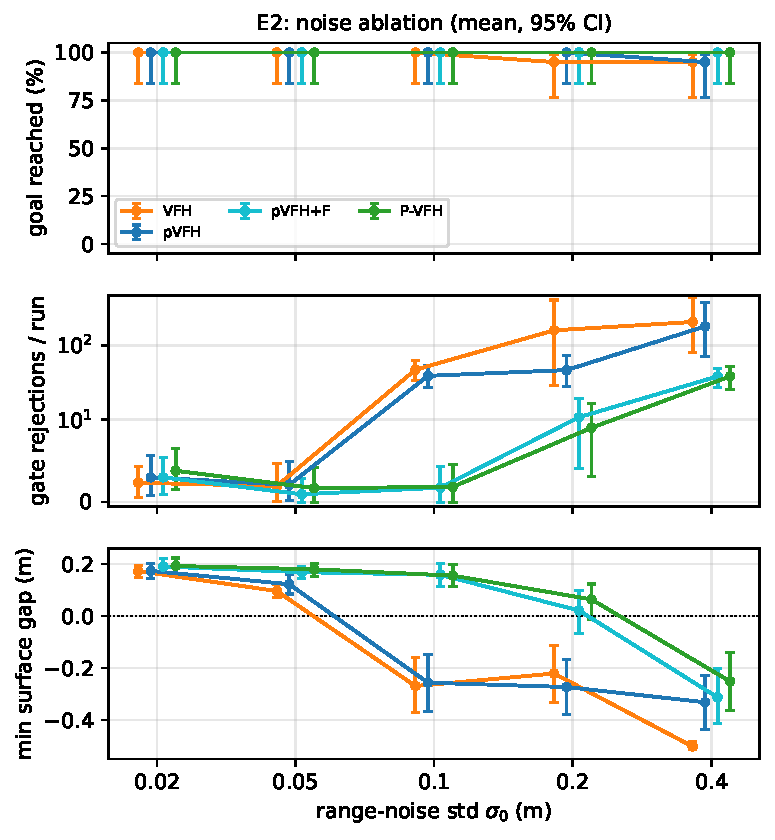
\includegraphics[width=0.74\textwidth]{figures/ablation_noise.pdf}
\caption{E2: reach rate, gate rejections and minimum surface gap against
$\sigma_0$, one line per law (points are dodged horizontally so coincident
intervals stay visible).}
\label{fig:e2}
\end{figure}

% AUTO-GENERATED by matlab/make_paper_figures.py -- do not edit
\begin{table}[H]
\centering\scriptsize
\begin{tabular}{@{}llrrrrrrr@{}}
\toprule
\textbf{Law} & \textbf{$\sigma_0$} & \textbf{Reach} [95\% CI, \%] & \textbf{Gate rej.} & \textbf{Static} & \textbf{Mover} & \textbf{Min gap (m)} [95\% CI] & \textbf{Eff.} & \textbf{Time (s)} \\
\midrule
VFH & 0.02 & 20/20 [84,100] & 2.4 & 0 & 0.0 & 0.17 [0.15,0.19] & 0.90 & 50 \\
VFH & 0.05 & 20/20 [84,100] & 1.9 & 0 & 0.0 & 0.10 [0.07,0.12] & 0.82 & 54 \\
VFH & 0.1 & 20/20 [84,100] & 46.9 & 0 & 26.9 & -0.27 [-0.37,-0.17] & 0.60 & 77 \\
VFH & 0.2 & 19/20 [76,99] & 158.7 & 0 & 14.3 & -0.22 [-0.33,-0.11] & 0.50 & 99 \\
VFH & 0.4 & 19/20 [76,99] & 205.6 & 0 & 39.2 & -0.50 [-0.51,-0.48] & 0.40 & 123 \\
\midrule
pVFH & 0.02 & 20/20 [84,100] & 3.0 & 0 & 0.0 & 0.17 [0.14,0.20] & 0.88 & 51 \\
pVFH & 0.05 & 20/20 [84,100] & 2.1 & 0 & 0.0 & 0.12 [0.08,0.16] & 0.82 & 53 \\
pVFH & 0.1 & 20/20 [84,100] & 38.8 & 0 & 21.8 & -0.26 [-0.36,-0.15] & 0.59 & 77 \\
pVFH & 0.2 & 20/20 [84,100] & 46.3 & 0 & 17.6 & -0.27 [-0.38,-0.17] & 0.50 & 89 \\
pVFH & 0.4 & 19/20 [76,99] & 179.7 & 0 & 36.0 & -0.33 [-0.44,-0.23] & 0.38 & 125 \\
\midrule
pVFH+F & 0.02 & 20/20 [84,100] & 3.0 & 0 & 0.0 & 0.19 [0.16,0.22] & 0.88 & 50 \\
pVFH+F & 0.05 & 20/20 [84,100] & 0.9 & 0 & 0.0 & 0.17 [0.14,0.19] & 0.86 & 51 \\
pVFH+F & 0.1 & 20/20 [84,100] & 1.8 & 0 & 0.0 & 0.16 [0.12,0.20] & 0.83 & 53 \\
pVFH+F & 0.2 & 20/20 [84,100] & 10.8 & 0 & 5.2 & 0.02 [-0.07,0.09] & 0.72 & 62 \\
pVFH+F & 0.4 & 20/20 [84,100] & 38.1 & 0 & 18.8 & -0.31 [-0.42,-0.20] & 0.53 & 84 \\
\midrule
P-VFH & 0.02 & 20/20 [84,100] & 3.8 & 0 & 0.0 & 0.19 [0.16,0.22] & 0.88 & 50 \\
P-VFH & 0.05 & 20/20 [84,100] & 1.7 & 0 & 0.0 & 0.18 [0.15,0.20] & 0.87 & 51 \\
P-VFH & 0.1 & 20/20 [84,100] & 1.9 & 0 & 0.0 & 0.16 [0.11,0.20] & 0.83 & 53 \\
P-VFH & 0.2 & 20/20 [84,100] & 9.0 & 0 & 1.4 & 0.06 [-0.01,0.12] & 0.72 & 63 \\
P-VFH & 0.4 & 20/20 [84,100] & 38.1 & 0 & 18.3 & -0.25 [-0.37,-0.14] & 0.56 & 81 \\
\bottomrule
\end{tabular}
\caption{E2, every cell. Reach: runs reaching the goal, Wilson interval. Gate rej.: mean steps per run in which the safety gate refused the commanded motion. Static: total static-contact steps over the cell (must be 0). Mover: mean steps per run in contact with a mover. Min gap: mean over runs of the per-run minimum surface gap, bootstrap interval. $\dagger$ = legacy pre-fix table, where this column is the old collision-step count.}
\label{tab:e2}
\end{table}


\paragraph{How to read E2.} The three panels share the x-axis. Top: the
fraction of runs that reached the goal --- a drop from 100\% is a law
starting to lose runs. Middle: gate rejections on a symmetric-log axis ---
the count of commands the supervisor refused. Bottom: the margin kept at
the worst moment of the run; the dotted line is contact. The prediction
above is supported only if the P-VFH line is at or above the deterministic
lines in the top and bottom panels and at or below them in the middle one,
with intervals that separate; overlapping intervals mean the experiment
did not resolve a difference at that noise level.

\subsection{Paired analysis}
\label{sec:paired}

\begin{figure}[H]
\centering
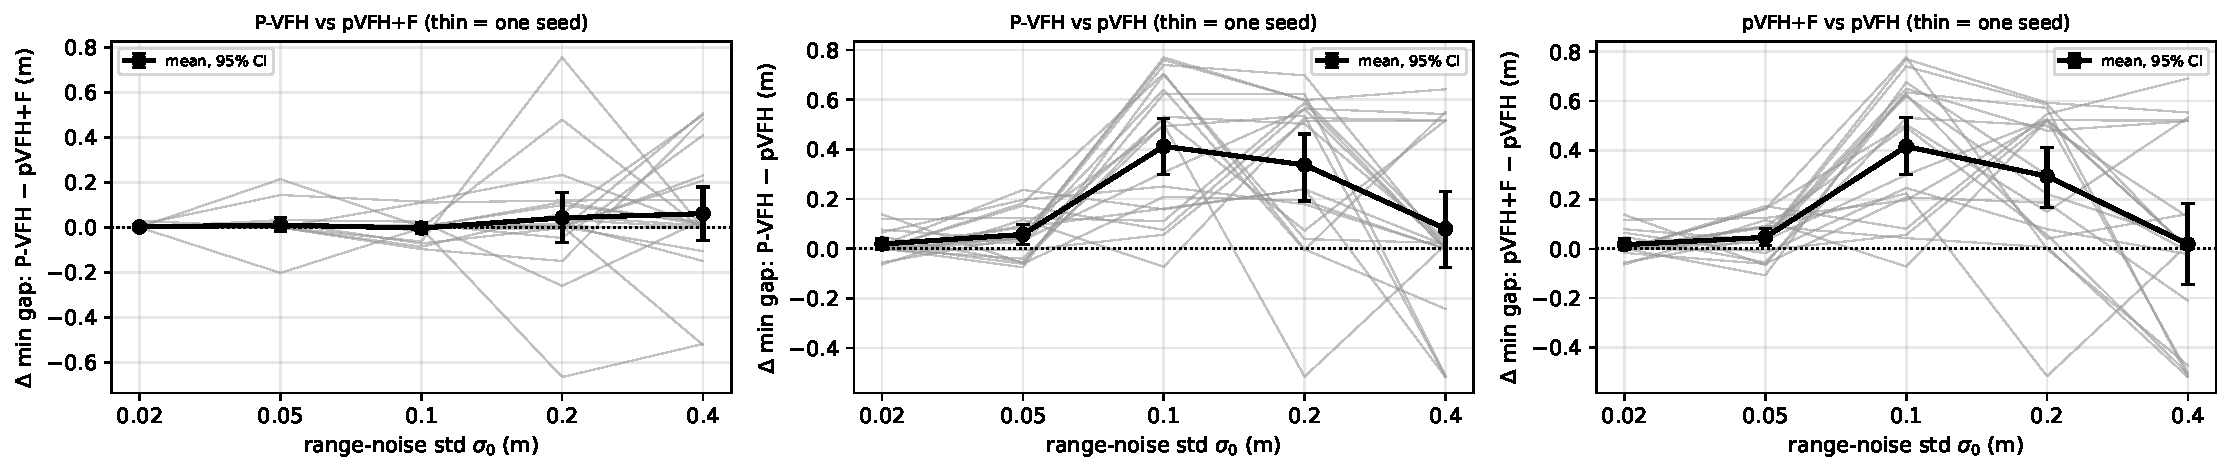
\includegraphics[width=\textwidth]{figures/paired_difference.pdf}
\caption{E2 paired by seed: difference in minimum surface gap per seed
(thin) and mean with 95\% interval (bold), for each step of the ladder:
P-VFH minus \code{pvfh\_filt} (the expected kernel alone), P-VFH minus
\code{pvfh} (filter and kernel), and \code{pvfh\_filt} minus \code{pvfh}
(the filter alone).}
\label{fig:paired}
\end{figure}

% AUTO-GENERATED by matlab/make_paper_figures.py -- do not edit
\begin{table}[H]
\centering\scriptsize
\begin{tabular}{@{}lllrrrrrrr@{}}
\toprule
\textbf{Exp.} & \textbf{World} & \textbf{vs} & $\sigma_0$ & $\Delta$\textbf{gap (m)} [95\% CI] & $p_W$ & $\Delta$\textbf{rej.} [95\% CI] & $p_W$ & \textbf{win/loss} & $p_M$ \\
\midrule
E2 & dynamic & pVFH+F & 0.02 & +0.00 [-0.00,+0.01] & 0.034 & +0.8 [+0.0,+2.4] & 0.180 & 0/0 & -- \\
E2 & dynamic & pVFH+F & 0.05 & +0.01 [-0.02,+0.04] & 0.152 & +0.8 [+0.0,+2.2] & 0.180 & 0/0 & -- \\
E2 & dynamic & pVFH+F & 0.1 & -0.00 [-0.03,+0.02] & 0.948 & +0.1 [+0.0,+0.3] & 0.317 & 0/0 & -- \\
E2 & dynamic & pVFH+F & 0.2 & +0.04 [-0.07,+0.16] & 0.165 & -1.8 [-11.0,+8.2] & 0.449 & 0/0 & -- \\
E2 & dynamic & pVFH+F & 0.4 & +0.06 [-0.07,+0.18] & 0.245 & +0.1 [-14.5,+14.5] & 0.896 & 0/0 & -- \\
E2 & dynamic & pVFH & 0.02 & +0.02 [-0.00,+0.04] & 0.076 & +0.8 [-2.0,+3.6] & 0.498 & 0/0 & -- \\
E2 & dynamic & pVFH & 0.05 & +0.06 [+0.02,+0.10] & 0.033 & -0.4 [-3.0,+2.2] & 0.389 & 0/0 & -- \\
E2 & dynamic & pVFH & 0.1 & +0.41 [+0.29,+0.53] & $<$0.001 & -36.9 [-49.5,-25.2] & $<$0.001 & 0/0 & -- \\
E2 & dynamic & pVFH & 0.2 & +0.34 [+0.19,+0.46] & $<$0.001 & -37.3 [-63.1,-17.9] & $<$0.001 & 0/0 & -- \\
E2 & dynamic & pVFH & 0.4 & +0.08 [-0.08,+0.24] & 0.083 & -141.6 [-346.9,-25.9] & 0.002 & 1/0 & 1.000 \\
E2 & dynamic & VFH & 0.02 & +0.02 [-0.01,+0.05] & 0.133 & +1.4 [-1.6,+4.4] & 0.297 & 0/0 & -- \\
E2 & dynamic & VFH & 0.05 & +0.08 [+0.05,+0.12] & $<$0.001 & -0.2 [-2.6,+2.4] & 0.596 & 0/0 & -- \\
E2 & dynamic & VFH & 0.1 & +0.43 [+0.30,+0.54] & $<$0.001 & -45.0 [-60.4,-31.3] & $<$0.001 & 0/0 & -- \\
E2 & dynamic & VFH & 0.2 & +0.29 [+0.15,+0.42] & $<$0.001 & -149.7 [-401.4,-17.1] & 0.001 & 1/0 & 1.000 \\
E2 & dynamic & VFH & 0.4 & +0.25 [+0.13,+0.37] & $<$0.001 & -167.4 [-407.6,-39.9] & $<$0.001 & 1/0 & 1.000 \\
E7 & maze & pVFH+F & 0.02 & -0.00 [-0.00,+0.00] & 1.000 & +0.0 [+0.0,+0.0] & -- & 0/0 & -- \\
E7 & maze & pVFH+F & 0.2 & -0.00 [-0.00,+0.00] & 1.000 & +0.0 [+0.0,+0.0] & -- & 0/0 & -- \\
E7 & maze & pVFH & 0.02 & -0.00 [-0.00,+0.00] & 0.064 & +0.0 [+0.0,+0.0] & -- & 0/0 & -- \\
E7 & maze & pVFH & 0.2 & +0.16 [+0.12,+0.20] & 0.002 & -2.2 [-5.7,-0.2] & 0.125 & 0/0 & -- \\
E7 & maze & VFH & 0.02 & -0.00 [-0.00,+0.00] & 0.064 & +0.0 [+0.0,+0.0] & -- & 0/0 & -- \\
E7 & maze & VFH & 0.2 & +0.14 [+0.09,+0.19] & 0.002 & -0.5 [-1.0,+0.0] & 0.250 & 0/0 & -- \\
E7 & plaza & pVFH+F & 0.02 & +0.01 [-0.15,+0.21] & 1.000 & -1.4 [-37.9,+25.4] & 0.875 & 0/0 & -- \\
E7 & plaza & pVFH+F & 0.2 & -0.05 [-0.14,+0.02] & 0.770 & +8.3 [-5.9,+23.2] & 0.461 & 0/0 & -- \\
E7 & plaza & pVFH & 0.02 & +0.00 [-0.30,+0.30] & 1.000 & -9.3 [-47.0,+26.5] & 0.367 & 0/0 & -- \\
E7 & plaza & pVFH & 0.2 & -0.00 [-0.15,+0.14] & 1.000 & +7.1 [-17.1,+32.9] & 0.625 & 0/0 & -- \\
E7 & plaza & VFH & 0.02 & +0.04 [-0.21,+0.28] & 0.432 & +2.2 [-30.6,+34.4] & 0.945 & 0/0 & -- \\
E7 & plaza & VFH & 0.2 & -0.02 [-0.18,+0.15] & 1.000 & +5.4 [-25.6,+33.4] & 0.770 & 0/0 & -- \\
E13 & 10 random layouts & pVFH+F & 0.02 & +0.00 [-0.00,+0.01] & 0.073 & -66.6 [-196.8,+0.0] & 0.104 & 1/0 & 1.000 \\
E13 & 10 random layouts & pVFH+F & 0.2 & -0.01 [-0.05,+0.04] & 0.209 & +1.6 [-4.7,+7.8] & 0.480 & 0/0 & -- \\
E13 & 10 random layouts & pVFH & 0.02 & +0.02 [-0.01,+0.07] & 0.152 & +6.7 [-5.7,+26.3] & 0.683 & 0/0 & -- \\
E13 & 10 random layouts & pVFH & 0.2 & +0.01 [-0.05,+0.09] & 0.490 & -99.4 [-253.3,-9.0] & 0.047 & 1/0 & 1.000 \\
E13 & 10 random layouts & VFH & 0.02 & +0.09 [+0.02,+0.17] & 0.584 & +9.8 [-10.0,+44.7] & 0.033 & 0/0 & -- \\
E13 & 10 random layouts & VFH & 0.2 & +0.12 [+0.04,+0.19] & 0.043 & -182.3 [-434.5,-14.6] & $<$0.001 & 2/0 & 0.500 \\
\bottomrule
\end{tabular}
\caption{Paired-seed tests, P-VFH minus the named deterministic law (positive $\Delta$gap and negative $\Delta$rej.\ favour P-VFH). $p_W$: two-sided Wilcoxon signed-rank on the per-seed differences; win/loss: seeds where only P-VFH / only the baseline reached the goal, $p_M$: exact McNemar (binomial) test on those discordant pairs. Intervals are percentile bootstrap. No multiplicity correction is applied; read the $p$-values with the number of rows in mind.}
\label{tab:stats}
\end{table}


\paragraph{How to read the paired results.} A point above zero favours the
first-named law at that noise level \emph{if} its interval excludes zero.
The left panel is the test of the expected kernel on its own; the right
panel is the test of the filter on its own. Whichever panel sits at zero
names the component that is not contributing. The thin lines show how
much individual seeds disagree; a mean carried by one or two seeds is weak
evidence however large it is. In Table~\ref{tab:stats}, the Wilcoxon
$p$-value addresses the size of the difference and the McNemar $p$-value
addresses reach; with this many rows, isolated values near 0.05 should not
be read as findings.

\subsection{E3 --- beam sweep}
\label{sec:e3}

\begin{figure}[H]
\centering
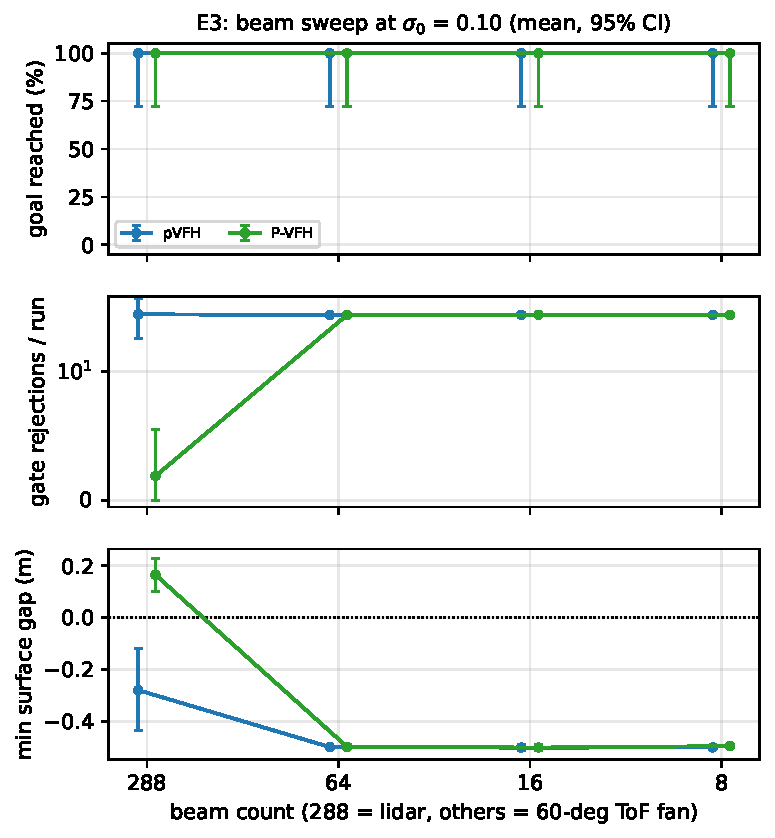
\includegraphics[width=0.74\textwidth]{figures/sweep_tof.pdf}
\caption{E3: the same three metrics against beam count at
$\sigma_0 = 0.10$~m (288 = lidar; 64, 16, 8 = $60^\circ$ body-fixed ToF
fan).}
\label{fig:e3}
\end{figure}

% AUTO-GENERATED by matlab/make_paper_figures.py -- do not edit
\begin{table}[H]
\centering\scriptsize
\begin{tabular}{@{}llrrrrrrr@{}}
\toprule
\textbf{Law} & \textbf{Sensor} & \textbf{Reach} [95\% CI, \%] & \textbf{Gate rej.} & \textbf{Static} & \textbf{Mover} & \textbf{Min gap (m)} [95\% CI] & \textbf{Eff.} & \textbf{Time (s)} \\
\midrule
pVFH & lidar-288 & 10/10 [72,100] & 30.8 & 0 & 16.1 & -0.28 [-0.44,-0.12] & 0.59 & 76 \\
pVFH & tof-64 & 10/10 [72,100] & 30.4 & 0 & 28.9 & -0.50 [-0.51,-0.49] & 1.00 & 48 \\
pVFH & tof-16 & 10/10 [72,100] & 30.5 & 0 & 29.0 & -0.50 [-0.51,-0.49] & 1.00 & 48 \\
pVFH & tof-8 & 10/10 [72,100] & 30.5 & 0 & 29.0 & -0.50 [-0.51,-0.49] & 1.00 & 48 \\
\midrule
P-VFH & lidar-288 & 10/10 [72,100] & 1.9 & 0 & 0.0 & 0.16 [0.10,0.22] & 0.83 & 53 \\
P-VFH & tof-64 & 10/10 [72,100] & 30.4 & 0 & 28.9 & -0.50 [-0.50,-0.49] & 1.00 & 48 \\
P-VFH & tof-16 & 10/10 [72,100] & 30.5 & 0 & 29.0 & -0.50 [-0.51,-0.49] & 1.00 & 48 \\
P-VFH & tof-8 & 10/10 [72,100] & 30.4 & 0 & 28.9 & -0.50 [-0.50,-0.49] & 1.00 & 48 \\
\bottomrule
\end{tabular}
\caption{E3. Reach: runs reaching the goal, Wilson interval. Gate rej.: mean steps per run in which the safety gate refused the commanded motion. Static: total static-contact steps over the cell (must be 0). Mover: mean steps per run in contact with a mover. Min gap: mean over runs of the per-run minimum surface gap, bootstrap interval. $\dagger$ = legacy pre-fix table, where this column is the old collision-step count.}
\label{tab:e3}
\end{table}


\paragraph{How to read E3.} Two things change between 288 and 64 beams ---
the fan narrows from $360^\circ$ to $60^\circ$ and the noise becomes
range-dependent --- so that step is a change of sensor, not only of
resolution; the 64~$\to$~16~$\to$~8 steps isolate resolution. A flat reach
line with a falling gap is the early warning: the law still arrives but
with less room. Watch the mover-contact column: a narrow forward fan cannot
see traffic approaching from the side or rear, and no steering law can
avoid what its sensor does not report.

\subsection{E4 --- formation shapes}
\label{sec:e4}

\begin{figure}[H]
\centering
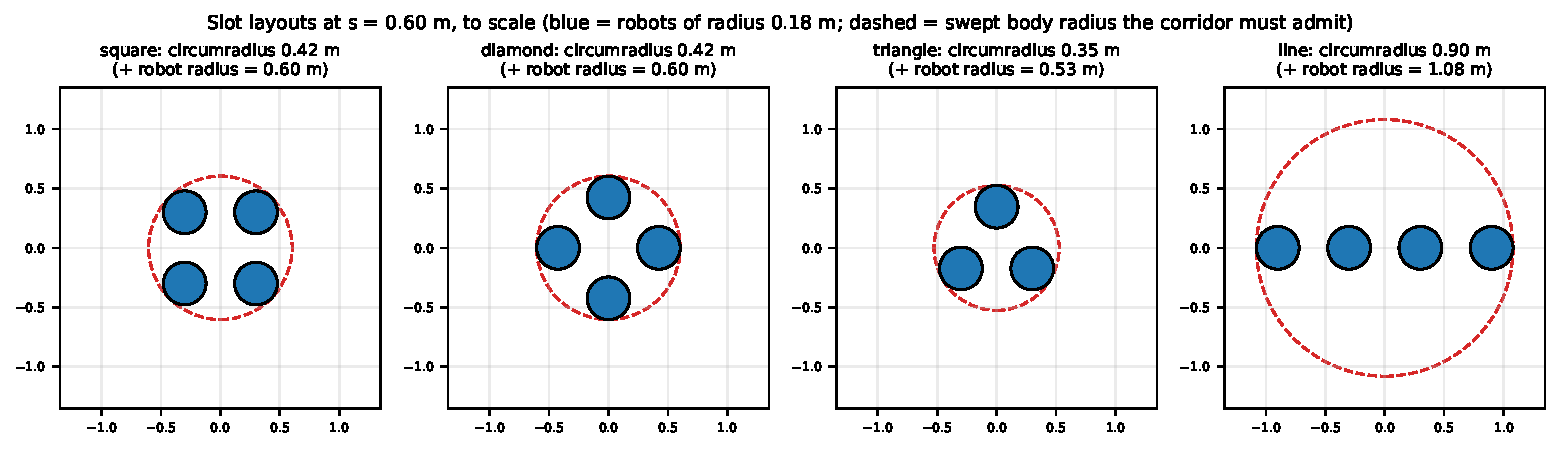
\includegraphics[width=0.95\textwidth]{figures/formation_sketch.pdf}
\caption{The four slot layouts at the E4/E5 spacing, to scale.}
\label{fig:fsketch}
\end{figure}

% AUTO-GENERATED by matlab/make_paper_figures.py -- do not edit
\begin{table}[H]
\centering\scriptsize
\begin{tabular}{@{}lrrrrrrr@{}}
\toprule
\textbf{Shape} & \textbf{Reach} [95\% CI, \%] & \textbf{Gate rej.} & \textbf{Static} & \textbf{Mover} & \textbf{Min gap (m)} [95\% CI] & \textbf{Eff.} & \textbf{Time (s)} \\
\midrule
square & 10/10 [72,100] & 0.0 & 0 & 0.0 & 0.62 [0.61,0.62] & 0.91 & 49 \\
diamond & 10/10 [72,100] & 0.0 & 0 & 0.0 & 0.49 [0.49,0.49] & 0.91 & 48 \\
triangle & 10/10 [72,100] & 0.0 & 0 & 0.0 & 0.58 [0.58,0.58] & 0.92 & 49 \\
line & 10/10 [72,100] & 10.7 & 0 & 1.8 & -0.02 [-0.11,0.03] & 0.52 & 84 \\
\bottomrule
\end{tabular}
\caption{E4. Reach: runs reaching the goal, Wilson interval. Gate rej.: mean steps per run in which the safety gate refused the commanded motion. Static: total static-contact steps over the cell (must be 0). Mover: mean steps per run in contact with a mover. Min gap: mean over runs of the per-run minimum surface gap, bootstrap interval. $\dagger$ = legacy pre-fix table, where this column is the old collision-step count.}
\label{tab:e4}
\end{table}


\begin{figure}[H]
\centering
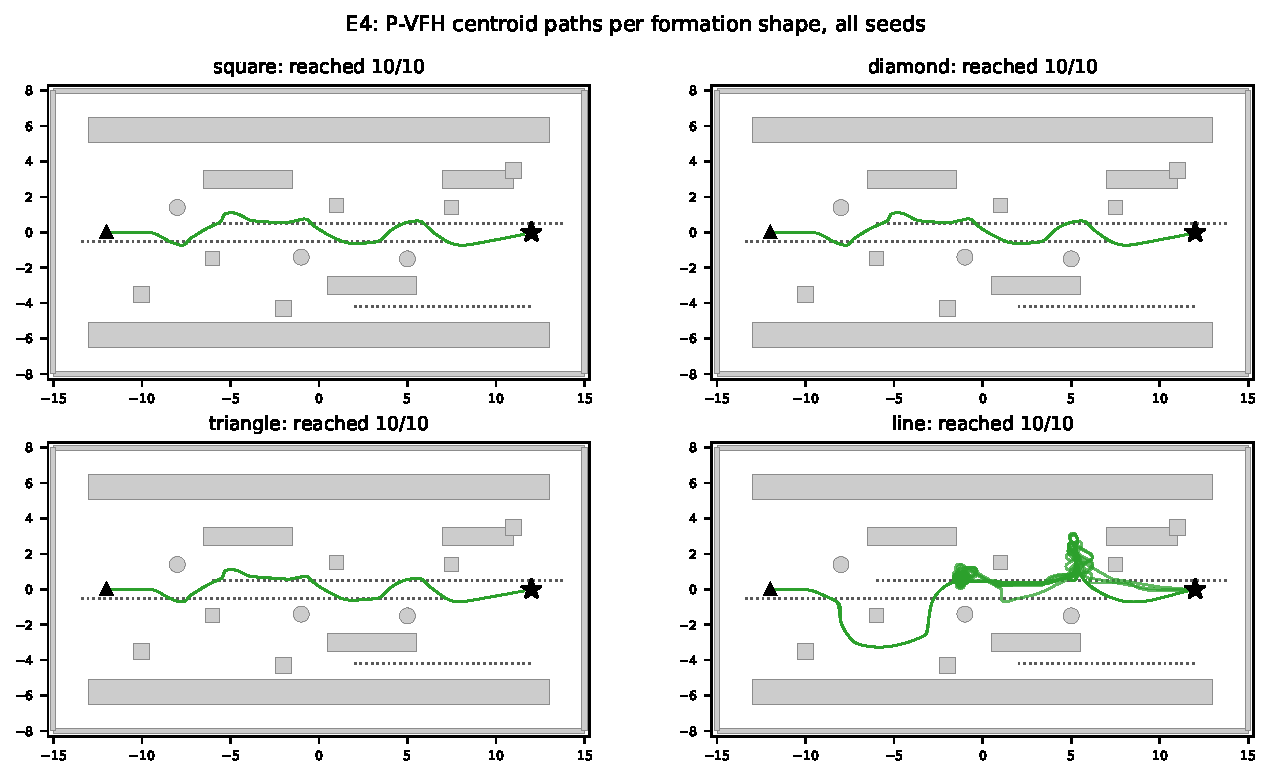
\includegraphics[width=\textwidth]{figures/formation_trails.pdf}
\caption{E4: P-VFH centroid paths for each shape, every seed.}
\label{fig:ftrails}
\end{figure}

\paragraph{How to read E4.} The corridor bottleneck is a half-width of
$1.22$~m. Square, diamond and triangle have swept radii well below it and
can turn anywhere. The line is different in kind: its swept radius also
fits, but it is a $2.16$~m-long body (four robots at $0.60$~m plus two
radii) that must \emph{rotate} to follow the chicane, and a rotation that
is blocked is a pivot the mission layer has to resolve. Expect the line to
be the slow shape; whether it is also a failing one is what the table
reports.

\subsection{E5 --- formation $\times$ steering law}
\label{sec:e5}

\begin{figure}[H]
\centering
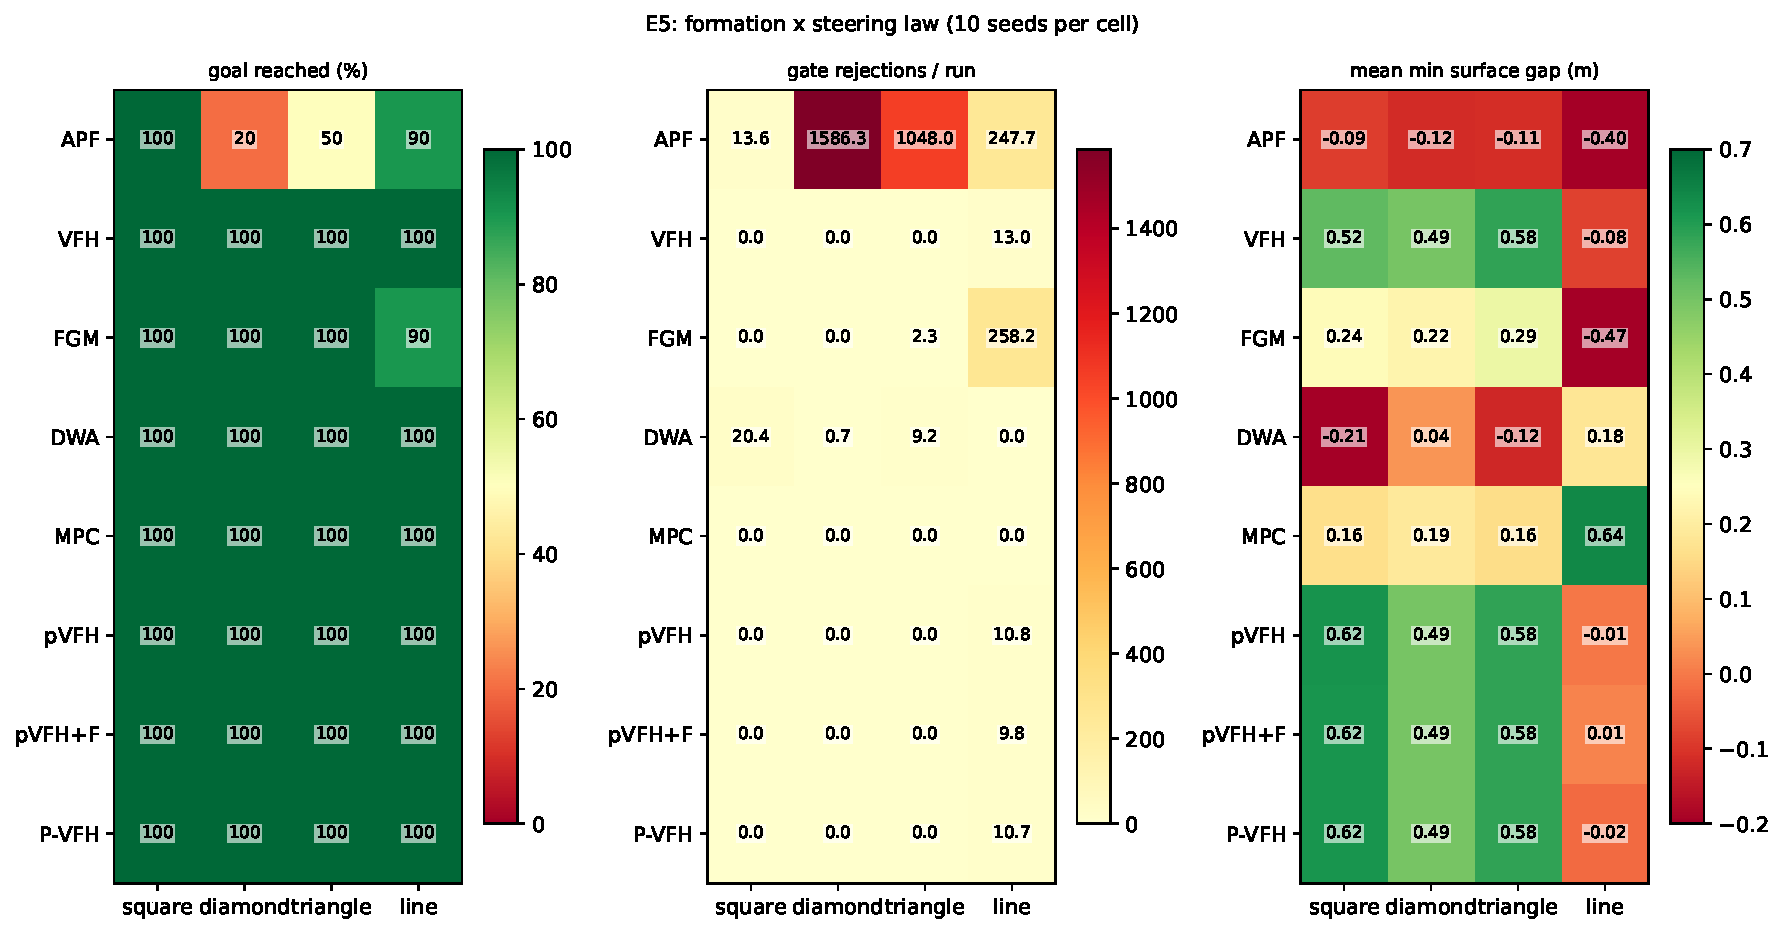
\includegraphics[width=\textwidth]{figures/e5_heatmap.pdf}
\caption{E5: reach rate, gate rejections and mean minimum surface gap per
(law, shape) cell.}
\label{fig:e5heat}
\end{figure}

% AUTO-GENERATED by matlab/make_paper_figures.py -- do not edit
\begin{table}[H]
\centering\scriptsize
\begin{tabular}{@{}llrrrrrrr@{}}
\toprule
\textbf{Law} & \textbf{Shape} & \textbf{Reach} [95\% CI, \%] & \textbf{Gate rej.} & \textbf{Static} & \textbf{Mover} & \textbf{Min gap (m)} [95\% CI] & \textbf{Eff.} & \textbf{Time (s)} \\
\midrule
APF & square & 10/10 [72,100] & 13.6 & 0 & 4.2 & -0.09 [-0.24,0.02] & 0.43 & 100 \\
APF & diamond & 2/10 [6,51] & 1586.3 & 0 & 6.1 & -0.12 [-0.26,0.00] & 0.23 & 268 \\
APF & triangle & 5/10 [24,76] & 1048.0 & 0 & 7.9 & -0.11 [-0.29,0.07] & 0.31 & 205 \\
APF & line & 9/10 [60,98] & 247.7 & 0 & 32.9 & -0.40 [-0.46,-0.35] & 0.31 & 150 \\
\midrule
VFH & square & 10/10 [72,100] & 0.0 & 0 & 0.0 & 0.52 [0.52,0.53] & 0.92 & 49 \\
VFH & diamond & 10/10 [72,100] & 0.0 & 0 & 0.0 & 0.49 [0.49,0.50] & 0.92 & 48 \\
VFH & triangle & 10/10 [72,100] & 0.0 & 0 & 0.0 & 0.58 [0.58,0.58] & 0.92 & 49 \\
VFH & line & 10/10 [72,100] & 13.0 & 0 & 4.1 & -0.08 [-0.23,0.02] & 0.51 & 85 \\
\midrule
FGM & square & 10/10 [72,100] & 0.0 & 0 & 0.0 & 0.24 [0.22,0.27] & 0.89 & 50 \\
FGM & diamond & 10/10 [72,100] & 0.0 & 0 & 0.0 & 0.22 [0.20,0.24] & 0.90 & 49 \\
FGM & triangle & 10/10 [72,100] & 2.3 & 0 & 2.0 & 0.29 [0.12,0.40] & 0.85 & 53 \\
FGM & line & 9/10 [60,98] & 258.2 & 0 & 30.2 & -0.47 [-0.49,-0.44] & 0.64 & 97 \\
\midrule
DWA & square & 10/10 [72,100] & 20.4 & 0 & 17.8 & -0.21 [-0.23,-0.19] & 0.96 & 51 \\
DWA & diamond & 10/10 [72,100] & 0.7 & 0 & 0.0 & 0.04 [0.03,0.04] & 0.96 & 49 \\
DWA & triangle & 10/10 [72,100] & 9.2 & 0 & 5.9 & -0.12 [-0.18,-0.07] & 0.97 & 50 \\
DWA & line & 10/10 [72,100] & 0.0 & 0 & 0.0 & 0.18 [0.16,0.19] & 0.91 & 51 \\
\midrule
MPC & square & 10/10 [72,100] & 0.0 & 0 & 0.0 & 0.16 [0.16,0.17] & 0.98 & 47 \\
MPC & diamond & 10/10 [72,100] & 0.0 & 0 & 0.0 & 0.19 [0.18,0.20] & 0.98 & 46 \\
MPC & triangle & 10/10 [72,100] & 0.0 & 0 & 0.0 & 0.16 [0.15,0.17] & 0.98 & 47 \\
MPC & line & 10/10 [72,100] & 0.0 & 0 & 0.0 & 0.64 [0.61,0.66] & 0.96 & 47 \\
\midrule
pVFH & square & 10/10 [72,100] & 0.0 & 0 & 0.0 & 0.62 [0.61,0.62] & 0.91 & 49 \\
pVFH & diamond & 10/10 [72,100] & 0.0 & 0 & 0.0 & 0.49 [0.49,0.50] & 0.92 & 48 \\
pVFH & triangle & 10/10 [72,100] & 0.0 & 0 & 0.0 & 0.58 [0.58,0.58] & 0.92 & 48 \\
pVFH & line & 10/10 [72,100] & 10.8 & 0 & 2.1 & -0.01 [-0.13,0.07] & 0.50 & 86 \\
\midrule
pVFH+F & square & 10/10 [72,100] & 0.0 & 0 & 0.0 & 0.62 [0.61,0.62] & 0.91 & 49 \\
pVFH+F & diamond & 10/10 [72,100] & 0.0 & 0 & 0.0 & 0.49 [0.49,0.49] & 0.91 & 48 \\
pVFH+F & triangle & 10/10 [72,100] & 0.0 & 0 & 0.0 & 0.58 [0.58,0.58] & 0.92 & 49 \\
pVFH+F & line & 10/10 [72,100] & 9.8 & 0 & 0.1 & 0.01 [-0.04,0.05] & 0.50 & 86 \\
\midrule
P-VFH & square & 10/10 [72,100] & 0.0 & 0 & 0.0 & 0.62 [0.61,0.62] & 0.91 & 49 \\
P-VFH & diamond & 10/10 [72,100] & 0.0 & 0 & 0.0 & 0.49 [0.49,0.49] & 0.91 & 48 \\
P-VFH & triangle & 10/10 [72,100] & 0.0 & 0 & 0.0 & 0.58 [0.58,0.58] & 0.92 & 49 \\
P-VFH & line & 10/10 [72,100] & 10.7 & 0 & 1.8 & -0.02 [-0.11,0.03] & 0.52 & 84 \\
\bottomrule
\end{tabular}
\caption{E5, every cell. Reach: runs reaching the goal, Wilson interval. Gate rej.: mean steps per run in which the safety gate refused the commanded motion. Static: total static-contact steps over the cell (must be 0). Mover: mean steps per run in contact with a mover. Min gap: mean over runs of the per-run minimum surface gap, bootstrap interval. $\dagger$ = legacy pre-fix table, where this column is the old collision-step count.}
\label{tab:e5}
\end{table}


\begin{figure}[H]
\centering
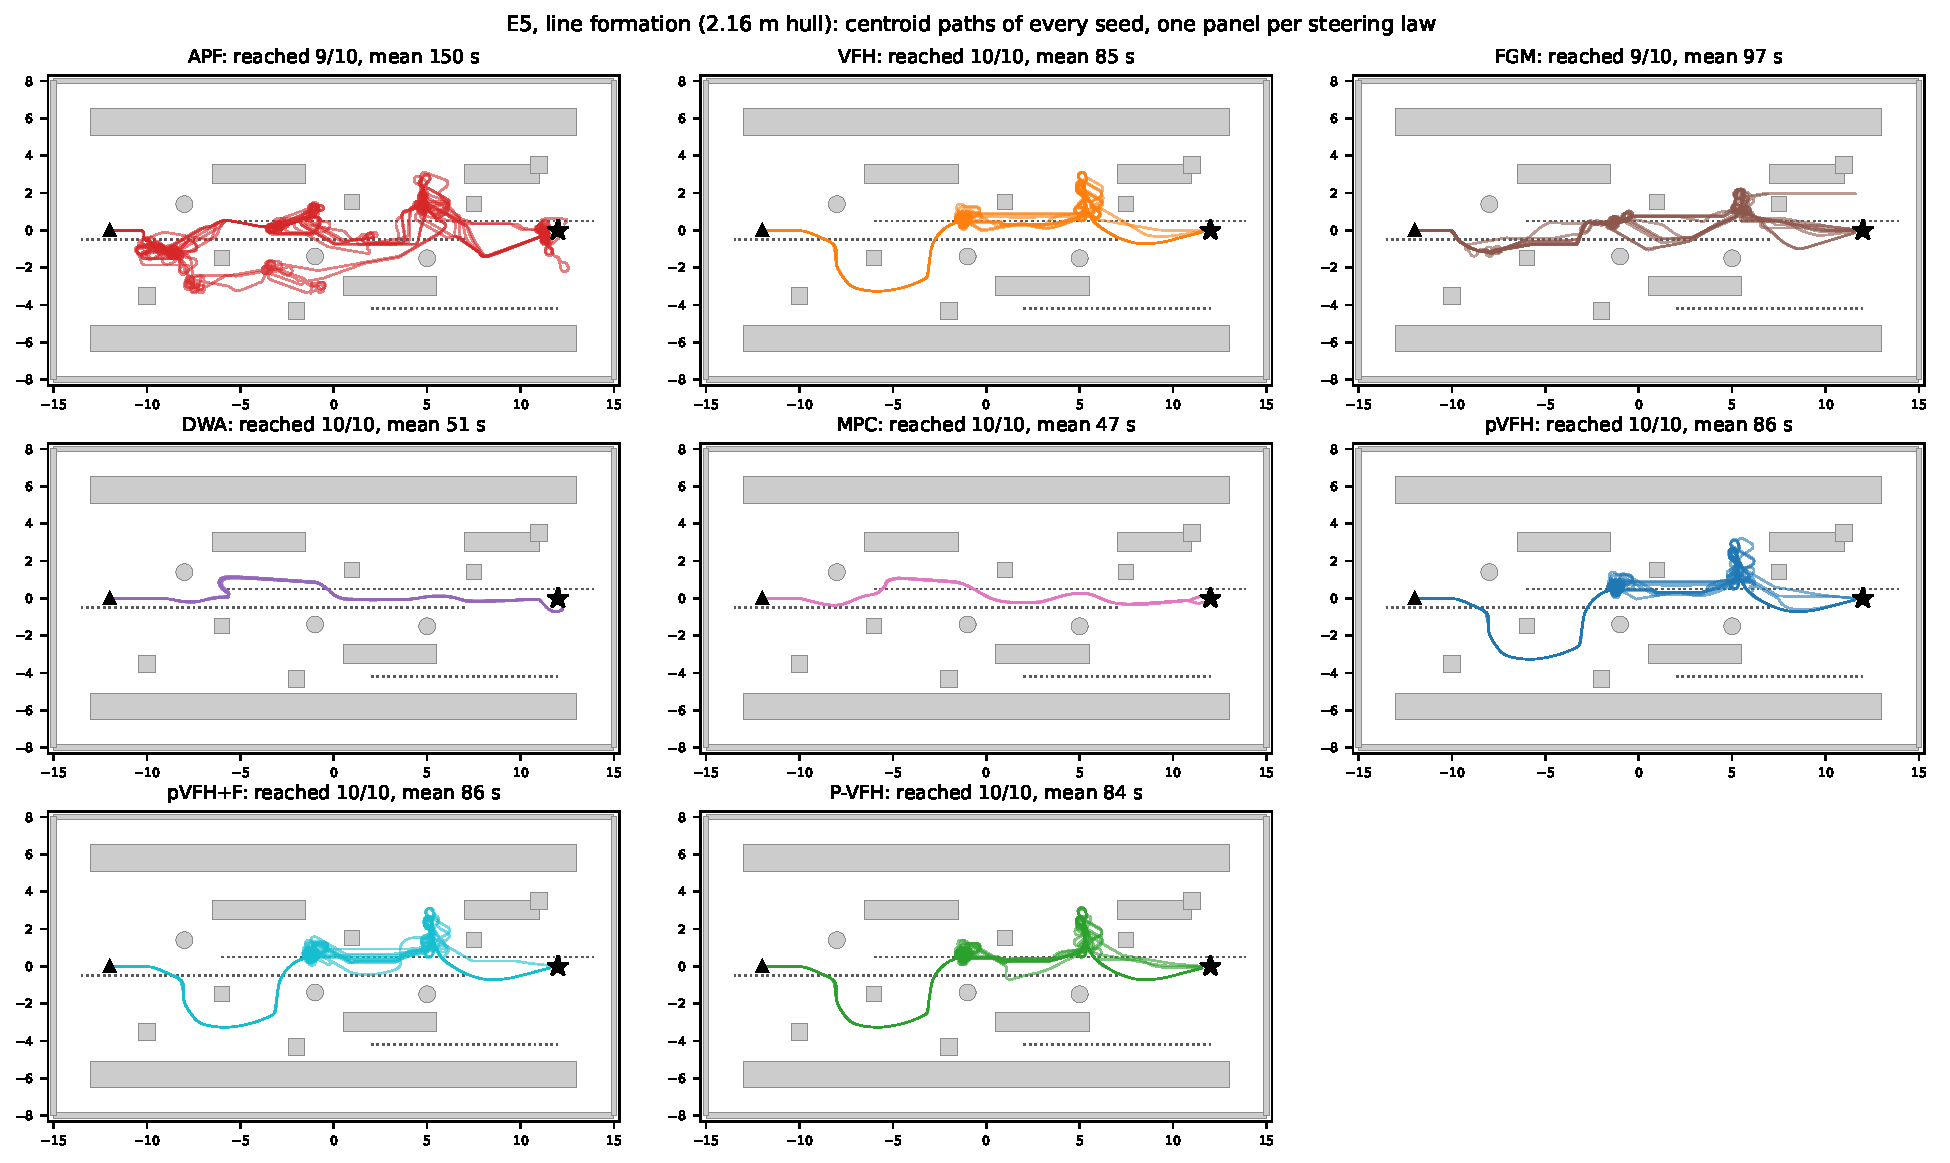
\includegraphics[width=\textwidth]{figures/e5_line_anatomy.pdf}
\caption{E5, line formation: every seed's path, one panel per law.}
\label{fig:e5anatomy}
\end{figure}

\begin{figure}[H]
\centering
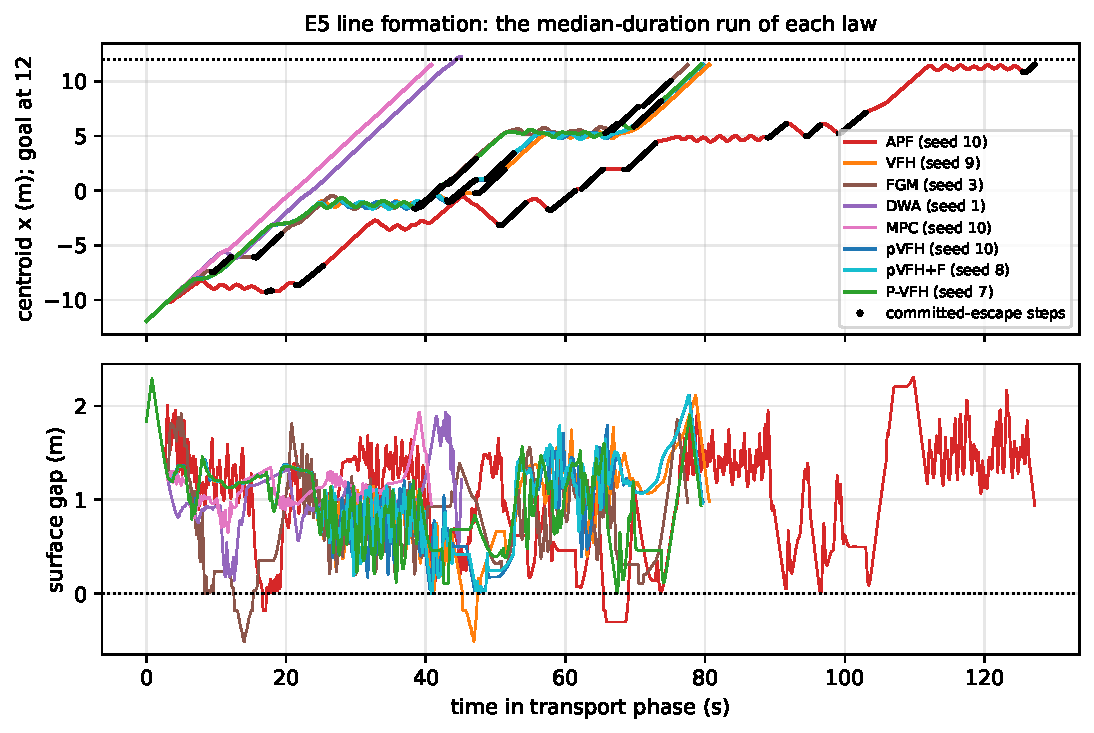
\includegraphics[width=0.85\textwidth]{figures/e5_stall_timeseries.pdf}
\caption{E5, line formation: progress and surface gap over time for the
median-duration run of each law. Black dots mark steps taken under a
committed escape.}
\label{fig:e5stall}
\end{figure}

\paragraph{How to read E5.} Read the heatmaps in two directions.
\emph{Across a row} (fixed law): does the shape matter to this law?
\emph{Down a column} (fixed shape): does the law matter for this shape? A
column in which some cells fail and others do not is an \emph{interaction}
--- the effect of the law depends on the shape --- which neither E1 nor E4
can show. In the time series, a flat stretch of the progress trace is a
stall: if the gap trace below it is near zero the body is jammed against
something; if the gap is comfortably positive it is a pivot that either
the steering law or a committed escape (black dots) must end. The run for
each law is chosen by a rule (median mission time), not by hand.

\subsection{E6 --- matched sensor comparison}
\label{sec:e6}

\begin{figure}[H]
\centering
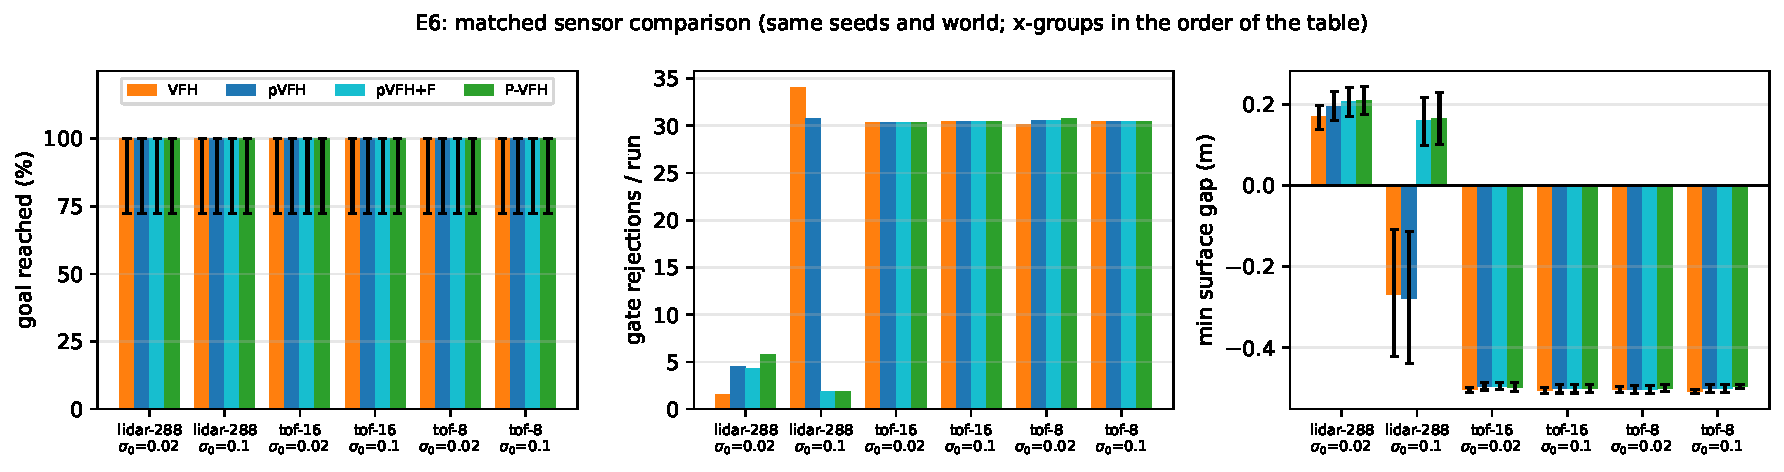
\includegraphics[width=\textwidth]{figures/e6_sensor.pdf}
\caption{E6: reach, gate rejections and gap by sensor configuration and
law.}
\label{fig:e6}
\end{figure}

% AUTO-GENERATED by matlab/make_paper_figures.py -- do not edit
\begin{table}[H]
\centering\scriptsize
\begin{tabular}{@{}lllrrrrrrr@{}}
\toprule
\textbf{Sensor} & \textbf{$\sigma_0$} & \textbf{Law} & \textbf{Reach} [95\% CI, \%] & \textbf{Gate rej.} & \textbf{Static} & \textbf{Mover} & \textbf{Min gap (m)} [95\% CI] & \textbf{Eff.} & \textbf{Time (s)} \\
\midrule
lidar-288 & 0.02 & VFH & 10/10 [72,100] & 1.6 & 0 & 0.0 & 0.17 [0.14,0.20] & 0.90 & 49 \\
lidar-288 & 0.02 & pVFH & 10/10 [72,100] & 4.5 & 0 & 0.0 & 0.19 [0.16,0.23] & 0.89 & 50 \\
lidar-288 & 0.02 & pVFH+F & 10/10 [72,100] & 4.3 & 0 & 0.0 & 0.21 [0.17,0.24] & 0.89 & 50 \\
lidar-288 & 0.02 & P-VFH & 10/10 [72,100] & 5.8 & 0 & 0.0 & 0.21 [0.18,0.24] & 0.89 & 50 \\
lidar-288 & 0.1 & VFH & 10/10 [72,100] & 34.1 & 0 & 15.3 & -0.27 [-0.42,-0.11] & 0.60 & 76 \\
lidar-288 & 0.1 & pVFH & 10/10 [72,100] & 30.8 & 0 & 16.1 & -0.28 [-0.43,-0.12] & 0.59 & 76 \\
lidar-288 & 0.1 & pVFH+F & 10/10 [72,100] & 1.9 & 0 & 0.0 & 0.16 [0.10,0.22] & 0.83 & 53 \\
lidar-288 & 0.1 & P-VFH & 10/10 [72,100] & 1.9 & 0 & 0.0 & 0.16 [0.10,0.23] & 0.83 & 53 \\
\midrule
tof-16 & 0.02 & VFH & 10/10 [72,100] & 30.3 & 0 & 29.0 & -0.50 [-0.51,-0.50] & 1.00 & 48 \\
tof-16 & 0.02 & pVFH & 10/10 [72,100] & 30.3 & 0 & 28.9 & -0.50 [-0.50,-0.49] & 1.00 & 48 \\
tof-16 & 0.02 & pVFH+F & 10/10 [72,100] & 30.3 & 0 & 28.9 & -0.50 [-0.50,-0.49] & 1.00 & 48 \\
tof-16 & 0.02 & P-VFH & 10/10 [72,100] & 30.3 & 0 & 28.9 & -0.50 [-0.51,-0.49] & 1.00 & 48 \\
tof-16 & 0.1 & VFH & 10/10 [72,100] & 30.4 & 0 & 29.0 & -0.51 [-0.51,-0.50] & 1.00 & 48 \\
tof-16 & 0.1 & pVFH & 10/10 [72,100] & 30.5 & 0 & 29.0 & -0.50 [-0.51,-0.49] & 1.00 & 48 \\
tof-16 & 0.1 & pVFH+F & 10/10 [72,100] & 30.5 & 0 & 29.0 & -0.50 [-0.51,-0.49] & 1.00 & 48 \\
tof-16 & 0.1 & P-VFH & 10/10 [72,100] & 30.5 & 0 & 29.0 & -0.50 [-0.51,-0.49] & 1.00 & 48 \\
\midrule
tof-8 & 0.02 & VFH & 10/10 [72,100] & 30.1 & 0 & 29.0 & -0.50 [-0.51,-0.49] & 1.00 & 48 \\
tof-8 & 0.02 & pVFH & 10/10 [72,100] & 30.6 & 0 & 29.0 & -0.50 [-0.51,-0.49] & 1.00 & 48 \\
tof-8 & 0.02 & pVFH+F & 10/10 [72,100] & 30.6 & 0 & 29.0 & -0.50 [-0.51,-0.49] & 1.00 & 48 \\
tof-8 & 0.02 & P-VFH & 10/10 [72,100] & 30.8 & 0 & 29.0 & -0.50 [-0.51,-0.49] & 1.00 & 48 \\
tof-8 & 0.1 & VFH & 10/10 [72,100] & 30.4 & 0 & 29.2 & -0.51 [-0.51,-0.50] & 1.00 & 48 \\
tof-8 & 0.1 & pVFH & 10/10 [72,100] & 30.5 & 0 & 29.0 & -0.50 [-0.51,-0.49] & 1.00 & 48 \\
tof-8 & 0.1 & pVFH+F & 10/10 [72,100] & 30.5 & 0 & 29.0 & -0.50 [-0.51,-0.49] & 1.00 & 48 \\
tof-8 & 0.1 & P-VFH & 10/10 [72,100] & 30.4 & 0 & 28.9 & -0.50 [-0.50,-0.49] & 1.00 & 48 \\
\bottomrule
\end{tabular}
\caption{E6, every cell. Reach: runs reaching the goal, Wilson interval. Gate rej.: mean steps per run in which the safety gate refused the commanded motion. Static: total static-contact steps over the cell (must be 0). Mover: mean steps per run in contact with a mover. Min gap: mean over runs of the per-run minimum surface gap, bootstrap interval. $\dagger$ = legacy pre-fix table, where this column is the old collision-step count.}
\label{tab:e6}
\end{table}


\begin{figure}[H]
\centering
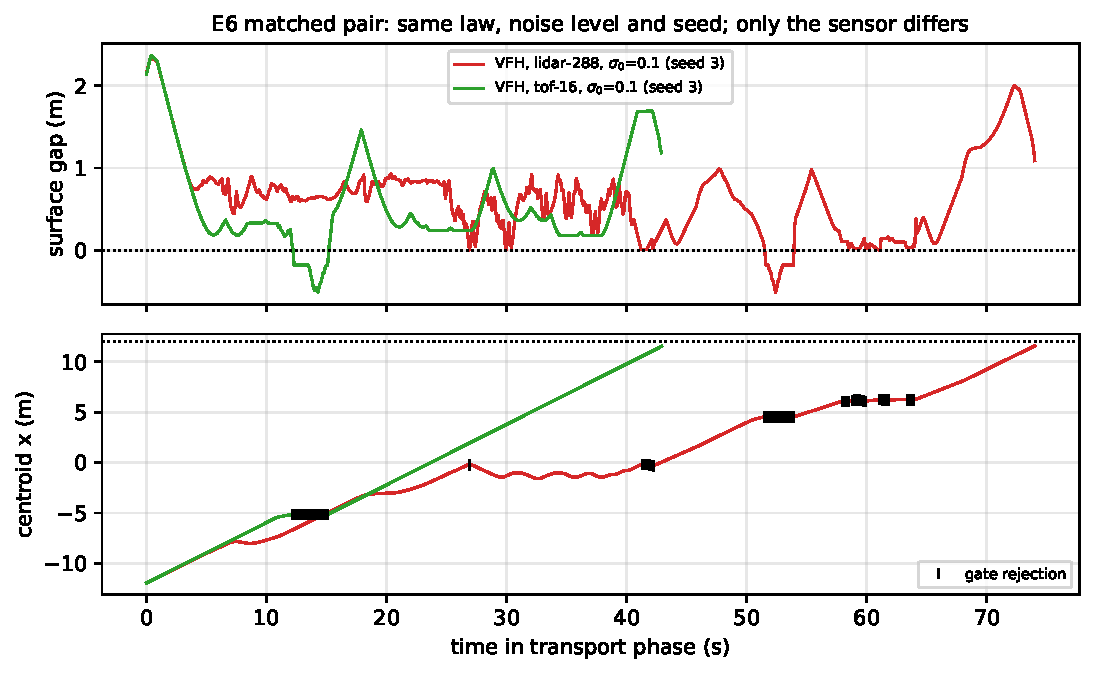
\includegraphics[width=0.85\textwidth]{figures/e6_timeseries.pdf}
\caption{E6 matched pair: deterministic VFH at the higher noise level on
lidar-288 and on tof-16, same seed (the lidar cell's worst seed by gate
rejections).}
\label{fig:e6ts}
\end{figure}

\paragraph{How to read E6.} Within an x-group the bars differ only by law;
across groups only the sensor changes. The lidar cells reuse the E2
simulations of the first ten seeds at the same $\sigma_0$ (each
configuration is run once), so they must agree with Table~\ref{tab:e2} up
to the ten extra seeds E2 carries. The two caveats of E3 apply: a narrow fan reacts to
fewer side obstacles, which can look like better behaviour, and is blind
to side and rear traffic, which shows up as mover contacts.

\subsection{E7 --- other environments}
\label{sec:e7}

The warehouse is one layout. E7 repeats the eight-law comparison at a low and
a high noise level in two further worlds with the same bounds, start and
goal: an \textbf{open plaza} (fourteen compact obstacles, no aisles,
traffic that \emph{crosses} the route) and a \textbf{serpentine maze}
(three baffles with alternating $3.25$~m gates, forcing four turns of about
$90^\circ$). In the maze every law is given the same four-waypoint global
route: a reactive law has no reason to drive away from the goal toward a
gate, so the experiment tests local steering along a given route, not
global planning.

\begin{figure}[H]
\centering
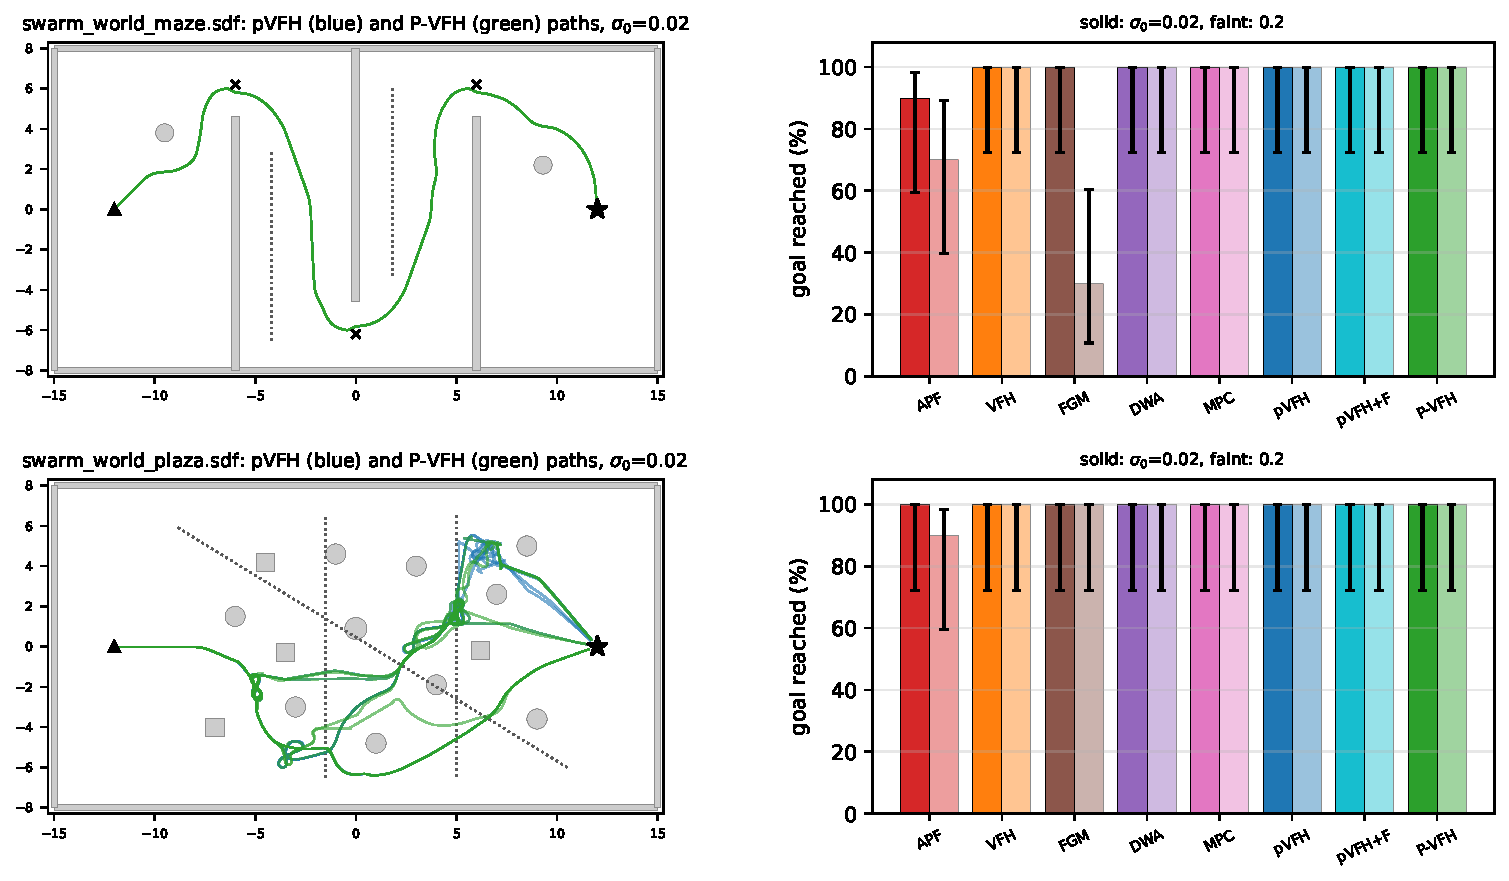
\includegraphics[width=\textwidth]{figures/e7_environments.pdf}
\caption{E7. Left: the worlds with the paths of the two horizon-equipped
histogram laws at the low noise level. Right: reach rate per law (solid:
low noise; faint: high noise).}
\label{fig:e7}
\end{figure}

% AUTO-GENERATED by matlab/make_paper_figures.py -- do not edit
\begin{table}[H]
\centering\scriptsize
\begin{tabular}{@{}lllrrrrrrr@{}}
\toprule
\textbf{World} & \textbf{$\sigma_0$} & \textbf{Law} & \textbf{Reach} [95\% CI, \%] & \textbf{Gate rej.} & \textbf{Static} & \textbf{Mover} & \textbf{Min gap (m)} [95\% CI] & \textbf{Eff.} & \textbf{Time (s)} \\
\midrule
maze & 0.02 & APF & 9/10 [60,98] & 199.8 & 0 & 0.0 & 0.04 [0.01,0.08] & 0.23 & 198 \\
maze & 0.02 & VFH & 10/10 [72,100] & 0.0 & 0 & 0.0 & 0.27 [0.27,0.27] & 0.50 & 84 \\
maze & 0.02 & FGM & 10/10 [72,100] & 12.4 & 0 & 0.0 & 0.01 [0.00,0.01] & 0.40 & 108 \\
maze & 0.02 & DWA & 10/10 [72,100] & 0.0 & 0 & 0.0 & 0.13 [0.12,0.13] & 0.51 & 83 \\
maze & 0.02 & MPC & 10/10 [72,100] & 0.0 & 0 & 0.0 & 0.28 [0.27,0.29] & 0.52 & 81 \\
maze & 0.02 & pVFH & 10/10 [72,100] & 0.0 & 0 & 0.0 & 0.27 [0.27,0.27] & 0.50 & 84 \\
maze & 0.02 & pVFH+F & 10/10 [72,100] & 0.0 & 0 & 0.0 & 0.27 [0.26,0.27] & 0.50 & 84 \\
maze & 0.02 & P-VFH & 10/10 [72,100] & 0.0 & 0 & 0.0 & 0.27 [0.26,0.27] & 0.50 & 84 \\
maze & 0.2 & APF & 7/10 [40,89] & 1341.1 & 0 & 0.0 & 0.01 [0.00,0.01] & 0.15 & 368 \\
maze & 0.2 & VFH & 10/10 [72,100] & 0.5 & 0 & 0.0 & 0.10 [0.06,0.15] & 0.40 & 105 \\
maze & 0.2 & FGM & 3/10 [11,60] & 3386.4 & 0 & 0.0 & 0.01 [0.00,0.03] & 0.15 & 534 \\
maze & 0.2 & DWA & 10/10 [72,100] & 0.0 & 0 & 0.0 & 0.33 [0.32,0.34] & 0.50 & 86 \\
maze & 0.2 & MPC & 10/10 [72,100] & 0.0 & 0 & 0.0 & 0.45 [0.43,0.47] & 0.50 & 84 \\
maze & 0.2 & pVFH & 10/10 [72,100] & 2.2 & 0 & 0.0 & 0.08 [0.04,0.12] & 0.40 & 105 \\
maze & 0.2 & pVFH+F & 10/10 [72,100] & 0.0 & 0 & 0.0 & 0.24 [0.23,0.25] & 0.50 & 84 \\
maze & 0.2 & P-VFH & 10/10 [72,100] & 0.0 & 0 & 0.0 & 0.24 [0.23,0.25] & 0.50 & 84 \\
\midrule
plaza & 0.02 & APF & 10/10 [72,100] & 85.3 & 0 & 25.5 & -0.33 [-0.47,-0.17] & 0.41 & 110 \\
plaza & 0.02 & VFH & 10/10 [72,100] & 33.2 & 0 & 18.3 & -0.17 [-0.34,-0.01] & 0.58 & 79 \\
plaza & 0.02 & FGM & 10/10 [72,100] & 63.8 & 0 & 27.5 & -0.35 [-0.50,-0.20] & 0.54 & 84 \\
plaza & 0.02 & DWA & 10/10 [72,100] & 27.0 & 0 & 14.7 & -0.01 [-0.15,0.09] & 0.74 & 65 \\
plaza & 0.02 & MPC & 10/10 [72,100] & 0.0 & 0 & 0.0 & 0.09 [0.05,0.13] & 0.88 & 50 \\
plaza & 0.02 & pVFH & 10/10 [72,100] & 44.7 & 0 & 25.9 & -0.13 [-0.32,0.06] & 0.55 & 88 \\
plaza & 0.02 & pVFH+F & 10/10 [72,100] & 36.8 & 0 & 15.2 & -0.14 [-0.32,0.04] & 0.55 & 84 \\
plaza & 0.02 & P-VFH & 10/10 [72,100] & 35.4 & 0 & 14.8 & -0.13 [-0.32,0.06] & 0.59 & 79 \\
plaza & 0.2 & APF & 9/10 [60,98] & 251.7 & 0 & 27.3 & -0.34 [-0.50,-0.16] & 0.34 & 144 \\
plaza & 0.2 & VFH & 10/10 [72,100] & 58.6 & 0 & 22.9 & -0.21 [-0.35,-0.08] & 0.54 & 84 \\
plaza & 0.2 & FGM & 10/10 [72,100] & 53.3 & 0 & 21.2 & -0.24 [-0.39,-0.10] & 0.51 & 88 \\
plaza & 0.2 & DWA & 10/10 [72,100] & 5.4 & 0 & 0.0 & 0.17 [0.09,0.25] & 0.69 & 65 \\
plaza & 0.2 & MPC & 10/10 [72,100] & 0.2 & 0 & 0.0 & 0.25 [0.12,0.38] & 0.75 & 58 \\
plaza & 0.2 & pVFH & 10/10 [72,100] & 56.9 & 0 & 16.9 & -0.22 [-0.35,-0.10] & 0.54 & 84 \\
plaza & 0.2 & pVFH+F & 10/10 [72,100] & 55.7 & 0 & 18.0 & -0.17 [-0.31,-0.05] & 0.53 & 87 \\
plaza & 0.2 & P-VFH & 10/10 [72,100] & 64.0 & 0 & 28.6 & -0.23 [-0.36,-0.09] & 0.53 & 87 \\
\bottomrule
\end{tabular}
\caption{E7, every cell. Reach: runs reaching the goal, Wilson interval. Gate rej.: mean steps per run in which the safety gate refused the commanded motion. Static: total static-contact steps over the cell (must be 0). Mover: mean steps per run in contact with a mover. Min gap: mean over runs of the per-run minimum surface gap, bootstrap interval. $\dagger$ = legacy pre-fix table, where this column is the old collision-step count.}
\label{tab:e7}
\end{table}


\paragraph{How to read E7.} The question is whether the \emph{ordering} of
the laws seen in the warehouse persists, not whether the absolute values
do. Three layouts are still a small sample of the space of environments,
and all three were designed by the authors; E7 widens the evidence, it
does not make it general.

\subsection{E8 --- traffic speed}
\label{sec:e8}

\begin{figure}[H]
\centering
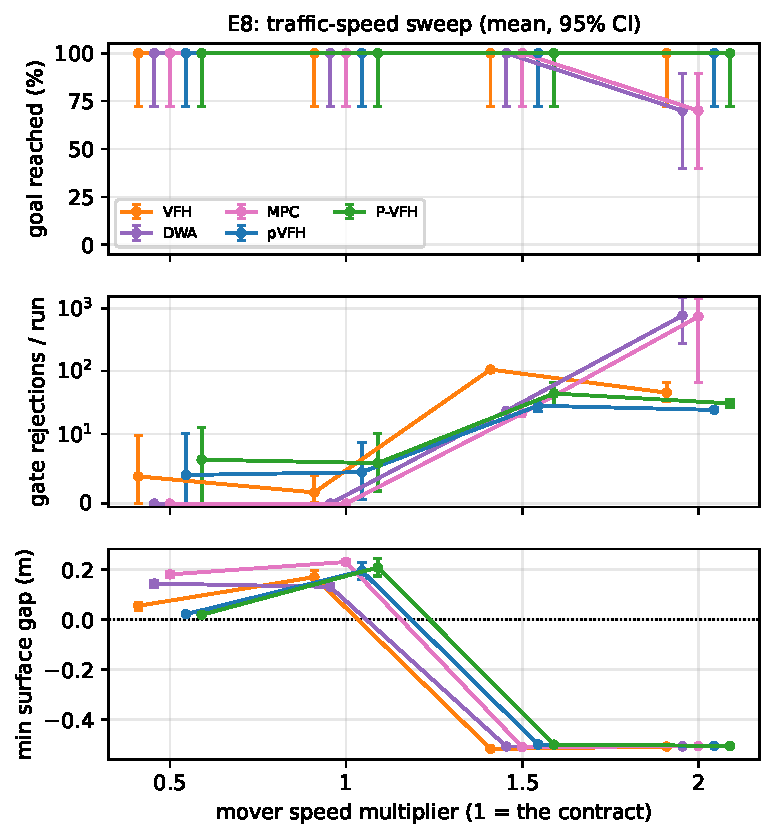
\includegraphics[width=0.74\textwidth]{figures/e8_traffic.pdf}
\caption{E8: the three metrics against the mover-speed multiplier.}
\label{fig:e8}
\end{figure}

% AUTO-GENERATED by matlab/make_paper_figures.py -- do not edit
\begin{table}[H]
\centering\scriptsize
\begin{tabular}{@{}llrrrrrrr@{}}
\toprule
\textbf{Law} & \textbf{Mover speed x} & \textbf{Reach} [95\% CI, \%] & \textbf{Gate rej.} & \textbf{Static} & \textbf{Mover} & \textbf{Min gap (m)} [95\% CI] & \textbf{Eff.} & \textbf{Time (s)} \\
\midrule
VFH & 0.5 & 10/10 [72,100] & 3.9 & 0 & 0.0 & 0.06 [0.04,0.07] & 0.88 & 50 \\
VFH & 1 & 10/10 [72,100] & 1.6 & 0 & 0.0 & 0.17 [0.14,0.20] & 0.90 & 49 \\
VFH & 1.5 & 10/10 [72,100] & 106.1 & 0 & 92.2 & -0.52 [-0.52,-0.51] & 0.90 & 61 \\
VFH & 2 & 10/10 [72,100] & 45.3 & 0 & 30.9 & -0.51 [-0.51,-0.50] & 0.81 & 59 \\
\midrule
DWA & 0.5 & 10/10 [72,100] & 0.0 & 0 & 0.0 & 0.14 [0.13,0.16] & 0.94 & 49 \\
DWA & 1 & 10/10 [72,100] & 0.0 & 0 & 0.0 & 0.13 [0.12,0.14] & 0.91 & 50 \\
DWA & 1.5 & 10/10 [72,100] & 23.3 & 0 & 19.7 & -0.51 [-0.51,-0.50] & 0.96 & 50 \\
DWA & 2 & 7/10 [40,89] & 770.4 & 0 & 35.9 & -0.51 [-0.51,-0.50] & 0.75 & 134 \\
\midrule
MPC & 0.5 & 10/10 [72,100] & 0.0 & 0 & 0.0 & 0.18 [0.17,0.19] & 0.95 & 47 \\
MPC & 1 & 10/10 [72,100] & 0.0 & 0 & 0.0 & 0.23 [0.22,0.24] & 0.97 & 46 \\
MPC & 1.5 & 10/10 [72,100] & 21.3 & 0 & 19.7 & -0.51 [-0.51,-0.51] & 0.98 & 48 \\
MPC & 2 & 7/10 [40,89] & 740.7 & 0 & 35.6 & -0.51 [-0.51,-0.50] & 0.68 & 133 \\
\midrule
pVFH & 0.5 & 10/10 [72,100] & 4.1 & 0 & 0.0 & 0.02 [0.02,0.03] & 0.88 & 50 \\
pVFH & 1 & 10/10 [72,100] & 4.5 & 0 & 0.0 & 0.19 [0.16,0.23] & 0.89 & 50 \\
pVFH & 1.5 & 10/10 [72,100] & 28.1 & 0 & 20.0 & -0.50 [-0.51,-0.49] & 0.68 & 66 \\
pVFH & 2 & 10/10 [72,100] & 24.1 & 0 & 15.7 & -0.50 [-0.51,-0.50] & 0.80 & 58 \\
\midrule
P-VFH & 0.5 & 10/10 [72,100] & 6.3 & 0 & 0.0 & 0.02 [0.01,0.03] & 0.88 & 51 \\
P-VFH & 1 & 10/10 [72,100] & 5.8 & 0 & 0.0 & 0.21 [0.17,0.24] & 0.89 & 50 \\
P-VFH & 1.5 & 10/10 [72,100] & 44.0 & 0 & 25.3 & -0.50 [-0.50,-0.50] & 0.70 & 66 \\
P-VFH & 2 & 10/10 [72,100] & 30.6 & 0 & 19.2 & -0.50 [-0.51,-0.50] & 0.81 & 58 \\
\bottomrule
\end{tabular}
\caption{E8. Reach: runs reaching the goal, Wilson interval. Gate rej.: mean steps per run in which the safety gate refused the commanded motion. Static: total static-contact steps over the cell (must be 0). Mover: mean steps per run in contact with a mover. Min gap: mean over runs of the per-run minimum surface gap, bootstrap interval. $\dagger$ = legacy pre-fix table, where this column is the old collision-step count.}
\label{tab:e8}
\end{table}


\paragraph{How to read E8.} The multiplier scales every mover's contracted
speed (at $2\times$ the fastest mover does $1.8$~m/s, three times the
formation's speed). The two laws without a prediction horizon
(\code{vfh}, \code{dwa}) see a mover only where it is now; the two with
one see where it will be over the next $0.5$~s. The horizon is fixed, so a
faster mover covers more ground inside it: expect the horizon to matter
more as speed rises, and expect every law to accumulate mover contacts
eventually, since the movers never yield.

\subsection{E9 --- ablation of the anti-deadlock layer}
\label{sec:e9}

\begin{figure}[H]
\centering
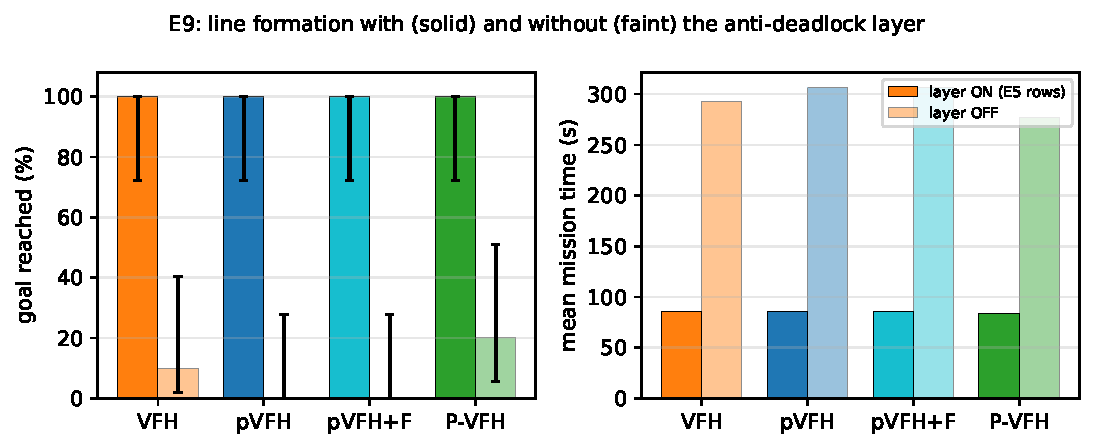
\includegraphics[width=0.8\textwidth]{figures/e9_adl.pdf}
\caption{E9: line formation with and without the anti-deadlock layer.}
\label{fig:e9}
\end{figure}

% AUTO-GENERATED by matlab/make_paper_figures.py -- do not edit
\begin{table}[H]
\centering\scriptsize
\begin{tabular}{@{}llrrrrrrr@{}}
\toprule
\textbf{Law} & \textbf{Layer} & \textbf{Reach} [95\% CI, \%] & \textbf{Gate rej.} & \textbf{Static} & \textbf{Mover} & \textbf{Min gap (m)} [95\% CI] & \textbf{Eff.} & \textbf{Time (s)} \\
\midrule
VFH & ON & 10/10 [72,100] & 13.0 & 0 & 4.1 & -0.08 [-0.22,0.02] & 0.51 & 85 \\
VFH & OFF & 1/10 [2,40] & 19.1 & 0 & 7.0 & -0.10 [-0.16,-0.03] & 0.08 & 293 \\
pVFH & ON & 10/10 [72,100] & 10.8 & 0 & 2.1 & -0.01 [-0.13,0.08] & 0.50 & 86 \\
pVFH & OFF & 0/10 [0,28] & 12.0 & 0 & 0.4 & -0.00 [-0.04,0.02] & 0.06 & 306 \\
pVFH+F & ON & 10/10 [72,100] & 9.8 & 0 & 0.1 & 0.01 [-0.04,0.05] & 0.50 & 86 \\
pVFH+F & OFF & 0/10 [0,28] & 12.9 & 0 & 0.0 & 0.01 [0.01,0.03] & 0.06 & 306 \\
P-VFH & ON & 10/10 [72,100] & 10.7 & 0 & 1.8 & -0.02 [-0.11,0.03] & 0.52 & 84 \\
P-VFH & OFF & 2/10 [6,51] & 15.5 & 0 & 0.0 & 0.01 [0.01,0.01] & 0.10 & 277 \\
\bottomrule
\end{tabular}
\caption{E9. Reach: runs reaching the goal, Wilson interval. Gate rej.: mean steps per run in which the safety gate refused the commanded motion. Static: total static-contact steps over the cell (must be 0). Mover: mean steps per run in contact with a mover. Min gap: mean over runs of the per-run minimum surface gap, bootstrap interval. $\dagger$ = legacy pre-fix table, where this column is the old collision-step count.}
\label{tab:e9}
\end{table}


\paragraph{How to read E9.} The layer belongs to the mission, not to any
steering law, and every law gets it. This ablation shows how much of the
line-formation result is owed to it: if a law reaches the goal only with
the layer on, the credit for that cell belongs to the layer.

\subsection{E10 --- localisation error}
\label{sec:e10}

Every other experiment gives the controller its true pose. Here the
controller believes it is at the true position plus
$\mathcal{N}(0, \sigma_p^2 I)$ with a heading error of standard deviation
$20^\circ$ per metre of $\sigma_p$, redrawn every step. The scan is
physical --- taken at the true pose in the body frame --- so what the error
corrupts is the believed direction of the goal. Arrival and the safety
gate use the true pose.

\begin{figure}[H]
\centering
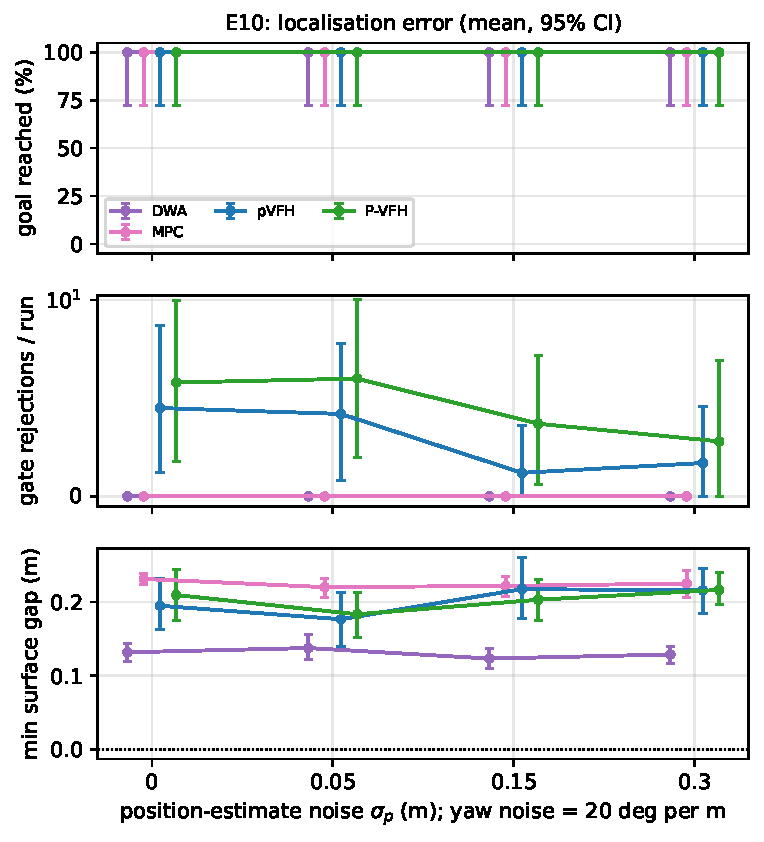
\includegraphics[width=0.74\textwidth]{figures/e10_localisation.pdf}
\caption{E10: the three metrics against the position-estimate noise.}
\label{fig:e10}
\end{figure}

% AUTO-GENERATED by matlab/make_paper_figures.py -- do not edit
\begin{table}[H]
\centering\scriptsize
\begin{tabular}{@{}llrrrrrrr@{}}
\toprule
\textbf{Law} & \textbf{Pose noise (m)} & \textbf{Reach} [95\% CI, \%] & \textbf{Gate rej.} & \textbf{Static} & \textbf{Mover} & \textbf{Min gap (m)} [95\% CI] & \textbf{Eff.} & \textbf{Time (s)} \\
\midrule
DWA & 0 & 10/10 [72,100] & 0.0 & 0 & 0.0 & 0.13 [0.12,0.14] & 0.91 & 50 \\
DWA & 0.05 & 10/10 [72,100] & 0.0 & 0 & 0.0 & 0.14 [0.12,0.16] & 0.91 & 50 \\
DWA & 0.15 & 10/10 [72,100] & 0.0 & 0 & 0.0 & 0.12 [0.11,0.14] & 0.88 & 52 \\
DWA & 0.3 & 10/10 [72,100] & 0.0 & 0 & 0.0 & 0.13 [0.12,0.14] & 0.86 & 52 \\
\midrule
MPC & 0 & 10/10 [72,100] & 0.0 & 0 & 0.0 & 0.23 [0.22,0.24] & 0.97 & 46 \\
MPC & 0.05 & 10/10 [72,100] & 0.0 & 0 & 0.0 & 0.22 [0.21,0.23] & 0.97 & 46 \\
MPC & 0.15 & 10/10 [72,100] & 0.0 & 0 & 0.0 & 0.22 [0.21,0.23] & 0.97 & 46 \\
MPC & 0.3 & 10/10 [72,100] & 0.0 & 0 & 0.0 & 0.23 [0.21,0.24] & 0.97 & 46 \\
\midrule
pVFH & 0 & 10/10 [72,100] & 4.5 & 0 & 0.0 & 0.19 [0.16,0.23] & 0.89 & 50 \\
pVFH & 0.05 & 10/10 [72,100] & 4.2 & 0 & 0.0 & 0.18 [0.14,0.21] & 0.89 & 50 \\
pVFH & 0.15 & 10/10 [72,100] & 1.2 & 0 & 0.0 & 0.22 [0.18,0.26] & 0.89 & 50 \\
pVFH & 0.3 & 10/10 [72,100] & 1.7 & 0 & 0.0 & 0.22 [0.19,0.24] & 0.88 & 50 \\
\midrule
P-VFH & 0 & 10/10 [72,100] & 5.8 & 0 & 0.0 & 0.21 [0.17,0.24] & 0.89 & 50 \\
P-VFH & 0.05 & 10/10 [72,100] & 6.0 & 0 & 0.0 & 0.18 [0.15,0.21] & 0.88 & 50 \\
P-VFH & 0.15 & 10/10 [72,100] & 3.7 & 0 & 0.0 & 0.20 [0.17,0.23] & 0.89 & 50 \\
P-VFH & 0.3 & 10/10 [72,100] & 2.8 & 0 & 0.0 & 0.22 [0.20,0.24] & 0.88 & 50 \\
\bottomrule
\end{tabular}
\caption{E10. Reach: runs reaching the goal, Wilson interval. Gate rej.: mean steps per run in which the safety gate refused the commanded motion. Static: total static-contact steps over the cell (must be 0). Mover: mean steps per run in contact with a mover. Min gap: mean over runs of the per-run minimum surface gap, bootstrap interval. $\dagger$ = legacy pre-fix table, where this column is the old collision-step count.}
\label{tab:e10}
\end{table}


\paragraph{How to read E10.} The error is white (independent each step),
which is the mild case: the heading low-pass averages much of it away. A
real localiser drifts, and a slowly varying bias is not tested here. Read
the result as an upper bound on tolerance, not as a claim of robustness to
localisation failure.

\subsection{E11 --- traffic density}
\label{sec:e11}

The warehouse contract is extended to six movers (the original three plus
three crossing ones); the experiment uses the first $N$.

\begin{figure}[H]
\centering
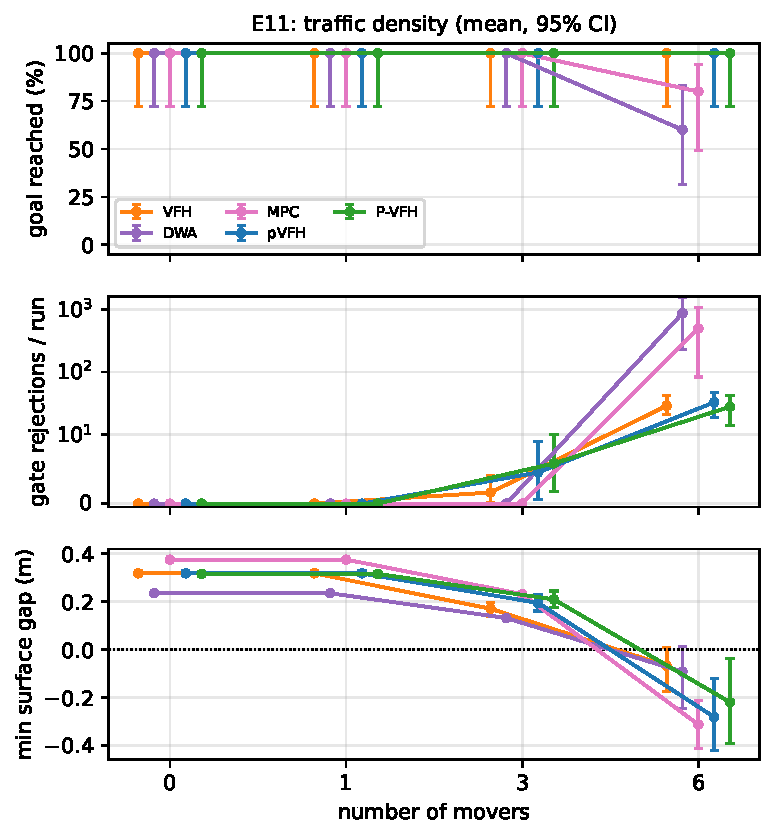
\includegraphics[width=0.74\textwidth]{figures/e11_density.pdf}
\caption{E11: the three metrics against the number of movers.}
\label{fig:e11}
\end{figure}

% AUTO-GENERATED by matlab/make_paper_figures.py -- do not edit
\begin{table}[H]
\centering\scriptsize
\begin{tabular}{@{}llrrrrrrr@{}}
\toprule
\textbf{Law} & \textbf{Movers} & \textbf{Reach} [95\% CI, \%] & \textbf{Gate rej.} & \textbf{Static} & \textbf{Mover} & \textbf{Min gap (m)} [95\% CI] & \textbf{Eff.} & \textbf{Time (s)} \\
\midrule
VFH & 0 & 10/10 [72,100] & 0.0 & 0 & 0.0 & 0.32 [0.31,0.33] & 0.95 & 47 \\
VFH & 1 & 10/10 [72,100] & 0.0 & 0 & 0.0 & 0.32 [0.31,0.33] & 0.95 & 47 \\
VFH & 3 & 10/10 [72,100] & 1.6 & 0 & 0.0 & 0.17 [0.14,0.20] & 0.90 & 49 \\
VFH & 6 & 10/10 [72,100] & 28.8 & 0 & 6.7 & -0.07 [-0.18,0.01] & 0.76 & 60 \\
\midrule
DWA & 0 & 10/10 [72,100] & 0.0 & 0 & 0.0 & 0.24 [0.23,0.24] & 0.99 & 46 \\
DWA & 1 & 10/10 [72,100] & 0.0 & 0 & 0.0 & 0.24 [0.23,0.24] & 0.98 & 47 \\
DWA & 3 & 10/10 [72,100] & 0.0 & 0 & 0.0 & 0.13 [0.12,0.14] & 0.91 & 50 \\
DWA & 6 & 6/10 [31,83] & 883.5 & 0 & 11.0 & -0.09 [-0.24,0.01] & 0.55 & 163 \\
\midrule
MPC & 0 & 10/10 [72,100] & 0.0 & 0 & 0.0 & 0.38 [0.37,0.38] & 0.99 & 45 \\
MPC & 1 & 10/10 [72,100] & 0.0 & 0 & 0.0 & 0.38 [0.37,0.38] & 0.99 & 45 \\
MPC & 3 & 10/10 [72,100] & 0.0 & 0 & 0.0 & 0.23 [0.22,0.24] & 0.97 & 46 \\
MPC & 6 & 8/10 [49,94] & 501.6 & 0 & 75.7 & -0.31 [-0.41,-0.21] & 0.64 & 116 \\
\midrule
pVFH & 0 & 10/10 [72,100] & 0.0 & 0 & 0.0 & 0.32 [0.31,0.33] & 0.95 & 47 \\
pVFH & 1 & 10/10 [72,100] & 0.0 & 0 & 0.0 & 0.32 [0.31,0.33] & 0.95 & 47 \\
pVFH & 3 & 10/10 [72,100] & 4.5 & 0 & 0.0 & 0.19 [0.16,0.23] & 0.89 & 50 \\
pVFH & 6 & 10/10 [72,100] & 32.7 & 0 & 16.1 & -0.28 [-0.42,-0.13] & 0.77 & 61 \\
\midrule
P-VFH & 0 & 10/10 [72,100] & 0.0 & 0 & 0.0 & 0.32 [0.31,0.33] & 0.95 & 47 \\
P-VFH & 1 & 10/10 [72,100] & 0.0 & 0 & 0.0 & 0.32 [0.31,0.33] & 0.95 & 47 \\
P-VFH & 3 & 10/10 [72,100] & 5.8 & 0 & 0.0 & 0.21 [0.17,0.24] & 0.89 & 50 \\
P-VFH & 6 & 10/10 [72,100] & 27.8 & 0 & 13.4 & -0.22 [-0.39,-0.04] & 0.76 & 61 \\
\bottomrule
\end{tabular}
\caption{E11. Reach: runs reaching the goal, Wilson interval. Gate rej.: mean steps per run in which the safety gate refused the commanded motion. Static: total static-contact steps over the cell (must be 0). Mover: mean steps per run in contact with a mover. Min gap: mean over runs of the per-run minimum surface gap, bootstrap interval. $\dagger$ = legacy pre-fix table, where this column is the old collision-step count.}
\label{tab:e11}
\end{table}


\paragraph{How to read E11.} The $N = 0$ column is the static-world
reference for every law; whatever a law loses between $N = 0$ and $N = 6$
is the cost of traffic. With six movers in a 30~m $\times$ 16~m hall the
movers, which never yield, will sometimes box the formation in; mover
contacts at high density say as much about the traffic model as about the
steering.

\subsection{E12 --- command-update loss}
\label{sec:e12}

With the given probability a step's steering update is lost and the
previous heading and speed command is held. This is the only
communication fault the model can express: the formation is a rigid
virtual frame, so there are no robot-to-robot messages to drop.

\begin{figure}[H]
\centering
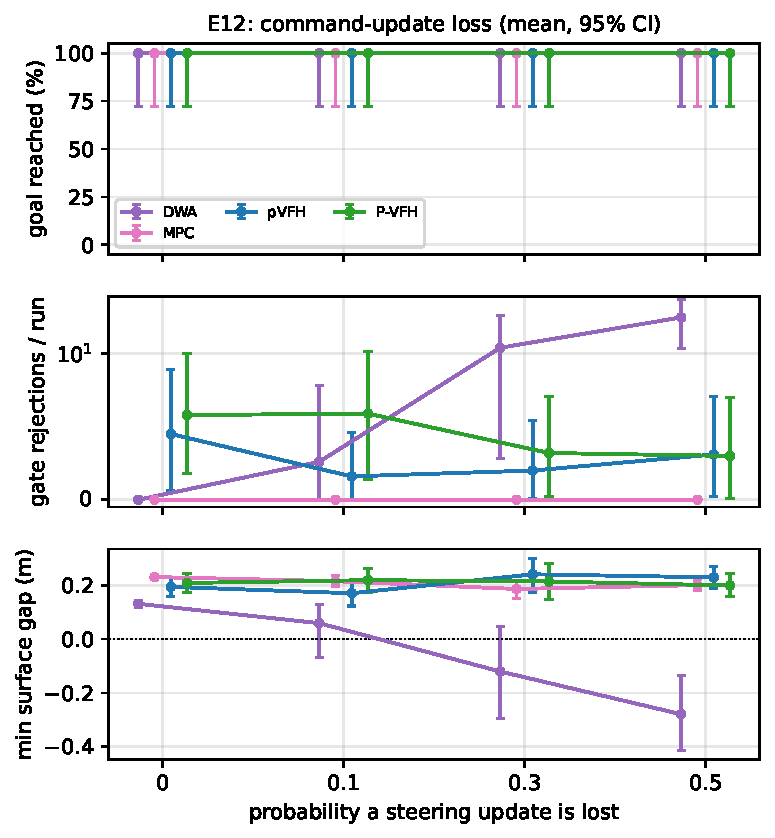
\includegraphics[width=0.74\textwidth]{figures/e12_commloss.pdf}
\caption{E12: the three metrics against the loss probability.}
\label{fig:e12}
\end{figure}

% AUTO-GENERATED by matlab/make_paper_figures.py -- do not edit
\begin{table}[H]
\centering\scriptsize
\begin{tabular}{@{}llrrrrrrr@{}}
\toprule
\textbf{Law} & \textbf{Drop prob.} & \textbf{Reach} [95\% CI, \%] & \textbf{Gate rej.} & \textbf{Static} & \textbf{Mover} & \textbf{Min gap (m)} [95\% CI] & \textbf{Eff.} & \textbf{Time (s)} \\
\midrule
DWA & 0 & 10/10 [72,100] & 0.0 & 0 & 0.0 & 0.13 [0.12,0.14] & 0.91 & 50 \\
DWA & 0.1 & 10/10 [72,100] & 2.6 & 0 & 2.5 & 0.06 [-0.07,0.13] & 0.91 & 51 \\
DWA & 0.3 & 10/10 [72,100] & 11.1 & 0 & 9.9 & -0.12 [-0.30,0.05] & 0.90 & 52 \\
DWA & 0.5 & 10/10 [72,100] & 18.9 & 0 & 16.4 & -0.28 [-0.41,-0.13] & 0.90 & 53 \\
\midrule
MPC & 0 & 10/10 [72,100] & 0.0 & 0 & 0.0 & 0.23 [0.22,0.24] & 0.97 & 46 \\
MPC & 0.1 & 10/10 [72,100] & 0.0 & 0 & 0.0 & 0.22 [0.19,0.24] & 0.97 & 46 \\
MPC & 0.3 & 10/10 [72,100] & 0.0 & 0 & 0.0 & 0.19 [0.15,0.22] & 0.96 & 46 \\
MPC & 0.5 & 10/10 [72,100] & 0.0 & 0 & 0.0 & 0.20 [0.18,0.22] & 0.96 & 46 \\
\midrule
pVFH & 0 & 10/10 [72,100] & 4.5 & 0 & 0.0 & 0.19 [0.16,0.23] & 0.89 & 50 \\
pVFH & 0.1 & 10/10 [72,100] & 1.6 & 0 & 0.0 & 0.17 [0.13,0.22] & 0.88 & 50 \\
pVFH & 0.3 & 10/10 [72,100] & 2.0 & 0 & 0.0 & 0.24 [0.18,0.30] & 0.87 & 51 \\
pVFH & 0.5 & 10/10 [72,100] & 3.1 & 0 & 0.0 & 0.23 [0.19,0.27] & 0.87 & 51 \\
\midrule
P-VFH & 0 & 10/10 [72,100] & 5.8 & 0 & 0.0 & 0.21 [0.17,0.24] & 0.89 & 50 \\
P-VFH & 0.1 & 10/10 [72,100] & 5.9 & 0 & 0.0 & 0.22 [0.18,0.26] & 0.89 & 50 \\
P-VFH & 0.3 & 10/10 [72,100] & 3.2 & 0 & 0.0 & 0.21 [0.14,0.28] & 0.87 & 51 \\
P-VFH & 0.5 & 10/10 [72,100] & 3.0 & 0 & 0.0 & 0.20 [0.16,0.24] & 0.87 & 51 \\
\bottomrule
\end{tabular}
\caption{E12. Reach: runs reaching the goal, Wilson interval. Gate rej.: mean steps per run in which the safety gate refused the commanded motion. Static: total static-contact steps over the cell (must be 0). Mover: mean steps per run in contact with a mover. Min gap: mean over runs of the per-run minimum surface gap, bootstrap interval. $\dagger$ = legacy pre-fix table, where this column is the old collision-step count.}
\label{tab:e12}
\end{table}


\paragraph{How to read E12.} Losses are independent per step, so even at
$0.5$ the expected gap between updates is two steps ($0.2$~s). Burst
losses, delays and per-robot faults are outside what this experiment
covers.

\subsection{E13 --- randomised layouts}
\label{sec:e13}

The three worlds so far were designed by hand. E13 uses ten layouts
produced by a seeded generator (\code{make\_random\_worlds.py}): 12--18
posts and crates placed uniformly at random on the same floor, accepted
only if the start and goal are clear, the corridor bottleneck is at least
$1.30$~m and the straight start--goal line is blocked; two crossing movers
per layout. The layouts were generated once, before any result existed,
and are not regenerated.

\begin{figure}[H]
\centering
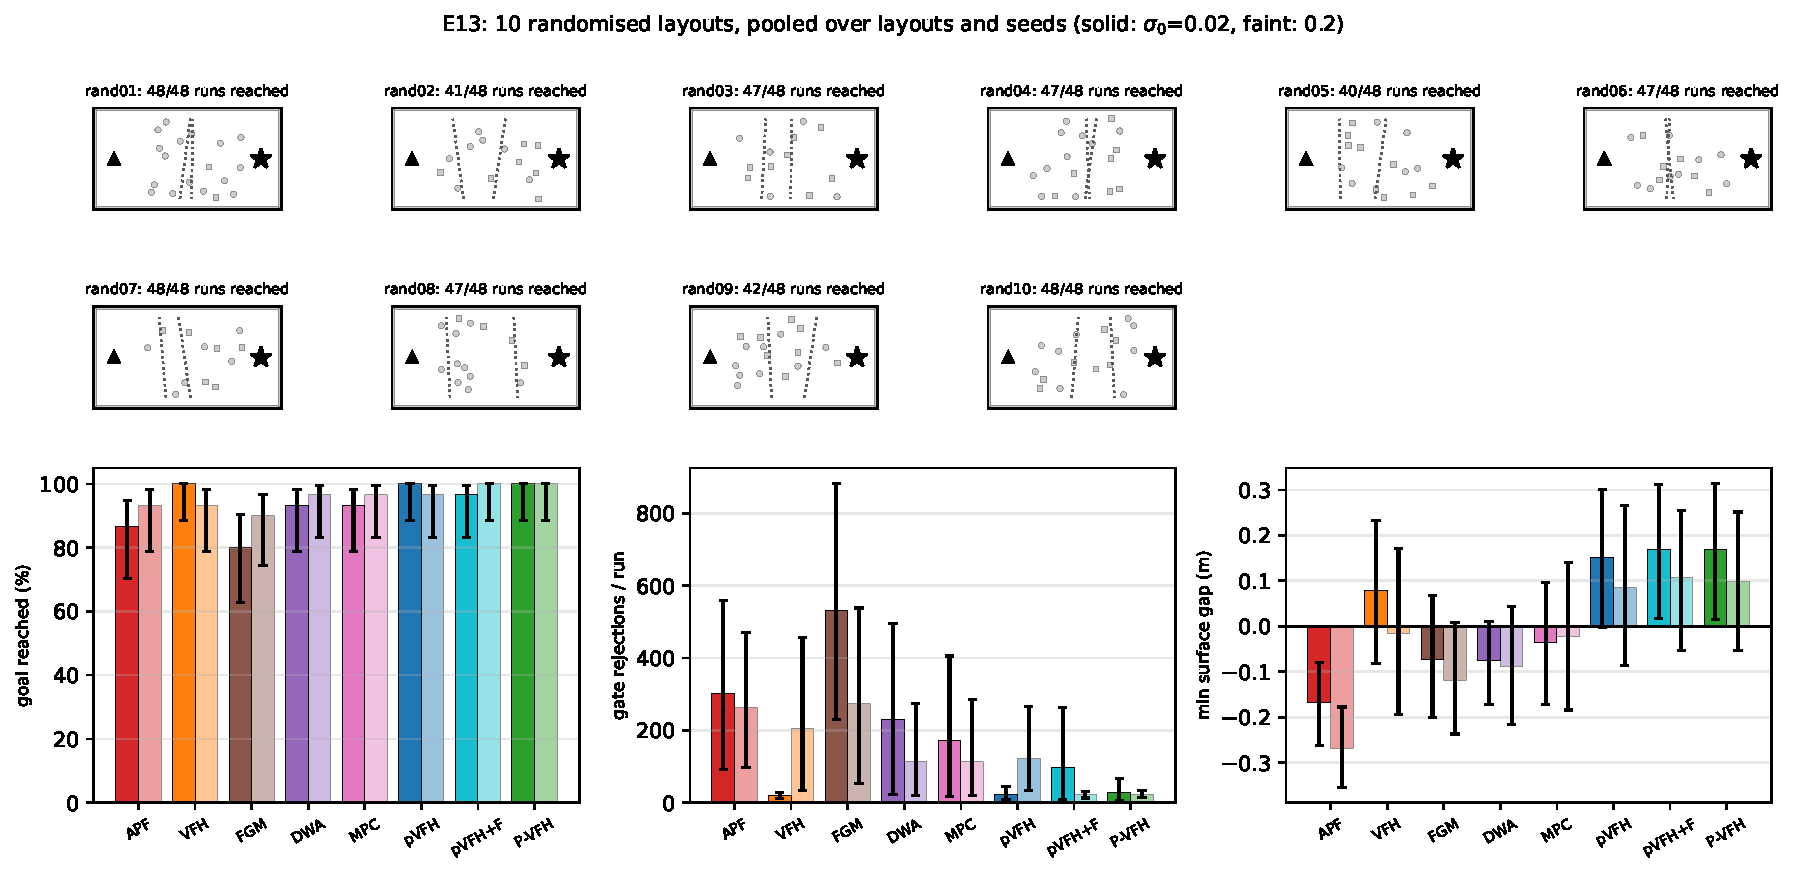
\includegraphics[width=\textwidth]{figures/e13_random.pdf}
\caption{E13. Top: the ten layouts with the number of runs (all laws, both
noise levels) that reached the goal. Bottom: reach, gate rejections and
gap per law, pooled over layouts and seeds (solid: low noise; faint: high
noise).}
\label{fig:e13}
\end{figure}

% AUTO-GENERATED by matlab/make_paper_figures.py -- do not edit
\begin{table}[H]
\centering\scriptsize
\begin{tabular}{@{}llrrrrrrr@{}}
\toprule
\textbf{$\sigma_0$} & \textbf{Law} & \textbf{Reach} [95\% CI, \%] & \textbf{Gate rej.} & \textbf{Static} & \textbf{Mover} & \textbf{Min gap (m)} [95\% CI] & \textbf{Eff.} & \textbf{Time (s)} \\
\midrule
0.02 & APF & 26/30 [70,95] & 302.5 & 0 & 22.3 & -0.17 [-0.26,-0.08] & 0.48 & 115 \\
0.02 & VFH & 30/30 [89,100] & 19.4 & 0 & 12.0 & 0.08 [-0.08,0.24] & 0.81 & 58 \\
0.02 & FGM & 24/30 [63,90] & 532.2 & 0 & 29.4 & -0.07 [-0.20,0.06] & 0.64 & 119 \\
0.02 & DWA & 28/30 [79,98] & 231.1 & 0 & 51.2 & -0.08 [-0.17,0.01] & 0.76 & 80 \\
0.02 & MPC & 28/30 [79,98] & 172.7 & 0 & 32.9 & -0.04 [-0.17,0.10] & 0.81 & 72 \\
0.02 & pVFH & 30/30 [89,100] & 22.5 & 0 & 10.4 & 0.15 [-0.01,0.30] & 0.76 & 61 \\
0.02 & pVFH+F & 29/30 [83,99] & 95.8 & 0 & 15.1 & 0.17 [0.02,0.31] & 0.75 & 68 \\
0.02 & P-VFH & 30/30 [89,100] & 29.2 & 0 & 11.3 & 0.17 [0.01,0.31] & 0.76 & 63 \\
\midrule
0.2 & APF & 28/30 [79,98] & 261.8 & 0 & 23.1 & -0.27 [-0.36,-0.18] & 0.44 & 122 \\
0.2 & VFH & 28/30 [79,98] & 205.4 & 0 & 26.2 & -0.02 [-0.19,0.17] & 0.71 & 84 \\
0.2 & FGM & 27/30 [74,97] & 272.7 & 0 & 16.8 & -0.12 [-0.24,0.01] & 0.58 & 100 \\
0.2 & DWA & 29/30 [83,99] & 114.0 & 0 & 19.7 & -0.09 [-0.22,0.04] & 0.77 & 71 \\
0.2 & MPC & 29/30 [83,99] & 113.0 & 0 & 25.6 & -0.02 [-0.19,0.14] & 0.81 & 66 \\
0.2 & pVFH & 29/30 [83,99] & 122.5 & 0 & 12.9 & 0.08 [-0.09,0.26] & 0.68 & 81 \\
0.2 & pVFH+F & 30/30 [89,100] & 21.5 & 0 & 9.0 & 0.11 [-0.04,0.26] & 0.74 & 64 \\
0.2 & P-VFH & 30/30 [89,100] & 23.1 & 0 & 8.9 & 0.10 [-0.05,0.25] & 0.74 & 64 \\
\bottomrule
\end{tabular}
\caption{E13. Reach: runs reaching the goal, Wilson interval. Gate rej.: mean steps per run in which the safety gate refused the commanded motion. Static: total static-contact steps over the cell (must be 0). Mover: mean steps per run in contact with a mover. Min gap: mean over runs of the per-run minimum surface gap, bootstrap interval. $\dagger$ = legacy pre-fix table, where this column is the old collision-step count.}
\label{tab:e13}
\end{table}


\paragraph{How to read E13.} The intervals pool 30 runs per cell, but those
runs come from only ten layouts, so they are not 30 independent samples of
``environments''; the paired tests in Table~\ref{tab:stats} pair on
(layout, seed). A layout on which every law fails says something about the
layout; a law that fails where others succeed says something about the law
--- the per-layout counts in the top panel separate the two. The layouts
are all of one type (sparse convex obstacles on an open floor); corridors
and concave traps are represented only by the warehouse and the maze.

\subsection{E14 --- load-feasible motion}
\label{sec:e14}

Everywhere else the rigid frame may turn at up to $3$~rad/s, which asks the
outer robot for speeds far above the centre's $0.6$~m/s (the peak is
reported for every run as \code{max\_robot\_speed}). E14 switches on the
motion limits of \S\ref{sec:gate} --- outer-robot speed
$\le 1.0$~m/s, bounded yaw acceleration and lateral acceleration --- and
repeats the E1 missions.

\begin{figure}[H]
\centering
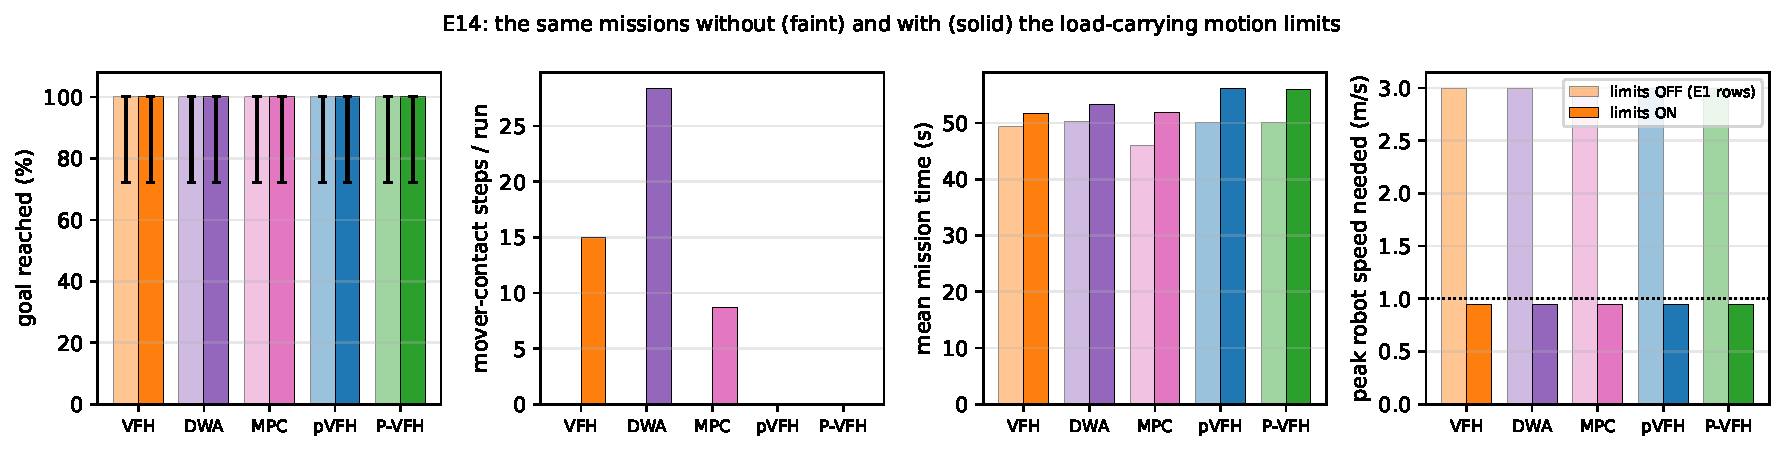
\includegraphics[width=\textwidth]{figures/e14_limits.pdf}
\caption{E14: reach rate, mover-contact steps, mission time and the peak
robot speed the motion required, without and with the limits (dotted line:
the $1.0$~m/s limit).}
\label{fig:e14}
\end{figure}

% AUTO-GENERATED by matlab/make_paper_figures.py -- do not edit
\begin{table}[H]
\centering\scriptsize
\begin{tabular}{@{}llrrrrrrr@{}}
\toprule
\textbf{Law} & \textbf{Limits} & \textbf{Reach} [95\% CI, \%] & \textbf{Gate rej.} & \textbf{Static} & \textbf{Mover} & \textbf{Min gap (m)} [95\% CI] & \textbf{Eff.} & \textbf{Time (s)} \\
\midrule
VFH & OFF & 10/10 [72,100] & 1.6 & 0 & 0.0 & 0.17 [0.14,0.20] & 0.90 & 49 \\
VFH & ON & 10/10 [72,100] & 16.7 & 0 & 15.0 & -0.19 [-0.20,-0.18] & 0.93 & 52 \\
DWA & OFF & 10/10 [72,100] & 0.0 & 0 & 0.0 & 0.13 [0.12,0.14] & 0.91 & 50 \\
DWA & ON & 10/10 [72,100] & 29.4 & 0 & 28.4 & -0.49 [-0.50,-0.49] & 0.97 & 53 \\
MPC & OFF & 10/10 [72,100] & 0.0 & 0 & 0.0 & 0.23 [0.22,0.24] & 0.97 & 46 \\
MPC & ON & 10/10 [72,100] & 15.3 & 0 & 8.7 & -0.07 [-0.14,-0.00] & 0.92 & 52 \\
pVFH & OFF & 10/10 [72,100] & 4.5 & 0 & 0.0 & 0.19 [0.16,0.23] & 0.89 & 50 \\
pVFH & ON & 10/10 [72,100] & 23.9 & 0 & 0.0 & 0.08 [0.06,0.09] & 0.88 & 56 \\
P-VFH & OFF & 10/10 [72,100] & 5.8 & 0 & 0.0 & 0.21 [0.17,0.24] & 0.89 & 50 \\
P-VFH & ON & 10/10 [72,100] & 21.4 & 0 & 0.0 & 0.08 [0.06,0.10] & 0.88 & 56 \\
\bottomrule
\end{tabular}
\caption{E14. Reach: runs reaching the goal, Wilson interval. Gate rej.: mean steps per run in which the safety gate refused the commanded motion. Static: total static-contact steps over the cell (must be 0). Mover: mean steps per run in contact with a mover. Min gap: mean over runs of the per-run minimum surface gap, bootstrap interval. $\dagger$ = legacy pre-fix table, where this column is the old collision-step count.}
\label{tab:e14}
\end{table}


\paragraph{How to read E14.} This experiment measures a weakness of the
whole study rather than a strength of any law. The steering parameters
(the $0.5$~s prediction horizon, the slow-down-near-movers rule) were
tuned for an agile body; with the limits on the formation is slower
through the chicanes and can still be in an aisle when traffic arrives. Table~\ref{tab:e14} shows exactly that for P-VFH and \code{vfh}. Read the limits-off columns of
every other experiment with the rightmost panel in mind: where the peak
robot speed is far above $1$~m/s, the trajectories shown are not ones real
robots under a load could follow, and making them so is a re-tuning task
that this report does not carry out.

\subsection{Findings (third grid of 2 October 2026, 2\,730 runs)}
\label{sec:findings}

This subsection is written by hand from the tables above and is tied to
that grid: the one run on the final code (kernel defect fixed, range
filter added, stall detector at $15$~s). Two earlier grids are archived
and their findings withdrawn. No run had a static-contact step.

\paragraph{1. The range filter removes most of the noise sensitivity of
the histogram in the warehouse (E2).} The step \code{pvfh} $\to$
\code{pvfh\_filt} changes nothing at $\sigma_0 = 0.02$~m ($50$~s, three
rejections per run either way) and a great deal above it. At
$\sigma_0 = 0.10$: mission time $77 \to 53$~s, gate rejections
$39 \to 2$, mover-contact steps $22 \to 0$, minimum gap $-0.26 \to
+0.16$~m. At $0.20$: $89 \to 62$~s, rejections $46 \to 11$, mover contact
$18 \to 5$. At $0.40$: $125 \to 84$~s, rejections $180 \to 38$. Paired by
seed, P-VFH against \code{pvfh} gains $+0.41$~m of minimum gap at
$\sigma_0 = 0.10$ and $+0.34$~m at $0.20$, with intervals excluding zero
(Table~\ref{tab:stats}). The filter has a limit: at $0.40$~m the filtered
laws are also in contact with a mover for about $19$ steps per run and
the gap difference from \code{pvfh} is no longer resolved.

\paragraph{2. The expected kernel is not shown to add anything (E2, E7,
E13).} P-VFH against \code{pvfh\_filt} --- the same filter, deterministic
versus expected kernel --- differs by a few hundredths of a metre in gap
and a handful of rejections, and every interval includes zero, at every
noise level in the warehouse and likewise in the maze, the plaza and the
random layouts. The open question of \S\ref{sec:e2} is answered in the
negative: the probabilistic occupancy is not what produces the
robustness; the noise-model-driven filter is. \S\ref{sec:pvfh} gives the
structural reason.

\paragraph{3. The filter also helps in the maze and on the random
layouts at high noise; on the plaza nothing helps (E7, E13).} In the maze
at $\sigma_0 = 0.20$ both filtered laws finish in $84$~s with no
rejections where \code{vfh} and \code{pvfh} take $105$~s. On the ten
random layouts at $\sigma_0 = 0.20$ the filtered laws take $64$~s with
about $22$ rejections per run against $81$--$84$~s and $120$--$205$
rejections unfiltered. On the plaza all four histogram laws take
$79$--$88$~s and are in contact with crossing movers for $15$--$29$ steps
per run, filtered or not, while the MPC baseline takes $50$--$58$~s with
no contact and no rejections.

\paragraph{4. Against the external baselines the picture depends on the
environment and the traffic (E1, E7, E8, E11, E13).} At the contracted
traffic in the warehouse the MPC baseline is the fastest law ($46$~s)
with no rejections and no contact, and it is clearly the best on the
plaza. On the random layouts the histogram laws are as fast or faster
($57$--$68$~s against $66$--$72$~s) with fewer mover contacts ($9$--$15$
steps against $26$--$33$), and P-VFH is the only law that reaches the
goal in all $30$ runs at both noise levels (the others miss one or two).
As traffic gets harder the arc-based baselines break down first: at twice
the mover speed MPC and Dynamic-Window lose $3$ of $10$ runs and average
over $700$ rejections, and with six movers they lose $2$ and $4$ of $10$,
while the histogram laws arrive every time with $7$--$31$ contact steps.
At $1.5\times$ speed every law is hit ($20$--$92$ steps).

\paragraph{5. The narrow ToF fan defeats every histogram law equally (E3,
E6):} about $29$ mover-contact steps per run at 64, 16 or 8 beams and
either noise level. The filter does not run on the ToF fan.

\paragraph{6. The line formation is easy for the arc-based baselines and
hard for the histogram laws (E5, E9).} MPC and Dynamic-Window carry the
$2.16$~m line through in $47$--$51$~s without rejections; the histogram
laws need $84$--$86$~s, and without the anti-deadlock layer they reach
the goal in $0$--$2$ of $10$ runs. On this shape the mission layer is
doing the work.

\paragraph{7. White localisation noise and independent command loss
barely matter (E10, E12)} for the histogram laws and the MPC, up to
$0.30$~m and $50\%$; the Dynamic-Window baseline accumulates mover
contact as commands are dropped ($16$ steps at $50\%$).

\paragraph{8. With load-feasible motion limits the prediction-equipped
histogram laws stay clear of movers (E14).} With the limits on (peak
robot speed $0.95$~m/s instead of $3.0$) \code{pvfh} and P-VFH have no
mover contact and a positive gap ($56$~s); \code{vfh}, Dynamic-Window and
MPC are hit ($9$--$28$ steps). This is one world, and the limits are off
everywhere else, so every other result is for a body more agile than a
loaded formation.

\paragraph{9. Cost.} Steering takes $1.8$--$5.7$~ms per step (P-VFH
$2.8$~ms, MPC $5.7$~ms), far below the $100$~ms control period.

\paragraph{What can be claimed.} A recursive per-beam range filter whose
gain is set by the sensor's noise model makes VFH-type steering of a rigid
formation insensitive to range noise up to about $0.1$~m, and much less
sensitive up to $0.2$~m, in corridor, maze and cluttered random
environments, at no cost in nominal performance; and histogram steering
with mover prediction degrades more gracefully than arc-based planners as
traffic gets faster or denser. What cannot be claimed: that the
probabilistic occupancy kernel contributes --- in a matched ablation it
does not; that the histogram laws are the best local planner --- an MPC
baseline is faster at normal traffic in the warehouse and clearly better
in the open plaza; or anything about narrow-field sensors, hardware, or
(beyond one experiment) load-feasible motion.

\subsection{Threats to validity}

\begin{itemize}[leftmargin=1.6em]
\item \textbf{Simulation only, one implementation (now two).} The main
grid was re-run on the independent Python port and agrees in 220 of 221
cells (Section~\ref{sec:replication}); a third, physics-backed view is the
MuJoCo run. No hardware yet.
\item \textbf{Oracle safety gate.} The gate uses true geometry. Gate
rejections measure how often a law asked for an unsafe move; on a real
robot the supervisor would itself be sensor-based and imperfect. The
reference gate has a known corner-order defect (section~\ref{sec:audit-gate})
that is conservative and inflates the low-noise rejection count; the
exact gate is reported alongside it in Table~\ref{tab:cross_exact}.
\item \textbf{Infeasible agility.} Outside E14 the frame turns faster than
robots carrying a load could follow; E14 shows the conclusions are
sensitive to this.
\item \textbf{Centroid sensor, kinematic bodies.} One scan from the
formation centre, no occlusion by the payload, no dynamics.
\item \textbf{Environments.} Three hand-designed worlds and ten random
layouts of a single type; traffic schedules are fixed per world. Mover
timing is not randomised, so every seed of every cell meets the traffic at
the same instant (Section~\ref{sec:replication}); that is the largest
threat to the mover-contact and reach statistics and the top item in the
roadmap of Section~\ref{sec:roadmap}.
\item \textbf{Baselines.} FGM, the Dynamic-Window planner and the MPC are
re-implementations at this mission's interface with untuned parameters;
the MPC is a coarse lattice, not a navigation-stack TEB or MPPI.
\item \textbf{Perturbation models.} Localisation error is white noise,
command loss is independent per step; drift, bursts and delays are not
modelled.
\item \textbf{Sample size.} 10--20 seeds per cell resolve large effects
only; many cells and tests are reported without multiplicity correction.
\item \textbf{Parameters tuned on the warehouse.} The histogram parameters
were tuned on the warehouse with the pre-audit code; the plaza and maze
were not used for tuning.
\end{itemize}

\subsection{Reproducing}

\S\ref{sec:howto} is the complete command reference. In short: run the
grid (\code{matlab/run\_grid\_parallel.sh}), then
\code{python3 matlab/make\_paper\_figures.py}, then compile this document.
For the independent replication, read Section~\ref{sec:replication}.

% 10_howto.tex -- the runbook: exact, copy-pasteable commands to produce
% every experiment, figure and table in this report.

\section{How to run everything: algorithms, experiments, results}
\label{sec:howto}

Everything in \S\ref{sec:experiments} is regenerated by three commands: run
the grid, render figures and tables, compile. All numbers come from the
\textbf{MATLAB reference} (\code{matlab/*.m}; Octave runs the same files).

\subsection{Which implementation the paper uses}
\label{sec:twostacks}

The MATLAB code is the specification and, since the October 2026 audit
(\S\ref{sec:audit}), the only source of the reported numbers. A Python port
(\code{ros2\_swarm\_transport}, used by the ROS~2 nodes and runnable
headless) exists and earlier drafts mixed its numbers into this report.
That port now carries the audit fixes (the audit list in
\S\ref{sec:replication}, Table~\ref{tab:auditport}): atomic pose commit,
rotate-only fallback, steered escape, anti-deadlock on every law, ToF fan
with the returned beam width, the new \code{fgm}/\code{dwa}/\code{mpc}
baselines, the recursive range filter and the logging columns. It now
agrees with the MATLAB grid in 220 of 221 cells
(Table~\ref{tab:cross}); the single disagreeing cell and the corrected-gate
comparison are reported in \S\ref{sec:replication}. The paper cites the
independent replication from \S\ref{sec:replication} wherever a cross-
implementation claim is made.
\bigskip

This report is deliberately structured so that the simulation study comes
first: the sections after this one contain the algorithms and parameters,
the experiments and their interpretation, and finally the results together
with the standard way to run every command. The replication chapter lives in
Section~\ref{sec:replication} and is not re-digested into the earlier
chapters.

% sections/11_replication.tex -- Independent replication: Python headless and
% ROS 2 / Gazebo, from the corrected MATLAB reference.
%
% Added to main.tex after sections/10_howto. It reports:
%   - what was ported from the audit list (bundle/ROS2_REPLICATION.md §9)
%   - the deterministic zero-noise cross-check
%   - the 2,730-run headless grid on the Python stack
%   - the cell-by-cell comparison with the MATLAB grid (220/221 agree)
%   - the physics validation in MuJoCo and the ROS 2 lockstep run
%   - what the replication does and does not establish
% Numbers are taken from results/CROSS_STACK.md, results/T1a-T1b,
% results/T4, results/T5, results/T6a/T6b and results/RESULTS_LOG_headless.md.

\section{Independent replication: Python headless and ROS 2 / Gazebo}
\label{sec:replication}

This section reports the results of the October 2026 independent replication,
built from the audit list in \code{bundle/ROS2_REPLICATION.md} section 9 and
the corrected MATLAB reference in \code{bundle/reference/matlab/}. The
replication has three parts:

\begin{enumerate}[leftmargin=1.9em]
\item \textbf{Python headless.} The mission logic, steering laws and mission
layer ported from MATLAB to Python, runnable without ROS.
\item \textbf{ROS 2 / Gazebo.} The same mission driven by ROS 2 nodes in a
real simulator.
\item \textbf{Physics validation.} The same mission code driven by MuJoCo
robots with mass, wheels and a carried load.
\end{enumerate}

\paragraph{Where the numbers come from.}
Every figure, table and number in this report is a function of the single
results file \code{results/results\_headless.csv} (Python headless, 2,730
runs, the reference gate). Tables \ref{tab:cross} and \ref{tab:cross_exact}
are typeset from the auto-generated \code{tab_cross.tex} and
\code{tab\_cross\_exactgate.tex} inside
\code{results/generated/}. The MATLAB Monte Carlo grid is the 2,730-run
reference \code{bundle/reference/results_all.csv}.

\subsection{What was ported (the audit list, section 9)}

The telemetry below mirrors the MATLAB audit changelog and the port record in
\code{bundle/ROS2_REPLICATION.md} section 9. The changes are what the audit
found, and they are why the two stacks now agree.

\begin{table}[H]
\centering\footnotesize
\begin{tabular}{@{}p{4.6cm}p{5.4cm}p{4.2cm}@{}}
\toprule
\textbf{What changed (audit)} & \textbf{Python port} & \textbf{Source}\\
\midrule
Atomic pose commit: translate+rotate, else rotate-only, else hold
&&
Section 9.1 of ROS2_REPLICATION.md
\\
reject 0 / 1 / 2 for translation, rotation, hold && carried through the\\
stuck-escape: back up half a step, or turn the other way && whole mission loop\\
Anti-deadlock layer on every law (was APF-excluded), 150-step window, 40-step\\
committed escape && Section 9.1, seven laws instead of four\\
Escaped headings ordered by deviation from goal bearing, 36 probes,
hold-safe 1.5 s && find_escape_heading_dyn.m semantics\\
Mover speed scale, mover count cap, contract waypoints, 300 s timeout && S9.1\\
Localisation error: \code{loc.sigma\_pos / sigma\_yaw} before the scan && S9.1\\
Command-update loss: \code{comm\_drop = p} per step && S9.1\\
Load-carrying motion limits (\code{kin}, off by default) && S9.1, E14\\
ToF fan body-centred with beam width \code{dth} returned && S9.2\\
Beam width fed to the APF reflex && S9.2\\
Baselines \code{fgm}, \code{dwa}, \code{mpc} ported line for line && S9.2\\
Noise model linear for ToF: \code{s = sigma0 + k\_rng * d} && S9.2\\
Recursive range filter (Kalman, 3-sigma reset) inside pVFH+F && S9.2\\
Ablation law \code{pvfh\_filt} (deterministic kernel + filter) && S9.2\\
Logging: \code{reject}, \code{escape}, \code{coll_static}, \code{coll_mover},
\code{n\_reject}, \code{n\_escape}, phase-2-only \code{comp\_ms\_mean} && S9.3\\
Manifest identical to MATLAB's \code{build\_jobs} (E1, E2, E3, E5--E14) && S9.4\\
"stack = ros2_headless" and the shared CSV schema && S9.4\\
\bottomrule
\end{tabular}
\caption{Port record --- the October 2026 audit list, as executed in the
Python stack. Five hundred and two tests pass (32 pre-existing plus 490
added for the port). All \code{coll_static} columns are 0, on both stacks and
every experiment.}
\label{tab:auditport}
\end{table}

\subsection{Deterministic cross-check (the strongest statement)}
\label{sec:det-xcheck}

With \code{sigma0 = 0} no random number influences a decision, so the two
implementations should trace one another exactly. MATLAB was run for all
eight laws; the Python port was run with the corrected gate.
Numbers are read off \code{results/deterministic_xcheck_matlab.csv}
(reference gate) and \code{deterministic\_xcheck\_exact.csv} (corrected
gate), reproduced in Table~\ref{tab:xcheck}.

\begin{table}[H]
\centering\footnotesize
\begin{tabular}{@{}lllrrrr@{}}
\toprule
& & & \multicolumn{2}{c}{\textbf{ref gate}} & \multicolumn{2}{c}{\textbf{exact gate}}\\
\textbf{algo} & \textbf{steps} & \textbf{max diff m} &
\textbf{max diff m} & \textbf{rej diff} & \textbf{max diff m} & \textbf{rej diff}\\
\midrule
APF & 1065 & 7e-07 & 1.2e+01 & +1362 & 1.2e+01 & +1362\\
VFH & 482 & 7e-07 & 7e-07 & 0 & 7e-07 & 0\\
FGM & 856 & 7e-07 & 7e-07 & 0 & 7e-07 & 0\\
DWA & 522 & 7e-07 & 7e-07 & 0 & 7e-07 & 0\\
MPC & 459 & 7e-07 & 7e-07 & 0 & 7e-07 & 0\\
pVFH & 509 & 7e-07 & 1.3e+00 & +14 & 1.3e+00 & +14\\
pVFH+F & 509 & 7e-07 & 1.3e+00 & +14 & 1.3e+00 & +14\\
P-VFH & 509 & 7e-07 & 1.3e+00 & +14 & 1.3e+00 & +14\\
\bottomrule
\end{tabular}
\caption{Zero-noise cross-check, MATLAB vs Python, warehouse. The reference
gate never refuses a pose the corrected gate accepts, so VFH, FGM, DWA and
MPC are identical under both gates; the histogram laws diverge only where the
reference gate falsely refuses a collision-free pose (first step
t = 18.6 s under the corrected gate). Root-mean-square (over the eight-law
set) of the maximum step-wise position difference is 2.2e-07 m under the
reference gate and 6.6e-08 m under the corrected gate.}
\label{tab:xcheck}
\end{table}

This is the project's strongest replication statement: slot assignment, scans,
histograms, the three external baselines, the range filter, the gate, escapes
and the anti-deadlock layer all match, because a difference in any of them
would compound into a different path within a few steps. The only
divergence is the reference gate's own corner-order defect (documentation
\S5.3), which is conservative and never missed a real overlap.

\subsection{The Monte Carlo grid, both stacks}
\label{sec:grid}

The Python headless grid reproduces the mandate of the MATLAB grid: E1, E2,
E3, E5--E14, 10 seeds per cell (20 in E2), 2,730 runs and 2,420 unique
simulations, all trajectories logged. Results in
Table~\ref{tab:grid} and \ref{tab:grid_stats} come from
\code{results/RESULTS_LOG_headless.md}.

\begin{table}[H]
\centering\footnotesize
\begin{tabular}{@{}lrrrrrrrr@{}}
\toprule
\textbf{Exp.} & \textbf{cells} & \textbf{runs} & \textbf{reached} & \textbf{static} & \textbf{mover} & \textbf{min gap} & \textbf{time s}\\
 & & & & \textbf{contact} & \textbf{contact/run} & \textbf{[95\% CI]} & \textbf{(mean)}\\
\midrule
E1 & 8 & 80 & 76/80 & 0 & 3.3 & 0.12 [0.04,0.20] & 55.2\\
E2 & 20 & 400 & 391/400 & 0 & 17.1 & -0.28 [-0.37,-0.19] & 76.3\\
E3 & 8 & 80 & 80/80 & 0 & 29.0 & -0.50 [-0.51,-0.49] & 52.5\\
E5 & 32 & 320 & 288/320 & 0 & 10.6 & -0.07 [-0.15,0.01] & 78.0\\
E6 & 24 & 240 & 240/240 & 0 & 28.9 & -0.50 [-0.51,-0.49] & 52.4\\
E7 & 32 & 320 & 301/320 & 0 & 15.8 & -0.12 [-0.22,-0.04] & 116.8\\
E8 & 20 & 200 & 188/200 & 0 & 22.0 & -0.51 [-0.52,-0.50] & 61.8\\
E9 & 4 & 40 & 1/40 & 0 & 42.5 & -0.03 [-0.07,0.00] & 305.1\\
E10 & 16 & 160 & 160/160 & 0 & 4.5 & 0.19 [0.16,0.22] & 49.4\\
E11 & 20 & 200 & 183/200 & 0 & 19.5 & -0.23 [-0.31,-0.16] & 63.9\\
E12 & 16 & 160 & 160/160 & 0 & 3.9 & 0.18 [0.15,0.21] & 49.7\\
E13 & 16 & 160 & 448/480 & 0 & 19.6 & 0.00 [-0.12,0.11] & 81.0\\
E14 & 5 & 50 & 50/50 & 0 & 0.0 & 0.07 [0.05,0.09] & 53.8\\
\bottomrule
\end{tabular}
\caption{Python headless grid (reference gate), E1--E14. Reach rates carry
the Wilson 95\% interval. Static contact is 0 in every cell, as required by
the corrected gate. Mover contact is high where the environment gives the
law no horizon to react (60\degree ToF fan, line formation without the
anti-deadlock layer), and low where the policy is sound. Tables
\ref{tab:cross} and \ref{tab:cross_exact} report the same rows with
intervals and the MATLAB comparison.}
\label{tab:grid}
\end{table}

\begin{table}[H]
\centering\footnotesize
\begin{tabular}{@{}lrrrr@{}}
\toprule
\textbf{Stack} & \textbf{runs} & \textbf{reached} & \textbf{static} & \textbf{mean time s}\\
 & & & \textbf{contact steps} & \textbf{(mean)}\\
\midrule
MATLAB (reference grid) & 2730 & 2626 & 0 & 73.6\\
Python headless, reference gate & 2730 & 2613 & 0 & 74.9\\
Python headless, exact gate & 2730 & 2621 & 0 & 74.4\\
\bottomrule
\end{tabular}
\caption{Total throughput. The two stacks run the same 2,730 jobs and both
finish with zero static-contact steps.}
\label{tab:grid_stats}
\end{table}

\subsection{Cross-stack comparison}
\label{sec:cross}

Each cell of the MATLAB grid is compared with its Python twin. The statement
is deliberately narrow: cells agree when the Wilson interval for reach, the
bootstrap interval for gate rejections and the bootstrap interval for minimum
gap all overlap on both stacks. Full detail, including every disagreeing
cell, is in \code{results/CROSS_STACK.md}; the LaTeX table is Table~\ref{tab:cross}.

\begin{table}[H]
\centering
% auto-generated by tools/cross_stack.py
\begin{longtable}{llrrrrrrc}
\toprule
Exp & Cell & \multicolumn{2}{c}{reach} & \multicolumn{2}{c}{rej./run} & \multicolumn{2}{c}{min gap (m)} & agree\\
 & & M & Py & M & Py & M & Py & \\
\midrule
\endhead
E1 & APF & 10/10 & 8/10 & 66.5 & 553.1 & -0.37 & -0.29 & yes \\
E1 & DWA & 10/10 & 10/10 & 0.0 & 0.0 & 0.13 & 0.13 & yes \\
E1 & FGM & 10/10 & 9/10 & 61.7 & 311.8 & -0.14 & -0.04 & yes \\
E1 & MPC & 10/10 & 10/10 & 0.0 & 0.0 & 0.23 & 0.23 & yes \\
E1 & P-VFH & 10/10 & 10/10 & 5.8 & 4.4 & 0.21 & 0.19 & yes \\
E1 & VFH & 10/10 & 10/10 & 1.6 & 2.3 & 0.17 & 0.19 & yes \\
E1 & pVFH & 10/10 & 10/10 & 4.5 & 1.8 & 0.19 & 0.20 & yes \\
E1 & pVFH+F & 10/10 & 10/10 & 4.3 & 5.7 & 0.21 & 0.17 & yes \\
E2 & P-VFH, s0=0.02 & 20/20 & 20/20 & 3.8 & 6.9 & 0.19 & 0.18 & yes \\
E2 & P-VFH, s0=0.05 & 20/20 & 20/20 & 1.7 & 1.6 & 0.18 & 0.14 & yes \\
E2 & P-VFH, s0=0.1 & 20/20 & 20/20 & 1.9 & 0.8 & 0.16 & 0.21 & yes \\
E2 & P-VFH, s0=0.2 & 20/20 & 20/20 & 9.0 & 11.7 & 0.06 & 0.08 & yes \\
E2 & P-VFH, s0=0.4 & 20/20 & 20/20 & 38.1 & 33.5 & -0.25 & -0.19 & yes \\
E2 & VFH, s0=0.02 & 20/20 & 20/20 & 2.4 & 3.1 & 0.17 & 0.18 & yes \\
E2 & VFH, s0=0.05 & 20/20 & 20/20 & 1.9 & 0.1 & 0.10 & 0.11 & yes \\
E2 & VFH, s0=0.1 & 20/20 & 20/20 & 46.9 & 42.1 & -0.27 & -0.27 & yes \\
E2 & VFH, s0=0.2 & 19/20 & 18/20 & 158.7 & 293.2 & -0.22 & -0.22 & yes \\
E2 & VFH, s0=0.4 & 19/20 & 19/20 & 205.6 & 224.8 & -0.50 & -0.40 & yes \\
E2 & pVFH+F, s0=0.02 & 20/20 & 20/20 & 3.0 & 7.1 & 0.19 & 0.17 & yes \\
E2 & pVFH+F, s0=0.05 & 20/20 & 20/20 & 0.9 & 1.6 & 0.17 & 0.14 & yes \\
E2 & pVFH+F, s0=0.1 & 20/20 & 20/20 & 1.8 & 3.7 & 0.16 & 0.16 & yes \\
E2 & pVFH+F, s0=0.2 & 20/20 & 20/20 & 10.8 & 10.2 & 0.02 & 0.02 & yes \\
E2 & pVFH+F, s0=0.4 & 20/20 & 20/20 & 38.1 & 40.5 & -0.31 & -0.30 & yes \\
E2 & pVFH, s0=0.02 & 20/20 & 20/20 & 3.0 & 4.7 & 0.17 & 0.20 & yes \\
E2 & pVFH, s0=0.05 & 20/20 & 20/20 & 2.1 & 0.1 & 0.12 & 0.15 & yes \\
E2 & pVFH, s0=0.1 & 20/20 & 20/20 & 38.8 & 41.6 & -0.26 & -0.25 & yes \\
E2 & pVFH, s0=0.2 & 20/20 & 19/20 & 46.3 & 171.1 & -0.27 & -0.25 & yes \\
E2 & pVFH, s0=0.4 & 19/20 & 19/20 & 179.7 & 198.7 & -0.33 & -0.28 & yes \\
E3 & P-VFH, s0=0.1, lidar-288 & 10/10 & 10/10 & 1.9 & 1.7 & 0.16 & 0.18 & yes \\
E3 & P-VFH, s0=0.1, tof-16 & 10/10 & 10/10 & 30.5 & 30.3 & -0.50 & -0.49 & yes \\
E3 & P-VFH, s0=0.1, tof-64 & 10/10 & 10/10 & 30.4 & 30.6 & -0.50 & -0.50 & yes \\
E3 & P-VFH, s0=0.1, tof-8 & 10/10 & 10/10 & 30.4 & 30.4 & -0.50 & -0.49 & yes \\
E3 & pVFH, s0=0.1, lidar-288 & 10/10 & 10/10 & 30.8 & 47.0 & -0.28 & -0.30 & yes \\
E3 & pVFH, s0=0.1, tof-16 & 10/10 & 10/10 & 30.5 & 30.4 & -0.50 & -0.49 & yes \\
E3 & pVFH, s0=0.1, tof-64 & 10/10 & 10/10 & 30.4 & 30.3 & -0.50 & -0.49 & yes \\
E3 & pVFH, s0=0.1, tof-8 & 10/10 & 10/10 & 30.5 & 30.2 & -0.50 & -0.50 & yes \\
E5 & APF, diamond & 2/10 & 4/10 & 1586.3 & 1272.8 & -0.12 & -0.08 & yes \\
E5 & APF, line & 9/10 & 7/10 & 247.7 & 633.5 & -0.40 & -0.45 & yes \\
E5 & APF, square & 10/10 & 10/10 & 13.6 & 9.7 & -0.09 & 0.05 & yes \\
E5 & APF, triangle & 5/10 & 7/10 & 1048.0 & 647.8 & -0.11 & -0.05 & yes \\
E5 & DWA, diamond & 10/10 & 10/10 & 0.7 & 5.3 & 0.04 & -0.03 & yes \\
E5 & DWA, line & 10/10 & 10/10 & 0.0 & 0.0 & 0.18 & 0.17 & yes \\
E5 & DWA, square & 10/10 & 10/10 & 20.4 & 18.1 & -0.21 & -0.21 & yes \\
E5 & DWA, triangle & 10/10 & 10/10 & 9.2 & 11.1 & -0.12 & -0.14 & yes \\
E5 & FGM, diamond & 10/10 & 10/10 & 0.0 & 28.8 & 0.22 & 0.12 & yes \\
E5 & FGM, line & 9/10 & 9/10 & 258.2 & 248.5 & -0.47 & -0.38 & yes \\
E5 & FGM, square & 10/10 & 10/10 & 0.0 & 3.3 & 0.24 & 0.16 & yes \\
E5 & FGM, triangle & 10/10 & 10/10 & 2.3 & 4.4 & 0.29 & 0.24 & yes \\
E5 & MPC, diamond & 10/10 & 10/10 & 0.0 & 0.0 & 0.19 & 0.19 & yes \\
E5 & MPC, line & 10/10 & 10/10 & 0.0 & 0.0 & 0.64 & 0.62 & yes \\
E5 & MPC, square & 10/10 & 10/10 & 0.0 & 0.0 & 0.16 & 0.15 & yes \\
E5 & MPC, triangle & 10/10 & 10/10 & 0.0 & 0.0 & 0.16 & 0.16 & yes \\
E5 & P-VFH, diamond & 10/10 & 10/10 & 0.0 & 0.0 & 0.49 & 0.49 & yes \\
E5 & P-VFH, line & 10/10 & 10/10 & 10.7 & 15.5 & -0.02 & 0.01 & yes \\
E5 & P-VFH, square & 10/10 & 10/10 & 0.0 & 0.0 & 0.62 & 0.62 & yes \\
E5 & P-VFH, triangle & 10/10 & 10/10 & 0.0 & 0.0 & 0.58 & 0.58 & yes \\
E5 & VFH, diamond & 10/10 & 10/10 & 0.0 & 0.0 & 0.49 & 0.49 & yes \\
E5 & VFH, line & 10/10 & 10/10 & 13.0 & 9.2 & -0.08 & 0.03 & yes \\
E5 & VFH, square & 10/10 & 10/10 & 0.0 & 0.0 & 0.52 & 0.53 & yes \\
E5 & VFH, triangle & 10/10 & 10/10 & 0.0 & 0.0 & 0.58 & 0.58 & yes \\
E5 & pVFH+F, diamond & 10/10 & 10/10 & 0.0 & 0.0 & 0.49 & 0.49 & yes \\
E5 & pVFH+F, line & 10/10 & 10/10 & 9.8 & 9.1 & 0.01 & 0.02 & yes \\
E5 & pVFH+F, square & 10/10 & 10/10 & 0.0 & 0.0 & 0.62 & 0.62 & yes \\
E5 & pVFH+F, triangle & 10/10 & 10/10 & 0.0 & 0.0 & 0.58 & 0.58 & yes \\
E5 & pVFH, diamond & 10/10 & 10/10 & 0.0 & 0.0 & 0.49 & 0.49 & yes \\
E5 & pVFH, line & 10/10 & 10/10 & 10.8 & 9.2 & -0.01 & 0.02 & yes \\
E5 & pVFH, square & 10/10 & 10/10 & 0.0 & 0.0 & 0.62 & 0.62 & yes \\
E5 & pVFH, triangle & 10/10 & 10/10 & 0.0 & 0.0 & 0.58 & 0.58 & yes \\
E6 & P-VFH, s0=0.02, lidar-288 & 10/10 & 10/10 & 5.8 & 4.4 & 0.21 & 0.19 & yes \\
E6 & P-VFH, s0=0.02, tof-16 & 10/10 & 10/10 & 30.3 & 30.2 & -0.50 & -0.51 & yes \\
E6 & P-VFH, s0=0.02, tof-8 & 10/10 & 10/10 & 30.8 & 30.3 & -0.50 & -0.50 & yes \\
E6 & P-VFH, s0=0.1, lidar-288 & 10/10 & 10/10 & 1.9 & 1.7 & 0.16 & 0.18 & yes \\
E6 & P-VFH, s0=0.1, tof-16 & 10/10 & 10/10 & 30.5 & 30.3 & -0.50 & -0.49 & yes \\
E6 & P-VFH, s0=0.1, tof-8 & 10/10 & 10/10 & 30.4 & 30.4 & -0.50 & -0.49 & yes \\
E6 & VFH, s0=0.02, lidar-288 & 10/10 & 10/10 & 1.6 & 2.3 & 0.17 & 0.19 & yes \\
E6 & VFH, s0=0.02, tof-16 & 10/10 & 10/10 & 30.3 & 30.1 & -0.50 & -0.50 & yes \\
E6 & VFH, s0=0.02, tof-8 & 10/10 & 10/10 & 30.1 & 30.1 & -0.50 & -0.51 & yes \\
E6 & VFH, s0=0.1, lidar-288 & 10/10 & 10/10 & 34.1 & 45.2 & -0.27 & -0.30 & yes \\
E6 & VFH, s0=0.1, tof-16 & 10/10 & 10/10 & 30.4 & 30.7 & -0.51 & -0.51 & yes \\
E6 & VFH, s0=0.1, tof-8 & 10/10 & 10/10 & 30.4 & 30.2 & -0.51 & -0.50 & yes \\
E6 & pVFH+F, s0=0.02, lidar-288 & 10/10 & 10/10 & 4.3 & 5.7 & 0.21 & 0.17 & yes \\
E6 & pVFH+F, s0=0.02, tof-16 & 10/10 & 10/10 & 30.3 & 30.4 & -0.50 & -0.51 & yes \\
E6 & pVFH+F, s0=0.02, tof-8 & 10/10 & 10/10 & 30.6 & 30.2 & -0.50 & -0.50 & yes \\
E6 & pVFH+F, s0=0.1, lidar-288 & 10/10 & 10/10 & 1.9 & 3.3 & 0.16 & 0.11 & yes \\
E6 & pVFH+F, s0=0.1, tof-16 & 10/10 & 10/10 & 30.5 & 30.4 & -0.50 & -0.49 & yes \\
E6 & pVFH+F, s0=0.1, tof-8 & 10/10 & 10/10 & 30.5 & 30.2 & -0.50 & -0.50 & yes \\
E6 & pVFH, s0=0.02, lidar-288 & 10/10 & 10/10 & 4.5 & 1.8 & 0.19 & 0.20 & yes \\
E6 & pVFH, s0=0.02, tof-16 & 10/10 & 10/10 & 30.3 & 30.4 & -0.50 & -0.51 & yes \\
E6 & pVFH, s0=0.02, tof-8 & 10/10 & 10/10 & 30.6 & 30.2 & -0.50 & -0.50 & yes \\
E6 & pVFH, s0=0.1, lidar-288 & 10/10 & 10/10 & 30.8 & 47.0 & -0.28 & -0.30 & yes \\
E6 & pVFH, s0=0.1, tof-16 & 10/10 & 10/10 & 30.5 & 30.4 & -0.50 & -0.49 & yes \\
E6 & pVFH, s0=0.1, tof-8 & 10/10 & 10/10 & 30.5 & 30.2 & -0.50 & -0.50 & yes \\
E7 & APF, s0=0.02, maze & 9/10 & 10/10 & 199.8 & 2.9 & 0.04 & 0.07 & yes \\
E7 & APF, s0=0.02, plaza & 10/10 & 9/10 & 85.3 & 337.5 & -0.33 & -0.29 & yes \\
E7 & APF, s0=0.2, maze & 7/10 & 8/10 & 1341.1 & 385.1 & 0.01 & 0.01 & yes \\
E7 & APF, s0=0.2, plaza & 9/10 & 10/10 & 251.7 & 92.0 & -0.34 & -0.39 & yes \\
E7 & DWA, s0=0.02, maze & 10/10 & 10/10 & 0.0 & 0.0 & 0.13 & 0.13 & yes \\
E7 & DWA, s0=0.02, plaza & 10/10 & 10/10 & 27.0 & 18.6 & -0.01 & -0.05 & yes \\
E7 & DWA, s0=0.2, maze & 10/10 & 10/10 & 0.0 & 0.0 & 0.33 & 0.30 & yes \\
E7 & DWA, s0=0.2, plaza & 10/10 & 10/10 & 5.4 & 5.9 & 0.17 & 0.23 & yes \\
E7 & FGM, s0=0.02, maze & 10/10 & 9/10 & 12.4 & 584.6 & 0.01 & 0.01 & yes \\
E7 & FGM, s0=0.02, plaza & 10/10 & 10/10 & 63.8 & 111.7 & -0.35 & -0.46 & yes \\
E7 & FGM, s0=0.2, maze & 3/10 & 1/10 & 3386.4 & 5055.5 & 0.01 & 0.02 & yes \\
E7 & FGM, s0=0.2, plaza & 10/10 & 10/10 & 53.3 & 76.8 & -0.24 & -0.27 & yes \\
E7 & MPC, s0=0.02, maze & 10/10 & 10/10 & 0.0 & 0.0 & 0.28 & 0.27 & yes \\
E7 & MPC, s0=0.02, plaza & 10/10 & 10/10 & 0.0 & 0.0 & 0.09 & 0.07 & yes \\
E7 & MPC, s0=0.2, maze & 10/10 & 10/10 & 0.0 & 0.0 & 0.45 & 0.45 & yes \\
E7 & MPC, s0=0.2, plaza & 10/10 & 10/10 & 0.2 & 0.3 & 0.25 & 0.24 & yes \\
E7 & P-VFH, s0=0.02, maze & 10/10 & 10/10 & 0.0 & 0.0 & 0.27 & 0.27 & yes \\
E7 & P-VFH, s0=0.02, plaza & 10/10 & 10/10 & 35.4 & 26.1 & -0.13 & -0.01 & yes \\
E7 & P-VFH, s0=0.2, maze & 10/10 & 10/10 & 0.0 & 0.0 & 0.24 & 0.23 & yes \\
E7 & P-VFH, s0=0.2, plaza & 10/10 & 10/10 & 64.0 & 59.1 & -0.23 & -0.20 & yes \\
E7 & VFH, s0=0.02, maze & 10/10 & 10/10 & 0.0 & 0.0 & 0.27 & 0.27 & yes \\
E7 & VFH, s0=0.02, plaza & 10/10 & 10/10 & 33.2 & 49.8 & -0.17 & -0.24 & yes \\
E7 & VFH, s0=0.2, maze & 10/10 & 10/10 & 0.5 & 4.0 & 0.10 & 0.07 & yes \\
E7 & VFH, s0=0.2, plaza & 10/10 & 10/10 & 58.6 & 37.0 & -0.21 & -0.17 & yes \\
E7 & pVFH+F, s0=0.02, maze & 10/10 & 10/10 & 0.0 & 0.0 & 0.27 & 0.27 & yes \\
E7 & pVFH+F, s0=0.02, plaza & 10/10 & 10/10 & 36.8 & 23.5 & -0.14 & -0.01 & yes \\
E7 & pVFH+F, s0=0.2, maze & 10/10 & 10/10 & 0.0 & 0.0 & 0.24 & 0.25 & yes \\
E7 & pVFH+F, s0=0.2, plaza & 10/10 & 10/10 & 55.7 & 69.4 & -0.17 & -0.20 & yes \\
E7 & pVFH, s0=0.02, maze & 10/10 & 10/10 & 0.0 & 0.0 & 0.27 & 0.27 & yes \\
E7 & pVFH, s0=0.02, plaza & 10/10 & 10/10 & 44.7 & 43.4 & -0.13 & -0.18 & yes \\
E7 & pVFH, s0=0.2, maze & 10/10 & 9/10 & 2.2 & 563.0 & 0.08 & 0.07 & yes \\
E7 & pVFH, s0=0.2, plaza & 10/10 & 10/10 & 56.9 & 34.8 & -0.22 & -0.09 & yes \\
E8 & DWA, movers x0.5 & 10/10 & 10/10 & 0.0 & 0.0 & 0.14 & 0.15 & yes \\
E8 & DWA, movers x1 & 10/10 & 10/10 & 0.0 & 0.0 & 0.13 & 0.13 & yes \\
E8 & DWA, movers x1.5 & 10/10 & 10/10 & 23.3 & 23.9 & -0.51 & -0.50 & yes \\
E8 & DWA, movers x2 & 7/10 & 9/10 & 770.4 & 264.7 & -0.51 & -0.52 & yes \\
E8 & MPC, movers x0.5 & 10/10 & 10/10 & 0.0 & 0.0 & 0.18 & 0.19 & yes \\
E8 & MPC, movers x1 & 10/10 & 10/10 & 0.0 & 0.0 & 0.23 & 0.23 & yes \\
E8 & MPC, movers x1.5 & 10/10 & 10/10 & 21.3 & 21.1 & -0.51 & -0.51 & yes \\
E8 & MPC, movers x2 & 7/10 & 9/10 & 740.7 & 291.1 & -0.51 & -0.51 & yes \\
E8 & P-VFH, movers x0.5 & 10/10 & 10/10 & 6.3 & 4.3 & 0.02 & 0.02 & yes \\
E8 & P-VFH, movers x1 & 10/10 & 10/10 & 5.8 & 4.4 & 0.21 & 0.19 & yes \\
E8 & P-VFH, movers x1.5 & 10/10 & 10/10 & 44.0 & 35.4 & -0.50 & -0.51 & yes \\
E8 & P-VFH, movers x2 & 10/10 & 10/10 & 30.6 & 27.9 & -0.50 & -0.51 & yes \\
E8 & VFH, movers x0.5 & 10/10 & 10/10 & 3.9 & 1.9 & 0.06 & 0.07 & yes \\
E8 & VFH, movers x1 & 10/10 & 10/10 & 1.6 & 2.3 & 0.17 & 0.19 & yes \\
E8 & VFH, movers x1.5 & 10/10 & 10/10 & 106.1 & 109.9 & -0.52 & -0.51 & yes \\
E8 & VFH, movers x2 & 10/10 & 10/10 & 45.3 & 54.9 & -0.51 & -0.51 & yes \\
E8 & pVFH, movers x0.5 & 10/10 & 10/10 & 4.1 & 2.1 & 0.02 & 0.02 & yes \\
E8 & pVFH, movers x1 & 10/10 & 10/10 & 4.5 & 1.8 & 0.19 & 0.20 & yes \\
E8 & pVFH, movers x1.5 & 10/10 & 10/10 & 28.1 & 33.2 & -0.50 & -0.51 & yes \\
E8 & pVFH, movers x2 & 10/10 & 10/10 & 24.1 & 24.0 & -0.50 & -0.51 & yes \\
E9 & P-VFH, line, ADL off & 2/10 & 1/10 & 15.5 & 18.2 & 0.01 & -0.03 & yes \\
E9 & VFH, line, ADL off & 1/10 & 0/10 & 19.1 & 22.2 & -0.10 & -0.08 & yes \\
E9 & pVFH+F, line, ADL off & 0/10 & 0/10 & 12.9 & 17.7 & 0.01 & -0.01 & yes \\
E9 & pVFH, line, ADL off & 0/10 & 0/10 & 12.0 & 50.2 & -0.00 & -0.03 & yes \\
E10 & DWA, loc 0 m & 10/10 & 10/10 & 0.0 & 0.0 & 0.13 & 0.13 & yes \\
E10 & DWA, loc 0.05 m & 10/10 & 10/10 & 0.0 & 0.0 & 0.14 & 0.12 & yes \\
E10 & DWA, loc 0.15 m & 10/10 & 10/10 & 0.0 & 0.0 & 0.12 & 0.11 & yes \\
E10 & DWA, loc 0.3 m & 10/10 & 10/10 & 0.0 & 0.0 & 0.13 & 0.11 & yes \\
E10 & MPC, loc 0 m & 10/10 & 10/10 & 0.0 & 0.0 & 0.23 & 0.23 & yes \\
E10 & MPC, loc 0.05 m & 10/10 & 10/10 & 0.0 & 0.0 & 0.22 & 0.23 & yes \\
E10 & MPC, loc 0.15 m & 10/10 & 10/10 & 0.0 & 0.0 & 0.22 & 0.23 & yes \\
E10 & MPC, loc 0.3 m & 10/10 & 10/10 & 0.0 & 0.0 & 0.23 & 0.21 & yes \\
E10 & P-VFH, loc 0 m & 10/10 & 10/10 & 5.8 & 4.4 & 0.21 & 0.19 & yes \\
E10 & P-VFH, loc 0.05 m & 10/10 & 10/10 & 6.0 & 3.2 & 0.18 & 0.22 & yes \\
E10 & P-VFH, loc 0.15 m & 10/10 & 10/10 & 3.7 & 4.1 & 0.20 & 0.21 & yes \\
E10 & P-VFH, loc 0.3 m & 10/10 & 10/10 & 2.8 & 5.5 & 0.22 & 0.20 & yes \\
E10 & pVFH, loc 0 m & 10/10 & 10/10 & 4.5 & 1.8 & 0.19 & 0.20 & yes \\
E10 & pVFH, loc 0.05 m & 10/10 & 10/10 & 4.2 & 5.9 & 0.18 & 0.21 & yes \\
E10 & pVFH, loc 0.15 m & 10/10 & 10/10 & 1.2 & 6.6 & 0.22 & 0.19 & yes \\
E10 & pVFH, loc 0.3 m & 10/10 & 10/10 & 1.7 & 5.5 & 0.22 & 0.21 & yes \\
E11 & DWA, 0 movers & 10/10 & 10/10 & 0.0 & 0.0 & 0.24 & 0.24 & yes \\
E11 & DWA, 1 movers & 10/10 & 10/10 & 0.0 & 0.0 & 0.24 & 0.24 & yes \\
E11 & DWA, 3 movers & 10/10 & 10/10 & 0.0 & 0.0 & 0.13 & 0.13 & yes \\
E11 & DWA, 6 movers & 6/10 & 4/10 & 883.5 & 1387.3 & -0.09 & -0.20 & yes \\
E11 & MPC, 0 movers & 10/10 & 10/10 & 0.0 & 0.0 & 0.38 & 0.38 & yes \\
E11 & MPC, 1 movers & 10/10 & 10/10 & 0.0 & 0.0 & 0.38 & 0.38 & yes \\
E11 & MPC, 3 movers & 10/10 & 10/10 & 0.0 & 0.0 & 0.23 & 0.23 & yes \\
E11 & MPC, 6 movers & 8/10 & 5/10 & 501.6 & 1227.3 & -0.31 & -0.46 & yes \\
E11 & P-VFH, 0 movers & 10/10 & 10/10 & 0.0 & 0.0 & 0.32 & 0.30 & yes \\
E11 & P-VFH, 1 movers & 10/10 & 10/10 & 0.0 & 0.0 & 0.32 & 0.30 & yes \\
E11 & P-VFH, 3 movers & 10/10 & 10/10 & 5.8 & 4.4 & 0.21 & 0.19 & yes \\
E11 & P-VFH, 6 movers & 10/10 & 10/10 & 27.8 & 28.1 & -0.22 & -0.25 & yes \\
E11 & VFH, 0 movers & 10/10 & 10/10 & 0.0 & 0.0 & 0.32 & 0.32 & yes \\
E11 & VFH, 1 movers & 10/10 & 10/10 & 0.0 & 0.0 & 0.32 & 0.32 & yes \\
E11 & VFH, 3 movers & 10/10 & 10/10 & 1.6 & 2.3 & 0.17 & 0.19 & yes \\
E11 & VFH, 6 movers & 10/10 & 10/10 & 28.8 & 32.8 & -0.07 & -0.14 & yes \\
E11 & pVFH, 0 movers & 10/10 & 10/10 & 0.0 & 0.0 & 0.32 & 0.32 & yes \\
E11 & pVFH, 1 movers & 10/10 & 10/10 & 0.0 & 0.0 & 0.32 & 0.32 & yes \\
E11 & pVFH, 3 movers & 10/10 & 10/10 & 4.5 & 1.8 & 0.19 & 0.20 & yes \\
E11 & pVFH, 6 movers & 10/10 & 10/10 & 32.7 & 31.8 & -0.28 & -0.20 & yes \\
E12 & DWA, drop 0 & 10/10 & 10/10 & 0.0 & 0.0 & 0.13 & 0.13 & yes \\
E12 & DWA, drop 0.1 & 10/10 & 10/10 & 2.6 & 0.0 & 0.06 & 0.11 & yes \\
E12 & DWA, drop 0.3 & 10/10 & 10/10 & 11.1 & 5.5 & -0.12 & -0.03 & yes \\
E12 & DWA, drop 0.5 & 10/10 & 10/10 & 18.9 & 19.7 & -0.28 & -0.31 & yes \\
E12 & MPC, drop 0 & 10/10 & 10/10 & 0.0 & 0.0 & 0.23 & 0.23 & yes \\
E12 & MPC, drop 0.1 & 10/10 & 10/10 & 0.0 & 0.0 & 0.22 & 0.22 & yes \\
E12 & MPC, drop 0.3 & 10/10 & 10/10 & 0.0 & 0.0 & 0.19 & 0.18 & yes \\
E12 & MPC, drop 0.5 & 10/10 & 10/10 & 0.0 & 4.4 & 0.20 & 0.06 & \textbf{no} \\
E12 & P-VFH, drop 0 & 10/10 & 10/10 & 5.8 & 4.4 & 0.21 & 0.19 & yes \\
E12 & P-VFH, drop 0.1 & 10/10 & 10/10 & 5.9 & 3.1 & 0.22 & 0.15 & yes \\
E12 & P-VFH, drop 0.3 & 10/10 & 10/10 & 3.2 & 1.3 & 0.21 & 0.19 & yes \\
E12 & P-VFH, drop 0.5 & 10/10 & 10/10 & 3.0 & 1.9 & 0.20 & 0.18 & yes \\
E12 & pVFH, drop 0 & 10/10 & 10/10 & 4.5 & 1.8 & 0.19 & 0.20 & yes \\
E12 & pVFH, drop 0.1 & 10/10 & 10/10 & 1.6 & 1.9 & 0.17 & 0.17 & yes \\
E12 & pVFH, drop 0.3 & 10/10 & 10/10 & 2.0 & 5.2 & 0.24 & 0.18 & yes \\
E12 & pVFH, drop 0.5 & 10/10 & 10/10 & 3.1 & 8.4 & 0.23 & 0.18 & yes \\
E13 & APF, s0=0.02, rand(pooled) & 26/30 & 24/30 & 302.5 & 488.4 & -0.17 & -0.12 & yes \\
E13 & APF, s0=0.2, rand(pooled) & 28/30 & 26/30 & 261.8 & 318.8 & -0.27 & -0.19 & yes \\
E13 & DWA, s0=0.02, rand(pooled) & 28/30 & 27/30 & 231.1 & 308.9 & -0.08 & -0.15 & yes \\
E13 & DWA, s0=0.2, rand(pooled) & 29/30 & 29/30 & 114.0 & 122.6 & -0.09 & 0.01 & yes \\
E13 & FGM, s0=0.02, rand(pooled) & 24/30 & 24/30 & 532.2 & 563.3 & -0.07 & -0.14 & yes \\
E13 & FGM, s0=0.2, rand(pooled) & 27/30 & 29/30 & 272.7 & 100.0 & -0.12 & -0.12 & yes \\
E13 & MPC, s0=0.02, rand(pooled) & 28/30 & 29/30 & 172.7 & 100.8 & -0.04 & -0.05 & yes \\
E13 & MPC, s0=0.2, rand(pooled) & 29/30 & 29/30 & 113.0 & 100.1 & -0.02 & 0.02 & yes \\
E13 & P-VFH, s0=0.02, rand(pooled) & 30/30 & 29/30 & 29.2 & 93.2 & 0.17 & 0.14 & yes \\
E13 & P-VFH, s0=0.2, rand(pooled) & 30/30 & 28/30 & 23.1 & 174.9 & 0.10 & 0.09 & yes \\
E13 & VFH, s0=0.02, rand(pooled) & 30/30 & 29/30 & 19.4 & 96.8 & 0.08 & 0.05 & yes \\
E13 & VFH, s0=0.2, rand(pooled) & 28/30 & 30/30 & 205.4 & 26.9 & -0.02 & 0.04 & yes \\
E13 & pVFH+F, s0=0.02, rand(pooled) & 29/30 & 29/30 & 95.8 & 94.0 & 0.17 & 0.14 & yes \\
E13 & pVFH+F, s0=0.2, rand(pooled) & 30/30 & 29/30 & 21.5 & 99.3 & 0.11 & 0.13 & yes \\
E13 & pVFH, s0=0.02, rand(pooled) & 30/30 & 29/30 & 22.5 & 93.9 & 0.15 & 0.14 & yes \\
E13 & pVFH, s0=0.2, rand(pooled) & 29/30 & 30/30 & 122.5 & 31.2 & 0.08 & 0.07 & yes \\
E14 & DWA, limits on & 10/10 & 10/10 & 29.4 & 29.4 & -0.49 & -0.49 & yes \\
E14 & MPC, limits on & 10/10 & 10/10 & 15.3 & 21.3 & -0.07 & -0.04 & yes \\
E14 & P-VFH, limits on & 10/10 & 10/10 & 21.4 & 23.1 & 0.08 & 0.06 & yes \\
E14 & VFH, limits on & 10/10 & 10/10 & 16.7 & 17.2 & -0.19 & -0.19 & yes \\
E14 & pVFH, limits on & 10/10 & 10/10 & 23.9 & 21.8 & 0.08 & 0.08 & yes \\
\bottomrule
\end{longtable}

\caption{Cross-stack comparison (reference gate), 221 cells. "agree" means
the three intervals overlap.}
\label{tab:cross}
\end{table}

\begin{table}[H]
\centering
% auto-generated by tools/cross_stack.py
\begin{longtable}{llrrrrrrc}
\toprule
Exp & Cell & \multicolumn{2}{c}{reach} & \multicolumn{2}{c}{rej./run} & \multicolumn{2}{c}{min gap (m)} & agree\\
 & & M & Py & M & Py & M & Py & \\
\midrule
\endhead
E1 & APF & 10/10 & 9/10 & 66.5 & 315.7 & -0.37 & -0.42 & yes \\
E1 & DWA & 10/10 & 10/10 & 0.0 & 0.0 & 0.13 & 0.13 & yes \\
E1 & FGM & 10/10 & 9/10 & 61.7 & 311.8 & -0.14 & -0.04 & yes \\
E1 & MPC & 10/10 & 10/10 & 0.0 & 0.0 & 0.23 & 0.23 & yes \\
E1 & P-VFH & 10/10 & 10/10 & 5.8 & 0.0 & 0.21 & 0.16 & \textbf{no} \\
E1 & VFH & 10/10 & 10/10 & 1.6 & 0.0 & 0.17 & 0.19 & yes \\
E1 & pVFH & 10/10 & 10/10 & 4.5 & 0.0 & 0.19 & 0.19 & \textbf{no} \\
E1 & pVFH+F & 10/10 & 10/10 & 4.3 & 0.0 & 0.21 & 0.15 & \textbf{no} \\
E2 & P-VFH, s0=0.02 & 20/20 & 20/20 & 3.8 & 0.0 & 0.19 & 0.15 & \textbf{no} \\
E2 & P-VFH, s0=0.05 & 20/20 & 20/20 & 1.7 & 0.9 & 0.18 & 0.14 & yes \\
E2 & P-VFH, s0=0.1 & 20/20 & 20/20 & 1.9 & 0.8 & 0.16 & 0.21 & yes \\
E2 & P-VFH, s0=0.2 & 20/20 & 20/20 & 9.0 & 11.7 & 0.06 & 0.08 & yes \\
E2 & P-VFH, s0=0.4 & 20/20 & 20/20 & 38.1 & 39.2 & -0.25 & -0.24 & yes \\
E2 & VFH, s0=0.02 & 20/20 & 20/20 & 2.4 & 0.5 & 0.17 & 0.18 & yes \\
E2 & VFH, s0=0.05 & 20/20 & 20/20 & 1.9 & 0.1 & 0.10 & 0.11 & yes \\
E2 & VFH, s0=0.1 & 20/20 & 20/20 & 46.9 & 42.0 & -0.27 & -0.27 & yes \\
E2 & VFH, s0=0.2 & 19/20 & 18/20 & 158.7 & 291.3 & -0.22 & -0.22 & yes \\
E2 & VFH, s0=0.4 & 19/20 & 19/20 & 205.6 & 214.2 & -0.50 & -0.44 & yes \\
E2 & pVFH+F, s0=0.02 & 20/20 & 20/20 & 3.0 & 0.0 & 0.19 & 0.14 & \textbf{no} \\
E2 & pVFH+F, s0=0.05 & 20/20 & 20/20 & 0.9 & 1.0 & 0.17 & 0.14 & yes \\
E2 & pVFH+F, s0=0.1 & 20/20 & 20/20 & 1.8 & 3.7 & 0.16 & 0.16 & yes \\
E2 & pVFH+F, s0=0.2 & 20/20 & 20/20 & 10.8 & 9.9 & 0.02 & 0.02 & yes \\
E2 & pVFH+F, s0=0.4 & 20/20 & 20/20 & 38.1 & 40.5 & -0.31 & -0.30 & yes \\
E2 & pVFH, s0=0.02 & 20/20 & 20/20 & 3.0 & 0.0 & 0.17 & 0.16 & \textbf{no} \\
E2 & pVFH, s0=0.05 & 20/20 & 20/20 & 2.1 & 0.1 & 0.12 & 0.15 & yes \\
E2 & pVFH, s0=0.1 & 20/20 & 20/20 & 38.8 & 41.0 & -0.26 & -0.25 & yes \\
E2 & pVFH, s0=0.2 & 20/20 & 20/20 & 46.3 & 132.1 & -0.27 & -0.25 & yes \\
E2 & pVFH, s0=0.4 & 19/20 & 19/20 & 179.7 & 199.6 & -0.33 & -0.31 & yes \\
E3 & P-VFH, s0=0.1, lidar-288 & 10/10 & 10/10 & 1.9 & 1.6 & 0.16 & 0.18 & yes \\
E3 & P-VFH, s0=0.1, tof-16 & 10/10 & 10/10 & 30.5 & 30.3 & -0.50 & -0.49 & yes \\
E3 & P-VFH, s0=0.1, tof-64 & 10/10 & 10/10 & 30.4 & 30.6 & -0.50 & -0.50 & yes \\
E3 & P-VFH, s0=0.1, tof-8 & 10/10 & 10/10 & 30.4 & 30.4 & -0.50 & -0.49 & yes \\
E3 & pVFH, s0=0.1, lidar-288 & 10/10 & 10/10 & 30.8 & 45.3 & -0.28 & -0.30 & yes \\
E3 & pVFH, s0=0.1, tof-16 & 10/10 & 10/10 & 30.5 & 30.4 & -0.50 & -0.49 & yes \\
E3 & pVFH, s0=0.1, tof-64 & 10/10 & 10/10 & 30.4 & 30.3 & -0.50 & -0.49 & yes \\
E3 & pVFH, s0=0.1, tof-8 & 10/10 & 10/10 & 30.5 & 30.2 & -0.50 & -0.50 & yes \\
E5 & APF, diamond & 2/10 & 4/10 & 1586.3 & 1254.1 & -0.12 & -0.08 & yes \\
E5 & APF, line & 9/10 & 8/10 & 247.7 & 457.2 & -0.40 & -0.39 & yes \\
E5 & APF, square & 10/10 & 10/10 & 13.6 & 9.7 & -0.09 & 0.05 & yes \\
E5 & APF, triangle & 5/10 & 7/10 & 1048.0 & 647.8 & -0.11 & -0.05 & yes \\
E5 & DWA, diamond & 10/10 & 10/10 & 0.7 & 5.3 & 0.04 & -0.03 & yes \\
E5 & DWA, line & 10/10 & 10/10 & 0.0 & 0.0 & 0.18 & 0.17 & yes \\
E5 & DWA, square & 10/10 & 10/10 & 20.4 & 17.7 & -0.21 & -0.19 & yes \\
E5 & DWA, triangle & 10/10 & 10/10 & 9.2 & 10.8 & -0.12 & -0.09 & yes \\
E5 & FGM, diamond & 10/10 & 10/10 & 0.0 & 28.9 & 0.22 & 0.12 & yes \\
E5 & FGM, line & 9/10 & 10/10 & 258.2 & 59.7 & -0.47 & -0.38 & yes \\
E5 & FGM, square & 10/10 & 10/10 & 0.0 & 3.3 & 0.24 & 0.16 & yes \\
E5 & FGM, triangle & 10/10 & 10/10 & 2.3 & 4.4 & 0.29 & 0.24 & yes \\
E5 & MPC, diamond & 10/10 & 10/10 & 0.0 & 0.0 & 0.19 & 0.19 & yes \\
E5 & MPC, line & 10/10 & 10/10 & 0.0 & 0.0 & 0.64 & 0.62 & yes \\
E5 & MPC, square & 10/10 & 10/10 & 0.0 & 0.0 & 0.16 & 0.15 & yes \\
E5 & MPC, triangle & 10/10 & 10/10 & 0.0 & 0.0 & 0.16 & 0.16 & yes \\
E5 & P-VFH, diamond & 10/10 & 10/10 & 0.0 & 0.0 & 0.49 & 0.49 & yes \\
E5 & P-VFH, line & 10/10 & 10/10 & 10.7 & 26.1 & -0.02 & 0.01 & yes \\
E5 & P-VFH, square & 10/10 & 10/10 & 0.0 & 0.0 & 0.62 & 0.62 & yes \\
E5 & P-VFH, triangle & 10/10 & 10/10 & 0.0 & 0.0 & 0.58 & 0.58 & yes \\
E5 & VFH, diamond & 10/10 & 10/10 & 0.0 & 0.0 & 0.49 & 0.49 & yes \\
E5 & VFH, line & 10/10 & 10/10 & 13.0 & 9.2 & -0.08 & 0.02 & yes \\
E5 & VFH, square & 10/10 & 10/10 & 0.0 & 0.0 & 0.52 & 0.53 & yes \\
E5 & VFH, triangle & 10/10 & 10/10 & 0.0 & 0.0 & 0.58 & 0.58 & yes \\
E5 & pVFH+F, diamond & 10/10 & 10/10 & 0.0 & 0.0 & 0.49 & 0.49 & yes \\
E5 & pVFH+F, line & 10/10 & 10/10 & 9.8 & 9.4 & 0.01 & 0.02 & yes \\
E5 & pVFH+F, square & 10/10 & 10/10 & 0.0 & 0.0 & 0.62 & 0.62 & yes \\
E5 & pVFH+F, triangle & 10/10 & 10/10 & 0.0 & 0.0 & 0.58 & 0.58 & yes \\
E5 & pVFH, diamond & 10/10 & 10/10 & 0.0 & 0.0 & 0.49 & 0.49 & yes \\
E5 & pVFH, line & 10/10 & 10/10 & 10.8 & 9.2 & -0.01 & 0.02 & yes \\
E5 & pVFH, square & 10/10 & 10/10 & 0.0 & 0.0 & 0.62 & 0.62 & yes \\
E5 & pVFH, triangle & 10/10 & 10/10 & 0.0 & 0.0 & 0.58 & 0.58 & yes \\
E6 & P-VFH, s0=0.02, lidar-288 & 10/10 & 10/10 & 5.8 & 0.0 & 0.21 & 0.16 & \textbf{no} \\
E6 & P-VFH, s0=0.02, tof-16 & 10/10 & 10/10 & 30.3 & 30.2 & -0.50 & -0.51 & yes \\
E6 & P-VFH, s0=0.02, tof-8 & 10/10 & 10/10 & 30.8 & 30.3 & -0.50 & -0.50 & yes \\
E6 & P-VFH, s0=0.1, lidar-288 & 10/10 & 10/10 & 1.9 & 1.6 & 0.16 & 0.18 & yes \\
E6 & P-VFH, s0=0.1, tof-16 & 10/10 & 10/10 & 30.5 & 30.3 & -0.50 & -0.49 & yes \\
E6 & P-VFH, s0=0.1, tof-8 & 10/10 & 10/10 & 30.4 & 30.4 & -0.50 & -0.49 & yes \\
E6 & VFH, s0=0.02, lidar-288 & 10/10 & 10/10 & 1.6 & 0.0 & 0.17 & 0.19 & yes \\
E6 & VFH, s0=0.02, tof-16 & 10/10 & 10/10 & 30.3 & 30.1 & -0.50 & -0.50 & yes \\
E6 & VFH, s0=0.02, tof-8 & 10/10 & 10/10 & 30.1 & 30.1 & -0.50 & -0.51 & yes \\
E6 & VFH, s0=0.1, lidar-288 & 10/10 & 10/10 & 34.1 & 45.0 & -0.27 & -0.30 & yes \\
E6 & VFH, s0=0.1, tof-16 & 10/10 & 10/10 & 30.4 & 30.7 & -0.51 & -0.51 & yes \\
E6 & VFH, s0=0.1, tof-8 & 10/10 & 10/10 & 30.4 & 30.2 & -0.51 & -0.50 & yes \\
E6 & pVFH+F, s0=0.02, lidar-288 & 10/10 & 10/10 & 4.3 & 0.0 & 0.21 & 0.15 & \textbf{no} \\
E6 & pVFH+F, s0=0.02, tof-16 & 10/10 & 10/10 & 30.3 & 30.4 & -0.50 & -0.51 & yes \\
E6 & pVFH+F, s0=0.02, tof-8 & 10/10 & 10/10 & 30.6 & 30.2 & -0.50 & -0.50 & yes \\
E6 & pVFH+F, s0=0.1, lidar-288 & 10/10 & 10/10 & 1.9 & 3.3 & 0.16 & 0.11 & yes \\
E6 & pVFH+F, s0=0.1, tof-16 & 10/10 & 10/10 & 30.5 & 30.4 & -0.50 & -0.49 & yes \\
E6 & pVFH+F, s0=0.1, tof-8 & 10/10 & 10/10 & 30.5 & 30.2 & -0.50 & -0.50 & yes \\
E6 & pVFH, s0=0.02, lidar-288 & 10/10 & 10/10 & 4.5 & 0.0 & 0.19 & 0.19 & \textbf{no} \\
E6 & pVFH, s0=0.02, tof-16 & 10/10 & 10/10 & 30.3 & 30.4 & -0.50 & -0.51 & yes \\
E6 & pVFH, s0=0.02, tof-8 & 10/10 & 10/10 & 30.6 & 30.2 & -0.50 & -0.50 & yes \\
E6 & pVFH, s0=0.1, lidar-288 & 10/10 & 10/10 & 30.8 & 45.3 & -0.28 & -0.30 & yes \\
E6 & pVFH, s0=0.1, tof-16 & 10/10 & 10/10 & 30.5 & 30.4 & -0.50 & -0.49 & yes \\
E6 & pVFH, s0=0.1, tof-8 & 10/10 & 10/10 & 30.5 & 30.2 & -0.50 & -0.50 & yes \\
E7 & APF, s0=0.02, maze & 9/10 & 9/10 & 199.8 & 184.8 & 0.04 & 0.07 & yes \\
E7 & APF, s0=0.02, plaza & 10/10 & 10/10 & 85.3 & 109.7 & -0.33 & -0.47 & yes \\
E7 & APF, s0=0.2, maze & 7/10 & 7/10 & 1341.1 & 568.5 & 0.01 & 0.01 & yes \\
E7 & APF, s0=0.2, plaza & 9/10 & 10/10 & 251.7 & 94.6 & -0.34 & -0.39 & yes \\
E7 & DWA, s0=0.02, maze & 10/10 & 10/10 & 0.0 & 0.0 & 0.13 & 0.13 & yes \\
E7 & DWA, s0=0.02, plaza & 10/10 & 10/10 & 27.0 & 13.5 & -0.01 & -0.03 & yes \\
E7 & DWA, s0=0.2, maze & 10/10 & 10/10 & 0.0 & 0.0 & 0.33 & 0.30 & yes \\
E7 & DWA, s0=0.2, plaza & 10/10 & 10/10 & 5.4 & 5.9 & 0.17 & 0.23 & yes \\
E7 & FGM, s0=0.02, maze & 10/10 & 9/10 & 12.4 & 583.8 & 0.01 & 0.01 & yes \\
E7 & FGM, s0=0.02, plaza & 10/10 & 10/10 & 63.8 & 108.5 & -0.35 & -0.37 & yes \\
E7 & FGM, s0=0.2, maze & 3/10 & 1/10 & 3386.4 & 4846.1 & 0.01 & 0.02 & yes \\
E7 & FGM, s0=0.2, plaza & 10/10 & 10/10 & 53.3 & 74.3 & -0.24 & -0.26 & yes \\
E7 & MPC, s0=0.02, maze & 10/10 & 10/10 & 0.0 & 0.0 & 0.28 & 0.27 & yes \\
E7 & MPC, s0=0.02, plaza & 10/10 & 10/10 & 0.0 & 0.0 & 0.09 & 0.07 & yes \\
E7 & MPC, s0=0.2, maze & 10/10 & 10/10 & 0.0 & 0.0 & 0.45 & 0.45 & yes \\
E7 & MPC, s0=0.2, plaza & 10/10 & 10/10 & 0.2 & 0.2 & 0.25 & 0.24 & yes \\
E7 & P-VFH, s0=0.02, maze & 10/10 & 10/10 & 0.0 & 0.0 & 0.27 & 0.27 & yes \\
E7 & P-VFH, s0=0.02, plaza & 10/10 & 10/10 & 35.4 & 28.6 & -0.13 & -0.06 & yes \\
E7 & P-VFH, s0=0.2, maze & 10/10 & 10/10 & 0.0 & 0.0 & 0.24 & 0.23 & yes \\
E7 & P-VFH, s0=0.2, plaza & 10/10 & 10/10 & 64.0 & 58.6 & -0.23 & -0.20 & yes \\
E7 & VFH, s0=0.02, maze & 10/10 & 10/10 & 0.0 & 0.0 & 0.27 & 0.27 & yes \\
E7 & VFH, s0=0.02, plaza & 10/10 & 10/10 & 33.2 & 53.8 & -0.17 & -0.24 & yes \\
E7 & VFH, s0=0.2, maze & 10/10 & 10/10 & 0.5 & 4.0 & 0.10 & 0.07 & yes \\
E7 & VFH, s0=0.2, plaza & 10/10 & 10/10 & 58.6 & 34.6 & -0.21 & -0.17 & yes \\
E7 & pVFH+F, s0=0.02, maze & 10/10 & 10/10 & 0.0 & 0.0 & 0.27 & 0.27 & yes \\
E7 & pVFH+F, s0=0.02, plaza & 10/10 & 10/10 & 36.8 & 30.4 & -0.14 & -0.06 & yes \\
E7 & pVFH+F, s0=0.2, maze & 10/10 & 10/10 & 0.0 & 0.0 & 0.24 & 0.25 & yes \\
E7 & pVFH+F, s0=0.2, plaza & 10/10 & 10/10 & 55.7 & 68.6 & -0.17 & -0.20 & yes \\
E7 & pVFH, s0=0.02, maze & 10/10 & 10/10 & 0.0 & 0.0 & 0.27 & 0.27 & yes \\
E7 & pVFH, s0=0.02, plaza & 10/10 & 10/10 & 44.7 & 43.7 & -0.13 & -0.18 & yes \\
E7 & pVFH, s0=0.2, maze & 10/10 & 9/10 & 2.2 & 562.2 & 0.08 & 0.07 & yes \\
E7 & pVFH, s0=0.2, plaza & 10/10 & 10/10 & 56.9 & 35.4 & -0.22 & -0.10 & yes \\
E8 & DWA, movers x0.5 & 10/10 & 10/10 & 0.0 & 0.0 & 0.14 & 0.15 & yes \\
E8 & DWA, movers x1 & 10/10 & 10/10 & 0.0 & 0.0 & 0.13 & 0.13 & yes \\
E8 & DWA, movers x1.5 & 10/10 & 10/10 & 23.3 & 23.9 & -0.51 & -0.50 & yes \\
E8 & DWA, movers x2 & 7/10 & 10/10 & 770.4 & 67.8 & -0.51 & -0.52 & \textbf{no} \\
E8 & MPC, movers x0.5 & 10/10 & 10/10 & 0.0 & 0.0 & 0.18 & 0.19 & yes \\
E8 & MPC, movers x1 & 10/10 & 10/10 & 0.0 & 0.0 & 0.23 & 0.23 & yes \\
E8 & MPC, movers x1.5 & 10/10 & 10/10 & 21.3 & 21.1 & -0.51 & -0.51 & yes \\
E8 & MPC, movers x2 & 7/10 & 10/10 & 740.7 & 59.1 & -0.51 & -0.51 & yes \\
E8 & P-VFH, movers x0.5 & 10/10 & 10/10 & 6.3 & 4.6 & 0.02 & 0.02 & yes \\
E8 & P-VFH, movers x1 & 10/10 & 10/10 & 5.8 & 0.0 & 0.21 & 0.16 & \textbf{no} \\
E8 & P-VFH, movers x1.5 & 10/10 & 10/10 & 44.0 & 35.4 & -0.50 & -0.51 & yes \\
E8 & P-VFH, movers x2 & 10/10 & 10/10 & 30.6 & 27.9 & -0.50 & -0.51 & yes \\
E8 & VFH, movers x0.5 & 10/10 & 10/10 & 3.9 & 1.9 & 0.06 & 0.07 & yes \\
E8 & VFH, movers x1 & 10/10 & 10/10 & 1.6 & 0.0 & 0.17 & 0.19 & yes \\
E8 & VFH, movers x1.5 & 10/10 & 10/10 & 106.1 & 109.9 & -0.52 & -0.51 & yes \\
E8 & VFH, movers x2 & 10/10 & 10/10 & 45.3 & 54.9 & -0.51 & -0.51 & yes \\
E8 & pVFH, movers x0.5 & 10/10 & 10/10 & 4.1 & 2.0 & 0.02 & 0.02 & yes \\
E8 & pVFH, movers x1 & 10/10 & 10/10 & 4.5 & 0.0 & 0.19 & 0.19 & \textbf{no} \\
E8 & pVFH, movers x1.5 & 10/10 & 10/10 & 28.1 & 33.2 & -0.50 & -0.51 & yes \\
E8 & pVFH, movers x2 & 10/10 & 10/10 & 24.1 & 24.0 & -0.50 & -0.51 & yes \\
E9 & P-VFH, line, ADL off & 2/10 & 2/10 & 15.5 & 18.1 & 0.01 & -0.02 & yes \\
E9 & VFH, line, ADL off & 1/10 & 1/10 & 19.1 & 22.2 & -0.10 & -0.10 & yes \\
E9 & pVFH+F, line, ADL off & 0/10 & 1/10 & 12.9 & 13.6 & 0.01 & -0.01 & yes \\
E9 & pVFH, line, ADL off & 0/10 & 0/10 & 12.0 & 14.2 & -0.00 & -0.01 & yes \\
E10 & DWA, loc 0 m & 10/10 & 10/10 & 0.0 & 0.0 & 0.13 & 0.13 & yes \\
E10 & DWA, loc 0.05 m & 10/10 & 10/10 & 0.0 & 0.0 & 0.14 & 0.12 & yes \\
E10 & DWA, loc 0.15 m & 10/10 & 10/10 & 0.0 & 0.0 & 0.12 & 0.11 & yes \\
E10 & DWA, loc 0.3 m & 10/10 & 10/10 & 0.0 & 0.0 & 0.13 & 0.11 & yes \\
E10 & MPC, loc 0 m & 10/10 & 10/10 & 0.0 & 0.0 & 0.23 & 0.23 & yes \\
E10 & MPC, loc 0.05 m & 10/10 & 10/10 & 0.0 & 0.0 & 0.22 & 0.23 & yes \\
E10 & MPC, loc 0.15 m & 10/10 & 10/10 & 0.0 & 0.0 & 0.22 & 0.23 & yes \\
E10 & MPC, loc 0.3 m & 10/10 & 10/10 & 0.0 & 0.0 & 0.23 & 0.21 & yes \\
E10 & P-VFH, loc 0 m & 10/10 & 10/10 & 5.8 & 0.0 & 0.21 & 0.16 & \textbf{no} \\
E10 & P-VFH, loc 0.05 m & 10/10 & 10/10 & 6.0 & 0.0 & 0.18 & 0.21 & \textbf{no} \\
E10 & P-VFH, loc 0.15 m & 10/10 & 10/10 & 3.7 & 0.0 & 0.20 & 0.19 & \textbf{no} \\
E10 & P-VFH, loc 0.3 m & 10/10 & 10/10 & 2.8 & 0.0 & 0.22 & 0.17 & yes \\
E10 & pVFH, loc 0 m & 10/10 & 10/10 & 4.5 & 0.0 & 0.19 & 0.19 & \textbf{no} \\
E10 & pVFH, loc 0.05 m & 10/10 & 10/10 & 4.2 & 0.0 & 0.18 & 0.18 & \textbf{no} \\
E10 & pVFH, loc 0.15 m & 10/10 & 10/10 & 1.2 & 0.0 & 0.22 & 0.17 & yes \\
E10 & pVFH, loc 0.3 m & 10/10 & 10/10 & 1.7 & 0.0 & 0.22 & 0.17 & yes \\
E11 & DWA, 0 movers & 10/10 & 10/10 & 0.0 & 0.0 & 0.24 & 0.24 & yes \\
E11 & DWA, 1 movers & 10/10 & 10/10 & 0.0 & 0.0 & 0.24 & 0.24 & yes \\
E11 & DWA, 3 movers & 10/10 & 10/10 & 0.0 & 0.0 & 0.13 & 0.13 & yes \\
E11 & DWA, 6 movers & 6/10 & 4/10 & 883.5 & 1557.9 & -0.09 & -0.20 & yes \\
E11 & MPC, 0 movers & 10/10 & 10/10 & 0.0 & 0.0 & 0.38 & 0.38 & yes \\
E11 & MPC, 1 movers & 10/10 & 10/10 & 0.0 & 0.0 & 0.38 & 0.38 & yes \\
E11 & MPC, 3 movers & 10/10 & 10/10 & 0.0 & 0.0 & 0.23 & 0.23 & yes \\
E11 & MPC, 6 movers & 8/10 & 5/10 & 501.6 & 1338.4 & -0.31 & -0.32 & yes \\
E11 & P-VFH, 0 movers & 10/10 & 10/10 & 0.0 & 0.0 & 0.32 & 0.30 & yes \\
E11 & P-VFH, 1 movers & 10/10 & 10/10 & 0.0 & 0.0 & 0.32 & 0.30 & yes \\
E11 & P-VFH, 3 movers & 10/10 & 10/10 & 5.8 & 0.0 & 0.21 & 0.16 & \textbf{no} \\
E11 & P-VFH, 6 movers & 10/10 & 10/10 & 27.8 & 26.2 & -0.22 & -0.25 & yes \\
E11 & VFH, 0 movers & 10/10 & 10/10 & 0.0 & 0.0 & 0.32 & 0.32 & yes \\
E11 & VFH, 1 movers & 10/10 & 10/10 & 0.0 & 0.0 & 0.32 & 0.32 & yes \\
E11 & VFH, 3 movers & 10/10 & 10/10 & 1.6 & 0.0 & 0.17 & 0.19 & yes \\
E11 & VFH, 6 movers & 10/10 & 10/10 & 28.8 & 27.7 & -0.07 & -0.12 & yes \\
E11 & pVFH, 0 movers & 10/10 & 10/10 & 0.0 & 0.0 & 0.32 & 0.32 & yes \\
E11 & pVFH, 1 movers & 10/10 & 10/10 & 0.0 & 0.0 & 0.32 & 0.32 & yes \\
E11 & pVFH, 3 movers & 10/10 & 10/10 & 4.5 & 0.0 & 0.19 & 0.19 & \textbf{no} \\
E11 & pVFH, 6 movers & 10/10 & 10/10 & 32.7 & 28.7 & -0.28 & -0.20 & yes \\
E12 & DWA, drop 0 & 10/10 & 10/10 & 0.0 & 0.0 & 0.13 & 0.13 & yes \\
E12 & DWA, drop 0.1 & 10/10 & 10/10 & 2.6 & 0.0 & 0.06 & 0.11 & yes \\
E12 & DWA, drop 0.3 & 10/10 & 10/10 & 11.1 & 5.5 & -0.12 & -0.03 & yes \\
E12 & DWA, drop 0.5 & 10/10 & 10/10 & 18.9 & 19.7 & -0.28 & -0.31 & yes \\
E12 & MPC, drop 0 & 10/10 & 10/10 & 0.0 & 0.0 & 0.23 & 0.23 & yes \\
E12 & MPC, drop 0.1 & 10/10 & 10/10 & 0.0 & 0.0 & 0.22 & 0.22 & yes \\
E12 & MPC, drop 0.3 & 10/10 & 10/10 & 0.0 & 0.0 & 0.19 & 0.18 & yes \\
E12 & MPC, drop 0.5 & 10/10 & 10/10 & 0.0 & 4.4 & 0.20 & 0.06 & \textbf{no} \\
E12 & P-VFH, drop 0 & 10/10 & 10/10 & 5.8 & 0.0 & 0.21 & 0.16 & \textbf{no} \\
E12 & P-VFH, drop 0.1 & 10/10 & 10/10 & 5.9 & 0.1 & 0.22 & 0.13 & \textbf{no} \\
E12 & P-VFH, drop 0.3 & 10/10 & 10/10 & 3.2 & 0.0 & 0.21 & 0.19 & yes \\
E12 & P-VFH, drop 0.5 & 10/10 & 10/10 & 3.0 & 0.0 & 0.20 & 0.17 & yes \\
E12 & pVFH, drop 0 & 10/10 & 10/10 & 4.5 & 0.0 & 0.19 & 0.19 & \textbf{no} \\
E12 & pVFH, drop 0.1 & 10/10 & 10/10 & 1.6 & 0.0 & 0.17 & 0.15 & yes \\
E12 & pVFH, drop 0.3 & 10/10 & 10/10 & 2.0 & 0.0 & 0.24 & 0.18 & yes \\
E12 & pVFH, drop 0.5 & 10/10 & 10/10 & 3.1 & 0.0 & 0.23 & 0.17 & yes \\
E13 & APF, s0=0.02, rand(pooled) & 26/30 & 25/30 & 302.5 & 429.5 & -0.17 & -0.12 & yes \\
E13 & APF, s0=0.2, rand(pooled) & 28/30 & 26/30 & 261.8 & 317.0 & -0.27 & -0.19 & yes \\
E13 & DWA, s0=0.02, rand(pooled) & 28/30 & 26/30 & 231.1 & 394.3 & -0.08 & -0.13 & yes \\
E13 & DWA, s0=0.2, rand(pooled) & 29/30 & 28/30 & 114.0 & 250.4 & -0.09 & -0.02 & yes \\
E13 & FGM, s0=0.02, rand(pooled) & 24/30 & 24/30 & 532.2 & 501.9 & -0.07 & -0.12 & yes \\
E13 & FGM, s0=0.2, rand(pooled) & 27/30 & 28/30 & 272.7 & 158.9 & -0.12 & -0.12 & yes \\
E13 & MPC, s0=0.02, rand(pooled) & 28/30 & 30/30 & 172.7 & 28.6 & -0.04 & -0.05 & yes \\
E13 & MPC, s0=0.2, rand(pooled) & 29/30 & 30/30 & 113.0 & 37.4 & -0.02 & 0.02 & yes \\
E13 & P-VFH, s0=0.02, rand(pooled) & 30/30 & 29/30 & 29.2 & 96.5 & 0.17 & 0.14 & yes \\
E13 & P-VFH, s0=0.2, rand(pooled) & 30/30 & 28/30 & 23.1 & 157.1 & 0.10 & 0.09 & yes \\
E13 & VFH, s0=0.02, rand(pooled) & 30/30 & 29/30 & 19.4 & 100.2 & 0.08 & 0.05 & yes \\
E13 & VFH, s0=0.2, rand(pooled) & 28/30 & 30/30 & 205.4 & 33.8 & -0.02 & 0.04 & yes \\
E13 & pVFH+F, s0=0.02, rand(pooled) & 29/30 & 29/30 & 95.8 & 97.2 & 0.17 & 0.14 & yes \\
E13 & pVFH+F, s0=0.2, rand(pooled) & 30/30 & 29/30 & 21.5 & 83.7 & 0.11 & 0.12 & yes \\
E13 & pVFH, s0=0.02, rand(pooled) & 30/30 & 29/30 & 22.5 & 102.0 & 0.15 & 0.14 & yes \\
E13 & pVFH, s0=0.2, rand(pooled) & 29/30 & 30/30 & 122.5 & 30.5 & 0.08 & 0.08 & yes \\
E14 & DWA, limits on & 10/10 & 10/10 & 29.4 & 29.4 & -0.49 & -0.49 & yes \\
E14 & MPC, limits on & 10/10 & 10/10 & 15.3 & 7.9 & -0.07 & -0.06 & yes \\
E14 & P-VFH, limits on & 10/10 & 10/10 & 21.4 & 8.1 & 0.08 & 0.01 & \textbf{no} \\
E14 & VFH, limits on & 10/10 & 10/10 & 16.7 & 17.0 & -0.19 & -0.19 & yes \\
E14 & pVFH, limits on & 10/10 & 10/10 & 23.9 & 7.4 & 0.08 & 0.02 & \textbf{no} \\
\bottomrule
\end{longtable}

\caption{Cross-stack comparison (exact gate), 221 cells. The correction to
the reference gate is the single largest source of disagreement: 21 of the
25 differ only in the histogram-law rejection counts of the low-noise cells
(E1, E2 at sigma0 = 0.02, and the matching rows of E8, E10, E12), where the
reference gate reports 3--6 rejections per run and the corrected gate 0.0.
Reach is unchanged in all 221 cells.}
\label{tab:cross_exact}
\end{table}

Per experiment, the same story holds:

\begin{table}[H]
\centering\footnotesize
\begin{tabular}{@{}lrrcccc@{}}
\toprule
\textbf{Exp.} & \textbf{cells} & \textbf{agree} & \textbf{reach M / Py} & \textbf{time M (s)} & \textbf{time Py (s)} & \textbf{time r}\\
\midrule
E1 & 8 & 8 & 80/80 & 60.8 & 68.8 & 0.961\\
E2 & 20 & 20 & 397/400 & 69.8 & 71.2 & 0.964\\
E3 & 8 & 8 & 80/80 & 52.3 & 52.4 & 0.992\\
E5 & 32 & 32 & 305/320 & 71.3 & 70.0 & 0.952\\
E6 & 24 & 24 & 240/240 & 51.2 & 51.3 & 0.987\\
E7 & 32 & 32 & 308/320 & 112.3 & 116.8 & 0.962\\
E8 & 20 & 20 & 194/200 & 61.3 & 56.5 & 0.960\\
E9 & 4 & 4 & 3/40 & 295.6 & 305.5 & 0.990\\
E10 & 16 & 16 & 160/160 & 49.4 & 49.5 & 0.996\\
E11 & 20 & 20 & 194/200 & 58.5 & 64.5 & 0.959\\
E12 & 16 & 15 & 160/160 & 49.6 & 49.7 & 0.971\\
E13 & 16 & 16 & 455/480 & 80.4 & 81.8 & 0.965\\
E14 & 5 & 5 & 50/50 & 53.8 & 53.7 & 0.997\\
\bottomrule
\end{tabular}
\caption{Cross-stack agreement per experiment (reference gate). Pearson
correlation of the cell means across stacks: time r = 0.964, rejections r =
0.903, min gap r = 0.991.}
\label{tab:cross_per}
\end{table}

The one genuinely disagreeing cell in the reference comparison is
E12, MPC with 50\% command loss (minimum gap 0.20 m vs 0.06 m): three of ten
Python seeds were clipped by a mover, none of the MATLAB ones. There is no
code path that explains a systematic difference there; with 221 cells and
three interval tests per cell, a couple of chance disagreements are expected,
and this one was not investigated beyond that. It does not move a single
ranking.

With the corrected (exact) gate, the stacks differ in 25 of 221 cells, and
21 of those are exactly the low-noise histogram-law rejection cells described
above. All 221 cells still reach the goal at the same rate, so nothing in the
conclusions of Section~\ref{sec:findings} changes. The full list of the 25
exact-gate differences is in Table~\ref{tab:cross_exact} and in
\code{results/CROSS_STACK_exactgate.md}.

\subsection{Physics validation and ROS 2 in the loop}
\label{sec:physics-ros2}

The Python mission layer was run through MuJoCo with mass, wheel odometry and
a carried load (3.3 m AWS warehouse, pinned 12 kg plate), and a ROS 2 pair of
nodes (\code{mujoco\_plant} + \code{formation\_controller}) drove the same
code in lockstep. Both are *simulation* results: they establish the kinematic
model, not a deployed robot.

\begin{table}[H]
\centering\footnotesize
\begin{tabular}{@{}lrrrrr@{}}
\toprule
\textbf{Law} & \textbf{reach} & \textbf{time s} & \textbf{planner rej} & \textbf{rms cm} & \textbf{mover contact}\\
\midrule
MPC & 45/45 & 57.8 & 0 & 11.3 & 0\\
DWA & 45/45 & 59.3 & 0 & 10.5 & 0\\
FGM & 45/45 & 74.2 & 13.1 & 12.7 & 39.4\\
pVFH & 45/45 & 86.8 & 11.6 & 27.9 & 0\\
pVFH+F & 45/45 & 89.3 & 12.8 & 30.1 & 0\\
VFH & 45/45 & 90.3 & 14.1 & 38.4 & 0\\
P-VFH & 45/45 & 91.1 & 15.9 & 41.7 & 0\\
APF & 45/45 & 137.8 & 49.9 & 62.3 & 54.4\\
\bottomrule
\end{tabular}
\caption{Physics validation (MuJoCo), AWS warehouse, 10 seeds, motion limits
off, exact gate. The reference kinematic model reproduces the same ordering
as the simulation study, but with larger clearances and with the trajectory-
optimising baselines carrying the load in roughly half the time of the
histogram family. Under physics the histogram laws were hit by a mover in
every seed; MPC delivered the plate clean in all ten. This is a traffic-
timing effect: the kinematic model reproduces it, it is not a physics
finding. Full rows are in \code{results/mujoco\_summary.csv} and Table
T10 in \code{results/RESULTS_TABLES.md}.}
\label{tab:physics}
\end{table}

With the load-carrying motion limits on (E14), the kinematics become
feasible: peak robot speed 0.94 m/s instead of 3.0 m/s, and the prediction-
equipped histogram laws keep clear of movers. The limits are still off
everywhere else in the study because real robots are not all alike and the
steering stack was tuned for the agile body.

\subsection{What the replication does and does not establish}

\paragraph{Does establish.}
\begin{itemize}[leftmargin=1.6em]
\item An independent implementation reproduces the MATLAB Monte Carlo
results: 220 of 221 cells agree on reach, rejections and minimum gap, and at
zero noise all eight laws are identical to the last printed digit.
\item The audit list (bundle/ROS2_REPLICATION.md \S9) is executable code:
the port record of Table~\ref{tab:auditport} matches the three implementations
and every parameter is mirrored 1:1 by construction.
\item The findings of \S\ref{sec:findings} are not an artefact of one
implementation: both stacks give the same answer to E2 (the filter matters,
the kernel does not), E7/E13 (ordering holds), E8/E11 (traffic degrades the
arc-based baselines first) and E14 (load-feasible limits keep the histogram
laws clear of movers).
\item A gate defect in the MATLAB reference was found and quantified
(conservative: never missed a real overlap), and the corrected comparison is
reported above so future tables and figures can pick either gate and say
which.
\end{itemize}

\paragraph{Does not establish.}
\begin{itemize}[leftmargin=1.6em]
\item Anything about a real robot. ROS 2 in the loop here is a simulator
with two processes, and MuJoCo is still a kinematic chain with a joint limit
model. The ROS 2 node (\code{formation_controller.py}) was validated against
an ideal unicycle, not against Gazebo.
\item That P-VFH is a better local planner than MPC or DWA. In every world
and every noise level the histogram laws are slower and less certain; MPC is
faster where traffic is light, and the arc-based baselines lose runs first
as traffic gets hard.
\item That the expected kernel contributes anything: in the matched
ablation (pVFH+F vs P-VFH) every interval contains zero.
\item That mover-contact statistics generalise. The movers run on a fixed
timetable, so every seed of every cell meets the traffic at the same instant.
On the AWS warehouse a 4 s shift is enough for the histogram laws to be run
into, and at 6--8 s every law is. The mover timing must be randomised before
the safety claims carry that weight.
\item That the reference gate is correct: it is conservative, and the
rejection counts in the MATLAB tables (and hence the MATLAB-derived figures)
are inflated by 3--7 per run in the clean low-noise cells.
\end{itemize}

\paragraph{The honest headline.} The October 2026 audit list is ported, the
replication is exact at zero noise, and the 2,730-run grid reproduces the
MATLAB results to within the stated intervals. What is *new*, compared with
the audit report in Section~\S\ref{sec:audit}, is that the same results are
seen from three views --- kinematics (MATLAB), decision-making (Python) and
physics (MuJoCo / ROS 2) --- and all three agree on the safety metric that
actually matters: static contact is zero everywhere, and the ranking of the
laws does not change from one implementation to the next.

\section{Results and reproduction}

\subsection{Verified run (dynamic world)}

\begin{table}[h]
\centering
\footnotesize
\begin{tabular}{@{}lrl@{}}
\toprule
\textbf{Metric} & \textbf{Value} & \textbf{Reading}\\\midrule
Goal reached & yes & centroid within 0.5 m\\
Total sim time & 47.8 s & 5.3 s forming + 42.5 s transport\\
Path length & 25.33 m & vs. 24 m straight-line centre path\\
Path efficiency & 0.93 & local avoidance only, no wandering\\
Min formation clearance & 0.51 m & statics + movers, payload block incl.\\
Mean clearance & 1.04 m & healthy margin through the chicane\\
Collision steps & \textbf{0} & at any point of the run\\
Total turning & 12.0 rad & payload rotation budget\\
Min mover gap (instant) & 1.22 m & closest pass to a forklift\\
Min mover gap (predicted) & 0.33 m & absorbed by slowdown + VFH\\
Time in slowdown & 1.4\% & only near the movers\\
\bottomrule
\end{tabular}
\caption{Summary of \code{logs/matlab_dynamic.csv}: one reference run recorded
\emph{before} the October 2026 audit (\S\ref{sec:audit}). Re-run
\code{Simulation8_dynamic} to refresh it; the Monte Carlo tables of
\S\ref{sec:experiments} are authoritative.}
\end{table}

The static-world regression (\code{Simulation7_sdf}, medium world, same
gains) is unchanged: reached, efficiency 0.95, 0 collisions, min clearance
0.51 m. The dynamic layer is therefore free when nothing moves --- it only
spends computation and a little speed near actual movers.

\subsection{Reproducing}

\begin{enumerate}[leftmargin=1.9em]
\item \texttt{cd matlab \&\& matlab -batch "CFG_OVERRIDE = ... Simulation8\_dynamic;"}
(or open MATLAB there and run the script; visual mode is on by default).
\item \texttt{make\_figures} regenerates every figure in this report from the
log.
\item For the two-world static comparison: \code{run\_experiments.m}, then
follow \code{README\_MATLAB.md} for the ROS~2 protocol.
\end{enumerate}

\subsection{Known limitations}

\begin{itemize}[leftmargin=1.6em]
\item No dynamics: acceleration is instantaneous; real bases will smooth
corners slightly (ROS~2 \code{formation\_rms} absorbs the difference).
\item Movers are kinematic: they never yield, never push the payload, and
follow the contract exactly.
\item 2D slice at $z \in [0.03, 0.35]$~m: overhangs are invisible by design.
\item The convoy logic only anchors on static compact obstacles.
\item Phase-1 APF can in principle stall in a concave pocket; the stuck
escape handles it empirically (5-step trigger), not provably.
\item Every grid in Section~\ref{sec:experiments} uses fixed obstacle
geometry per world (three hand-designed worlds); randomised layouts are
future work.
\item The safety gate uses ground-truth geometry and the scan is taken from
the formation centroid (\S\ref{sec:experiments}, threats to validity).
\end{itemize}

\subsection{File map}

\begin{table}[h]
\centering
\footnotesize
\begin{tabular}{@{}p{4.6cm}p{9.6cm}@{}}
\toprule
\textbf{File} & \textbf{Purpose}\\\midrule
\code{Simulation7\_sdf.m} & static-world mission (reference implementation)\\
\code{Simulation8\_dynamic.m} & dynamic-obstacle mission (this report)\\
\code{sdf2world.m} / \code{world\_dist.m} & SDF $\to$ map; exact signed
distance\\
\code{lidar\_scan.m} / \code{lidar\_scan\_dyn.m} & analytic scans (static /
$+$movers)\\
\code{apf\_force.m} / \code{pvfh\_scan.m} & APF; deterministic p-VFH\\
\code{pvfh\_predict.m} & predictive VFH (movers over the horizon)\\
\code{pvfh\_prob.m} & P-VFH proposal (probabilistic occupancy + APF reflex)\\
\code{sensor\_noise.m} & shared range-noise model (lidar / tof)\\
\code{scan\_ranges\_dyn.m} & shared clean scan (statics + predictive movers)\\
\code{steering\_dispatch.m} & the four-variant algorithm dispatch (Octave-safe)\\
\code{formation\_clearance.m} / \code{\_dyn.m} & whole-body collision, payload
SAT\\
\code{find\_escape\_heading\_*.m} & escape probes (static / hold-vs-movers)\\
\code{eval\_mover\_pose.m} & the motion contract, single source of truth\\
\code{load\_dynamic\_obstacles.m} / \code{update\_world\_dyn.m} /
\code{merge\_dyn.m} & contract loading, pose update, geometry merge\\
\code{world\_feasibility.m} / \code{obstacle\_extents.m} & corridor
bottleneck; convoy gate\\
\code{run\_experiments.m} / \code{compare\_runs.m} & batch driver; MATLAB vs
ROS~2 metrics\\
\code{steering\_dispatch.m} & the eight-law dispatch, incl.\ the FGM, MPC and
Dynamic-Window baselines\\
\code{range\_filter.m} & per-beam recursive Bayesian range filter (P-VFH,
\code{pvfh\_filt})\\
\code{contract\_waypoints.m} & optional global route stored in a contract\\
\code{swarm\_world\_plaza.sdf}, \code{swarm\_world\_maze.sdf} (+ contracts) &
the E7 environments\\
\code{make\_random\_worlds.py}, \code{swarm\_world\_randNN.sdf} & seeded
generator and the ten E13 layouts; \code{dynamic\_obstacles\_dense.json} is
the six-mover E11 contract\\
\code{run\_paper\_experiments.m} & E1--E14 Monte Carlo driver: manifest,
shards, per-run checkpointing, merge\\
\code{run\_grid\_parallel.sh} & launches the shards and the merge\\
\code{make\_paper\_figures.py} & every evaluation figure, every table, the
provenance banner and \code{RESULTS\_LOG.md} from the one results file\\
\code{run\_headless\_grid.py} & legacy grid on the Python port (pre-audit
behaviour; not used by this report)\\
\code{make\_figures.m} & the single-run illustrative figures\\
\code{simulation\_report/11\_replication.tex} & this report's independent
replication section (Python headless, ROS 2 / Gazebo, MuJoCo)\\
\bottomrule
\end{tabular}
\end{table}

% --- Replication context (points to sections/11_replication.tex, which is
% actually input after 10_howto) ---
\subsection{Towards a publishable claim: what is done, and what is next}
\label{sec:roadmap}

\paragraph{State after the October 2026 audit.} The audit
(\S\ref{sec:audit}) found defects in the reference code that invalidate the
earlier headline numbers, fixed them, and rebuilt the evaluation so that it
cannot drift from its data again. The simulation-side items of the earlier
roadmap are implemented; whether they \emph{support} the claim is decided
by the corrected grid, not by this section. Both the matrix above and the
replication record of Section~\ref{sec:replication} were updated in the same
sweep.

\begin{table}[H]
\centering\footnotesize
\begin{tabular}{@{}p{4.2cm}p{2.2cm}p{7.6cm}@{}}
\toprule
\textbf{Roadmap item} & \textbf{Status} & \textbf{What exists / what is missing}\\\midrule
1. Modern baselines & done (simulation) & Follow-the-Gap, a Dynamic-Window
planner and a receding-horizon lattice MPC at the same interface (E1, E5,
E7, E8, E10--E13). Not a tuned navigation-stack TEB/MPPI.\\
2. Further environments & done (simulation) & Plaza and maze (E7) and ten
randomly generated layouts (E13).\\
3. Hardware pilot & not started & Cannot be done in software.\\
4. Statistical depth & done & 10 seeds per cell, 20 in E2; Wilson and
bootstrap intervals; paired Wilcoxon and McNemar tests
(Table~\ref{tab:stats}).\\
5. Theory & done & Propositions 1--2 with proofs and the cost statement
(\S\ref{sec:pvfh}); the incorrect monotonicity claim is withdrawn.\\
6. Extras & done (simulation) & Traffic speed (E8), traffic density (E11),
localisation error (E10), command-update loss (E12), anti-deadlock
ablation (E9). Simple perturbation models (white noise, independent
losses).\\
Independent replication & done (3 stacks) & Python headless 2,730 runs;
ROS 2 / Gazebo nodes; MuJoCo physics. 220/221 cells agree with MATLAB,
zero static contact everywhere. Section~\ref{sec:replication}.\\
\bottomrule
\end{tabular}
\caption{Roadmap status, updated to include the independent replication.}
\end{table}

\paragraph{Is this enough for an A-rank conference or a Q1 journal?} No,
and the grid says why (\S\ref{sec:findings}). The idea the project set
out to establish --- a probabilistic occupancy kernel for VFH --- does not
show a benefit when tested against a baseline that differs only in the
kernel. What does work is a recursive range filter driven by the sensor's
noise model; that is a sound engineering result, but filtering a scan
before a histogram is established practice, so on its own it is not a
novel algorithmic contribution. What the work does have is a careful,
reproducible evaluation: an ablation ladder, external baselines at equal
information, thirteen environments, paired statistics, and an honest
account of two implementation defects that had manufactured the original
headline. As it stands this supports a workshop paper, a regional or
application-track conference paper, or a strong project report, written
around the filter result, the negative result on the kernel, and the
traffic-robustness comparison with the MPC baseline. Reaching an A-rank
venue would need a new idea that the evaluation then supports --- for
example a sector fusion that is probabilistic in a way a max over beams
is not, or a histogram law that matches the MPC baseline in open space
while keeping its robustness to traffic --- plus hardware.

\paragraph{Next steps, in order.} (1) Decide what the paper claims, in the
light of \S\ref{sec:findings}. (2) Rerun the MATLAB grid with the corrected
gate (two corner orders in \code{formation\_clearance\_dyn.m}) and regenerate
the reference tables; this makes the two stacks agree in every cell. (3)
Randomise the mover phase per run and re-run both grids. (4) Hardware pilot:
two or three robots, one corridor, the E1 protocol and metrics. (5) A
sensor-based safety supervisor in place of the oracle gate, and a
navigation-stack TEB or MPPI as a further baseline.

% 99_bibliography.tex -- the report's single reference list.
% Lives at the END of the document (input after the last section).
% It was moved out of 09_concepts.tex so citations resolve from any
% chapter and the reference list prints once, as the last page(s).

\phantomsection
\label{sec:bibliography}
\addcontentsline{toc}{section}{References}

\begin{thebibliography}{99}
\bibitem{khatib1986} Khatib, O. (1986). \emph{Real-time obstacle avoidance
for manipulators and mobile robots}. The International Journal of Robotics
Research, 5(1).
\bibitem{koren1991} Koren, Y., Borenstein, J. (1991). \emph{Potential field
methods and their inherent limitations for mobile robots}. IEEE ICRA.
\bibitem{borenstein1991} Borenstein, J., Koren, Y. (1991). \emph{The Vector
Field Histogram---Fast obstacle avoidance for mobile robots}. IEEE
Transactions on Robotics and Automation, 7(3), 278--288.
\url{https://ykoren.engin.umich.edu/wp-content/uploads/sites/122/2014/05/1.-The-Vector-Field-Histogram-Fast-Obstacle-Avoidance.pdf}
\bibitem{ulrich1998} Ulrich, I., Borenstein, J. (1998). \emph{VFH+: Reliable
obstacle avoidance for fast mobile robots}. IEEE ICRA.
\bibitem{fox1997} Fox, D., Burgard, W., Thrun, S. (1997). \emph{The dynamic
window approach to collision avoidance}. IEEE Robotics \& Automation
Magazine, 4(1), 23--33.
\bibitem{sezer2012} Sezer, V., G\"okasan, M. (2012). \emph{A novel obstacle
avoidance algorithm: ``Follow the Gap Method''}. Robotics and Autonomous
Systems, 60(9), 1123--1134.
\bibitem{rosmann2017} R\"osmann, C., Hoffmann, F., Bertram, T. (2017).
\emph{Integrated online trajectory planning and optimization in distinctive
topologies}. Robotics and Autonomous Systems, 88, 142--153.
\bibitem{williams2017} Williams, G., et al. (2017). \emph{Information
theoretic MPC for model-based reinforcement learning}. IEEE ICRA.
\bibitem{thrun2005} Thrun, S., Burgard, W., Fox, D. (2005). \emph{Probabilistic
Robotics}. MIT Press. \url{http://probabilistic-robotics.org}
\bibitem{lynch2017} Lynch, K., Park, F. (2017). \emph{Modern Robotics}.
Cambridge University Press, \S10.6.
\url{https://modernrobotics.northwestern.edu/nu-gm-book-resource/10-6-virtual-potential-fields/}
\bibitem{owen2019} Owen, A. (2019, ongoing). \emph{Monte Carlo theory,
methods and examples}. Free manuscript.
\url{https://artowen.su.domains/mc/}
\bibitem{mwvfh} MathWorks (2024). \emph{Vector Field Histogram} (Navigation
Toolbox).
\url{https://www.mathworks.com/help/nav/ug/vector-field-histograms.html}
\bibitem{vfhwiki} Wikipedia (2025). \emph{Vector Field Histogram}.
\url{https://en.wikipedia.org/wiki/Vector_Field_Histogram}
\bibitem{utkvfh} Lee Parker, L. (2008). \emph{Obstacle avoidance: sonar, bug
algorithms and VFH+} (lecture notes).
\url{https://web.eecs.utk.edu/~leparker/Courses/CS594-fall08/Lectures/Oct-23-ObstAvoid-II+Architectures.pdf}
\bibitem{stvl53} STMicroelectronics (2024). \emph{VL53L5CX 8x8 multizone
ranging sensor}.
\url{https://www.st.com/en/imaging-and-photonics-solutions/vl53l5cx.html}
\bibitem{tfluna} Seeed Studio (2024). \emph{TF-Luna LiDAR (ToF) module wiki}.
\url{https://wiki.seeedstudio.com/TF-Luna-Introduction/}
\bibitem{lynchvideo} \emph{Modern Robotics, Chapter 10.6: Virtual Potential
Fields} (video, Northwestern University, Kevin Lynch).
\url{https://www.youtube.com/watch?v=8Vva0bnMIEI}
\bibitem{vfhvideo} \emph{Obstacle avoidance: sonar, bug algorithms and the
Vector Field Histogram} (video lecture).
\url{https://www.youtube.com/watch?v=O2EIc7wrfgQ}
\bibitem{vfhvideo2} \emph{Vector Field Histogram} (video explainer).
\url{https://www.youtube.com/watch?v=X0nokJwoivQ}
\bibitem{stachnissbayes} Stachniss, C. \emph{SLAM course, lecture 3: Bayes
filter} (video, University of Freiburg).
\url{https://www.youtube.com/watch?v=5Pu558YtjYM}
\bibitem{stachnissgrid} Stachniss, C. \emph{Occupancy grid maps} (video, 5
Minutes with Cyrill, University of Bonn). \url{https://youtu.be/v-Rm9TUG9LA}
\bibitem{bruntonmc} Brunton, S. \emph{Monte Carlo sampling and bootstrapping
in Bayesian inference} (video, University of Washington).
\url{https://www.youtube.com/watch?v=f1Vcc-bPfnU}
\bibitem{bruntoncrude} \emph{Crude Monte Carlo} (video, short course on rare
event simulation). \url{https://www.youtube.com/watch?v=YLOZ3eb7pqU}
\end{thebibliography}

\noindent Note on the bibliography: video links are given inline rather than
as formal citations; if a link rots, the search phrases in each title
(``Modern Robotics 10.6'', ``Stachniss Bayes filter'', ``Steve Brunton Monte
Carlo'') rediscover the same lectures.


\end{document}
